\documentclass{beamer}
%\usetheme{Singapore}
%\usetheme{Frankfurt}
\usetheme{Madrid}
\usepackage{listings,lstautogobble}
\usepackage{xcolor}
\usepackage{tikz}
%\usepackage{lstlinebgrd}
%\usepackage[T1]{fontenc}

\usetikzlibrary{positioning,shapes,shadows,arrows,calc,matrix,backgrounds,decorations.pathreplacing}

%%\lstMakeShortInline{!}
%%\usepackage[a4paper,margin=1cm,landscape]{geometry}
%\usepackage{tikz}
%\usetikzlibrary{positioning,shapes,shadows,arrows,calc}
%
%%\usetikzlibrary{positioning,calc}
%\tikzset{onslide/.code args={<#1>#2}{%
%  \only<#1>{\pgfkeysalso{#2}} % \pgfkeysalso doesn't change the path
%}}
%
%\makeatletter
%\newenvironment<>{btHighlight}[1][]
%{\begin{onlyenv}#2\begingroup\tikzset{bt@Highlight@par/.style={#1}}\begin{lrbox}{\@tempboxa}}
%{\end{lrbox}\bt@HL@box[bt@Highlight@par]{\@tempboxa}\endgroup\end{onlyenv}}
%
%\newcommand<>\btHL[1][]{%
%  \only#2{\begin{btHighlight}[#1]\bgroup\aftergroup\bt@HL@endenv}%
%}
%\def\bt@HL@endenv{%
%  \end{btHighlight}%   
%  \egroup
%}
%\newcommand{\bt@HL@box}[2][]{%
%  \tikz[#1]{%
%    \pgfpathrectangle{\pgfpoint{1pt}{0pt}}{\pgfpoint{\wd #2}{\ht #2}}%
%    \pgfusepath{use as bounding box}%
%    \node[anchor=base west, fill=orange!30,outer sep=0pt,inner xsep=1pt, inner ysep=0pt, rounded corners=3pt, minimum height=\ht\strutbox+1pt,#1]{\raisebox{1pt}{\strut}\strut\usebox{#2}};
%  }%
%}
%\makeatother
%
%% Required packages
%\RequirePackage{listings}
%\RequirePackage{tikz}
%
%% TIKZ libraries
%\usetikzlibrary{shapes,shapes.multipart,backgrounds,calc,fit}
%
%% Define code line highlightings (used only in \qalisting's second parameter.
%% Usage:
%%   \highlightline{1,3,4}          % Highlight line 1, 3 and 4
%%   \highlightline{3,...,10}       % Highlight lines 3 to 10
%% Typically used in beamer with
%%   \only<2>{               % Highlight lines 2, 4 and 5 only on slide 2
%%     \highlightline{2,4,5}
%%   }
%\newcommand{\highline}[1]
%  {%
%    \foreach \x in {#1}%
%      \node[qahigh] at (0, 1 + -1 * \x) {%
%% Example for use of graphics for highlighting
%% uncomment and set graphics file for usage
%%        \begin{flushright}
%%        \includegraphics[height=\baselineskip]{graphics/left-arrow.pdf}
%%        \end{flushright}
%      };%
%  }%
%%
%% Command to define a highlightable listing
%% currently only supports PHP
%%
%% Usage:
%% \qalisting{code/my_source.php}{...}   % Embed listing code/my_source.php
%% \qalisting[fontsize=\tiny]{...}{...}  % Set font size for listing
%%
%% Complete example:
%%
%% \qalisting{code/my_source.php}{       % Embed lisiting
%%   \only<1,3>{                         % On slides 1 and 3
%%     \qahigh{1,4,...,9}                %   highlight lines 1 and 4 to 9
%%   }                                   %
%%   \only<2,3>{                         % On slides 2 and 3
%%     \qahigh{2,3}                      %   highlight lines 2 and 3
%%    }                                  %
%% }
%
%
% % \newkeycommand{\qalisting}[fontsize=\footnotesize][2]%
% % {\commandkey{fontsize}%
% %
% %         \lstinputlisting[lineskip=0pt,aboveskip=0pt,belowskip=0pt,framesep=0pt,rulesep=0px,framerule=0pt]{#1}%
% %
% %}
%\lstset{%
%	lineskip=0pt,
%	aboveskip=0pt,
%	belowskip=0pt,
%	framesep=0pt,
%	rulesep=0px,
%	framerule=0pt
%}%
%
%\newenvironment{linehighlight}[1]{
%	% http://tex.stackexchange.com/a/17037/10327
%	\def\lineHighlightLines{#1}
%	\footnotesize
%	\begin{tikzpicture}[%
%%	   baseline=0pt,%
%		y=\baselineskip,%
%%		inner frame sep=0pt%
%	]%
%		% Customize highlighting style here
%		\tikzstyle{qahigh}=[fill=codehighlight,text width=\textwidth+3.8pt,%
%			minimum height=\baselineskip, inner sep=0,outer xsep=-3.8pt, anchor=north west%
%		];%
%%
%		\node[rectangle, anchor=north west, outer sep=0, inner ysep=0] (codenode) at (0,0)%
%		\bgroup% bgroup equals to {%
%			\begin{minipage}{\textwidth}%
%			\vspace{\baselineskip}
%}{%
%			\end{minipage}%
%		\egroup;% egroup equals to };%
%%
%		\begin{pgfonlayer}{background}%
%			\node[fill=codebackground,fit=(codenode), outer ysep=1] {};%
%			\lineHighlightLines%
%		\end{pgfonlayer}%
%	\end{tikzpicture}%
%}
%
%\definecolor{codehighlight}{rgb}{0.95,0.8,0.8}
%\definecolor{codebackground}{rgb}{0.95,0.95,0.95}

\tikzset{note/.style={rectangle callout, rounded corners,fill=gray!20,drop shadow,font=\footnotesize}}    

\newcommand{\tikzmark}[1]{\tikz[overlay,remember picture] \node (#1) {};}    

\newcounter{image}
\setcounter{image}{1}

\makeatletter
\newenvironment{btHighlight}[1][]
{\begingroup\tikzset{bt@Highlight@par/.style={#1}}\begin{lrbox}{\@tempboxa}}
{\end{lrbox}\bt@HL@box[bt@Highlight@par]{\@tempboxa}\endgroup}

\newcommand\btHL[1][]{%
  \begin{btHighlight}[#1]\bgroup\aftergroup\bt@HL@endenv%
}
\def\bt@HL@endenv{%
  \end{btHighlight}%   
  \egroup
}
\newcommand{\bt@HL@box}[2][]{%
  \tikz[#1]{%
    \pgfpathrectangle{\pgfpoint{0pt}{0pt}}{\pgfpoint{\wd #2}{\ht #2}}%
    \pgfusepath{use as bounding box}%
    \node[anchor=base west,rounded corners, fill=green!30,outer sep=0pt,inner xsep=0.2em, inner ysep=0.1em,  #1](a\theimage){\usebox{#2}};
  }%
   %\tikzmark{a\theimage} <= can be used, but it leads to a spacing problem
   % the best approach is to name the previous node with (a\theimage)
 \stepcounter{image}
}
\makeatother

\lstset{
    language=C++,
    basicstyle=\tiny,
    %backgroundcolor=\color{black},
    %frame=tb, % draw a frame at the top and bottom of the code block
    tabsize=3, % tab space width
    %showstringspaces=false, % don't mark spaces in strings
    %numbers=left, % display line numbers on the left
    commentstyle=\color{green}, % comment color
   keywordstyle=\color{blue}, % keyword color
    %stringstyle=\color{red} % string color
    autogobble=true,
    %breaklines=true,
    escapeinside=||,
    moredelim=**[is][\btHL]{`}{`}
}

%\setbeamersize{text margin left=0pt,text margin right=5pt}
\setbeamerfont{block body}{size=\tiny}
\setbeamerfont{block title example}{size=\tiny}	
\setbeamerfont{block title}{size=\tiny}	
\setbeamercolor{block title}{bg=blue!15,fg=blue}	
\setbeamercolor{block body}{bg=blue!5,fg=black}
\setbeamercolor{block title example}{bg=green!70,fg=black}	
\setbeamercolor{block body example}{bg=green!30,fg=black}
\setbeamertemplate{blocks}[rounded][shadow=false]
%gets rid of bottom navigation bars
\setbeamertemplate{footline}[frame number]{}
%gets rid of bottom navigation symbols
\setbeamertemplate{navigation symbols}{}
%gets rid of footer
%will override 'frame number' instruction above
%comment out to revert to previous/default definitions
\setbeamertemplate{footline}{}


\setbeamerfont{block body alerted}{size=\tiny}
\setbeamercolor{block body alerted}{bg=red!30,fg=black}

\title{Modern C++}
\author{Jakub Zalewski}
\institute{Adva Optical Networking}
\date{\today}

\begin{document}
\begin{frame}
	\titlepage
\end{frame}

\begin{frame}
\frametitle{Motivation}
    \begin{itemize}
        \pause
        \item Adoption of modern C++ in ADVA
        \pause
        \item Show gains of using the C++11/C++14/C++17 standards
        \pause
        \item Prevent misusing the modern C++ features
        \pause
        \item Write idiomatic code which is easy to understand
    \end{itemize}
\end{frame}

\begin{frame}
\frametitle{Outline}
\tableofcontents
\end{frame}

\section{Memory Management}

\begin{frame}
\frametitle{Memory Management}
\framesubtitle{Motivation}
    \begin{itemize}
        \item Correct and efficient usage of "smart" pointers in various scopes
            \begin{itemize}
                \item Local objects
                \item Return values
                \item Function parameters
            \end{itemize}
        \pause
        \item Correct ownership transfer
        \pause
        \item Safe usage of raw pointers
    \end{itemize}
\end{frame}

\begin{frame}[fragile,t]
\frametitle{Local variable}
\framesubtitle{Heap allocation}
	\begin{columns}[t]
	\column{0.5\textwidth}
		\begin{onlyenv}<1-5>
		\begin{lstlisting}
			void func(int i)
			{
				MyClass* myObj = new MyClass(i);
				int ret = myObj->doSomething();
				if (ret < 0 )
				{|\onslide<3->|
					`delete myObj;`|\onslide<1->|
					return;
				}	
				myObj->doSomethingElse();			
				delete myObj;
			}
		\end{lstlisting}
		%\end{linehighlight}
		\end{onlyenv}
		\begin{onlyenv}<6->
		\begin{lstlisting}
			void func(int i)
			{
				MyClass* myObj = new MyClass(i);
				try
				{
					int ret = myObj->doSomething();
					if (ret < 0 )
					{
						delete myObj;
						return;
					}
					myObj->doSomethingElse();			
				}
				catch (...)
				{
					delete myObj;
					throw;
				}
				delete myObj;
			}
		\end{lstlisting}
		\end{onlyenv}
	\column{0.5\textwidth}
		\begin{block}<2->{Pretty obvious bug}
			Early return from function forgetting to free the memory. 
			One of the most common sources of memory leaks.
		\end{block}
		\begin{block}<4->{Not so obvious bug}
			What if doSomething or doSomethingElse throws an exception?
		\end{block}
		\begin{block}<5->{Exceptions may cause leaks too}
			If an exception is thrown inside this function the memory allocated prior to that exception will leak.
		\end{block}
		\begin{block}<6->{Exception safety}
			The function must catch all the exceptions
			to make sure it frees the memory.
		\end{block}
	\end{columns}
\end{frame}

\begin{frame}[fragile]
\frametitle{Local variable}
\framesubtitle{Heap allocation}
	\begin{columns}[t]
	\column{0.5\textwidth}
		\begin{lstlisting}
			void func(int i)
			{
				MyClass* myObj = new MyClass(i);
				try
				{
					int ret = myObj->doSomething();
					if (ret < 0 )
					{
						delete myObj;
						return;
					}
					myObj->doSomethingElse();			
				}
				catch (...)
				{
					delete myObj;
					throw;
				}
				delete myObj;
			}
		\end{lstlisting}
	\column{0.5\textwidth}
		...but in fact we don't need to allocate myObj on the heap
	\end{columns}
\end{frame}

\begin{frame}[fragile]
\frametitle{Local variable}
\framesubtitle{Stack allocation}
	\begin{columns}
	\column{0.5\textwidth}
		\begin{lstlisting}
			void func(int i)
			{
				MyClass myObj;
				auto ret = myObj.doSomething();
				if (ret < 0 )
				{
					return;
				}
				myObj.doSomethingElse();
			}
		\end{lstlisting}
	\column{0.5\textwidth}
		%\begin{block}{Prefer stack over heap allocation}
			\begin{itemize}
			\item Stack variable insures automatic cleanup
			\item Stack allocation is much faster than heap allocation
			\item The code is more concise
			\end{itemize}
		%\end{block}
	\end{columns}
\end{frame}

\begin{frame}
    \begin{center}
        Stack should be the default choice for local variable.
    \end{center}
\end{frame}

\begin{frame}[fragile,t]
\frametitle{Local variable}
\framesubtitle{Object is allocated by a factory function}
	\begin{columns}[T]
	\column{0.5\textwidth}
	\setbeamercovered{transparent}
		\begin{lstlisting}
			|\onslide<1->|
			void func(int i)
			{
				MyClass* myObj = Factory::createObj(i);|\onslide<2->|
				try
				{
					int ret = myObj->doSomething(); |\onslide<1->|
					if (ret < 0 )
					{ |\onslide<2->|
						delete myObj; |\onslide<1->|
						return;
					}
					myObj->doSomethingElse(); |\onslide<2->|
				}
				catch (...)
				{
					delete myObj;
					throw;
				} |\onslide<1->|
				delete myObj;
			}
		\end{lstlisting}
	\column{0.5\textwidth}
		\begin{itemize}
			\item<1-> An object is returned by a function which allocates it
					  on the heap
			\item<2-> All the cleanup code is needed to make sure the function is
					  exception safe and won't leak
		\end{itemize}
	\end{columns}
\end{frame}

\begin{frame}[fragile,t]
\frametitle{Local variable}
\framesubtitle{Object is allocated by a factory function}
	\begin{columns}[t]
	\column{0.5\textwidth}
		\begin{lstlisting}
			void func(int i)
			{
				auto myObj = `std::unique_ptr`<MyClass>(
					Factory::createObj(i)});
				auto ret = myObj->doSomething();
				if (ret < 0 )
				{
					return;
				}
				myObj->doSomethingElse();
			}
		\end{lstlisting}
	\column{0.5\textwidth}<2->
		\begin{itemize}
			\item<2-> Heap allocated memory is encapsulated inside the \texttt{unique\_ptr}
			\item<3-> Remember: Stack should be the default choice for local variable.
			\item<4-> \texttt{unique\_ptr} is indeed a local variable on the stack
			\item<5-> The heap cleanup happens when the \texttt{unique\_ptr} goes out of scope
		\end{itemize}
	\end{columns}
\end{frame}

\begin{frame}[fragile,t]
\frametitle{Heap allocation}
	\begin{onlyenv}<1>
	\begin{lstlisting}
		void func(int i)
		{
			int* bigArray = new int[i];
			// Do stuff with the array
			delete[] myObj;
		}
	\end{lstlisting}
	\end{onlyenv}
	
    \begin{onlyenv}<2>
	\begin{lstlisting}
		void func(int i)
		{
			int* bigArray = new int[i];
			// Do stuff with the array
			`delete[] myObj;`
		}
	\end{lstlisting}
	\end{onlyenv}

    \begin{onlyenv}<3>
	\begin{lstlisting}
		void func(int i)
		{
			auto myObj = std::make_unique<int[]>(i);
			// Do stuff with the array
			//...
		}
	\end{lstlisting}

	\begin{itemize}
		\item Use of \texttt{make\_unique} convenience function - no explicit \texttt{new}
		\item \texttt{unique\_ptr} takes care of de-allocating the array - no explicit \texttt{delete}
	\end{itemize}	
	\end{onlyenv}

	\begin{block}{}<2>
		Must remember to use \texttt{delete[]} instead of \texttt{delete}
	\end{block}
	
\end{frame}

\begin{frame}[fragile]
\frametitle{Local object}
    Stack should be the first choice for local variable
	\begin{example}
		\begin{lstlisting}
			MyClass p1(100);
		\end{lstlisting}
	\end{example}
\end{frame}

\begin{frame}[fragile]
\frametitle{Local object}
	When heap is in the only option use \texttt{unique\_ptr}
	\begin{example}
		\begin{lstlisting}
			std::unique_ptr<MyClass> p1(new MyClass(100));
		\end{lstlisting}
	\end{example}
	\pause
	Prefer using \texttt{make\_unique} over \texttt{unique\_ptr} constructor
	 directly
	\begin{example}
		\begin{lstlisting}
			auto p2 = std::make_unique<MyClass>(100);
		\end{lstlisting}
	\end{example}
	\pause		
	Avoid using \texttt{new} outside the \texttt{unique\_ptr} constructor
\setbeamercolor{block title example}{bg=red!50,fg=black}	
\setbeamercolor{block body example}{bg=red!20,fg=black}
	\begin{example}
		\begin{lstlisting}
			auto p1 = new MyClass(100);
			// Do sthg
			std::unique_ptr<MyClass> pu(p1);
		\end{lstlisting}
	\end{example}
\end{frame}

\begin{frame}[fragile]
\frametitle{Local object}
	\textbf{Don't use raw pointer to represent ownership!}
\setbeamercolor{block title example}{bg=red!50,fg=black}	
\setbeamercolor{block body example}{bg=red!20,fg=black}
	\begin{example}
		\begin{lstlisting}
			auto p1 = new MyClass(100);
			// Do sthg
			delete p2;
		\end{lstlisting}
	\end{example}
	\pause
	\textbf{Don't use \texttt{delete}!} unless in very specific use cases.
\end{frame}

\begin{frame}[fragile,t]
\setbeamertemplate{itemize/enumerate body begin}{\small}
\frametitle{Factory function}
	\begin{columns}[t]
	\column{0.5\textwidth}
		\begin{lstlisting}
			MyClass* 
			makeObj(const std::string& name)
			{
				if (name == "A")
					return new MyDerivedClassA();
				else if(name == "B")
					return new MyDerivedClassB();
				return 0;			
			}
		\end{lstlisting}
		
        \hrulefill
		\begin{onlyenv}<3>
		\begin{lstlisting}
			MyClass* obj = makeObj("A");
			// Do sthg with obj
			delete obj;	
		\end{lstlisting}
		\end{onlyenv}
		\begin{onlyenv}<4>
		\begin{lstlisting}
			std::unique_ptr<MyClass> obj(
						makeObj("A"));	
		\end{lstlisting}
		\end{onlyenv}
	\column{0.5\textwidth}
		\begin{itemize}
			\item<2-> Author of \texttt{makeObj} API has to document that the raw pointer
				  returned by the function allocates memory which has to be
				  freed by the caller
			\item<3-> User of the API must remember to free this memory
			\item<4-> User of the API may assign the result to a \texttt{unique\_ptr}
		\end{itemize}
	\end{columns}
\end{frame}

\begin{frame}[fragile,t]
\setbeamertemplate{itemize/enumerate body begin}{\small}
\frametitle{Factory function}
	\begin{columns}[t]
	\column{0.5\textwidth}
		\begin{lstlisting}
			std::unique_ptr<MyClass> 
			makeObj(const std::string& name)
			{
				if (name == "A")
					return std::make_unique<MyDerivedClassA>();
				else if (name == "B")
					return std::make_unique<MyDerivedClassB>();
				return nullptr;
			}
		\end{lstlisting}
        \hrulefill
		\begin{onlyenv}<3>
		\begin{lstlisting}
			auto obj = makeObj("A");
		\end{lstlisting}
		\end{onlyenv}
		\begin{onlyenv}<4>
		\begin{lstlisting}
			std::shared_ptr<MyClass> shObj = makeObj("B");
		\end{lstlisting}
		\end{onlyenv}
	\column{0.5\textwidth}
		\begin{itemize}
			\item<2-> Returning \texttt{unique\_ptr} explicitly reflects the intention of
				  transferring the ownership to the caller
			\item<3-> The caller automatically and seamlessly becomes the owner
			\item<3-> What the caller gets is the \texttt{unique\_ptr} so they 
					 don't need to worry about the de-allocation
			\item<4-> \texttt{unique\_ptr} can be assigned to \texttt{shared\_ptr}
		\end{itemize}
	\end{columns}
\end{frame}

\begin{frame}[fragile]
\frametitle{Factory function}
	\textbf{Don't return a raw pointer when transferring ownership from the callee to
			the caller}
\setbeamercolor{block title example}{bg=red!50,fg=black}	
\setbeamercolor{block body example}{bg=red!20,fg=black}
	\begin{example}
		\begin{lstlisting}
			MyClass* 
			makeObj()
			{
				return new MyDerivedClassA();
			}
		\end{lstlisting}
	\end{example}
\end{frame}

\begin{frame}[fragile]
\frametitle{Factory function}
	\textbf{Prefer returning \texttt{unique\_ptr} to transfer ownership from the callee to the
			caller}
	\begin{example}
		\begin{lstlisting}
			std::unique_ptr<MyClass>
			makeObj()
			{
				return std::make_unique<MyDerivedClassA>();
			}
		\end{lstlisting}
	\end{example}
	\onslide<2->
	Returning \texttt{shared\_ptr} makes sense only if all the callers want to consume
	\texttt{shared\_ptr}. 
	\begin{example}
		\begin{lstlisting}
			std::shared_ptr<MyClass>
			makeObj()
			{
				return std::make_shared<MyClass>();
			}
		\end{lstlisting}
	\end{example}
\end{frame}

\begin{frame}[fragile]
\frametitle{Factory function}
	\textbf{Prefer returning non-polymorphic types by value}
	\begin{example}
		\begin{lstlisting}
			MyClass
			makeObj()
			{
				MyClass obj;
				// do something with obj
				return obj;
			}
			auto obj = makeObj();
		\end{lstlisting}
	\end{example}
	\onslide<2->
	Don't try to move it.
\setbeamercolor{block title example}{bg=red!50,fg=black}	
\setbeamercolor{block body example}{bg=red!20,fg=black}
	\begin{example}
		\begin{lstlisting}
			MyClass
			makeObj()
			{
				MyClass obj;
				return `std::move`(obj);
			}
		\end{lstlisting}
	\end{example}
\end{frame}


\begin{frame}[fragile,t]
\frametitle{Return by value}
    \begin{lstlisting}
        struct A
        {
            std::string s;
        };
    \end{lstlisting}

    \begin{onlyenv}<1-2>
    \begin{lstlisting}
        A makeA()
        {
            A a; //default ctor
            a.s = "Some loooooong string";
            return a;
        }
    \end{lstlisting}
    \end{onlyenv}
    \begin{onlyenv}<3>
    \begin{lstlisting}
        A makeA()
        {
            A a; //default ctor
            a.s = "Some loooooong string";
            return std::move(a);
        }
    \end{lstlisting}
    \end{onlyenv}
    \hrulefill
    \begin{onlyenv}<1,3>
    \begin{lstlisting}
        auto a = makeA(); // move ctor
    \end{lstlisting}
    \end{onlyenv}
    \begin{onlyenv}<2>
    \begin{lstlisting}
        auto a = makeA(); // move ctor optimized away
    \end{lstlisting}
    \end{onlyenv}
    \hrulefill

    \begin{onlyenv}<1>
    Since C++11 return by value is implemented employing move constructor - the return value from func is moved to
    the value it is assigned to.
    \end{onlyenv}

    \begin{onlyenv}<2>
    However it many cases the compiler will apply Return Value Optimization and elide the move constructor.
    \end{onlyenv}
    \begin{onlyenv}<3>
    \begin{alertblock}{Don't \texttt{move}}
        Explicit moving will inhibit the RVO and force compiler to move.
    \end{alertblock}
    \end{onlyenv}

\end{frame}

\begin{frame}[fragile,t]
\frametitle{Return by value}
    \begin{lstlisting}
        struct A
        {
            std::string s;
        };

        struct B : A
        {};
    \end{lstlisting}

    \begin{onlyenv}<1-2>
    \begin{lstlisting}
        A makeA()
        {
            B b; //default ctor
            b.s = "Some loooooong string";
            return b;
        }
    \end{lstlisting}
    \end{onlyenv}
    \begin{lstlisting}
        auto a = makeA(); //copy ctor
    \end{lstlisting}
    
    \begin{onlyenv}<2>
    \begin{alertblock}{Slicing}
        Implicit conversion from B to A requires copy.
    \end{alertblock}
    \end{onlyenv}
\end{frame}

\begin{frame}[fragile,t]
\frametitle{Transferring ownership to a function}
	\begin{onlyenv}<1>
	\begin{columns}[T]
	\column{0.5\textwidth}
		\begin{lstlisting}
			void func(MyClass* obj)
			{
				obj->doSomethingElse();
				delete obj;
			}
		\end{lstlisting}
        \hrulefill
		\begin{lstlisting}
			MyClass* obj = new MyClass();
			obj->doSomething();
			func(obj);			
		\end{lstlisting}
	\column{0.5\textwidth}
		\begin{itemize}
			\item Author of the \texttt{func} API has to document that this function
				  frees the memory
			\item The pointer after calling \texttt{func} is invalid
		\end{itemize}
		
	\end{columns}
	\end{onlyenv}
	
	\begin{onlyenv}<2>
	\begin{columns}[T]
	\column{0.5\textwidth}
		\begin{lstlisting}
			void func(std::unique_ptr<MyClass> obj)
			{
				obj->doSomethingElse();		
			}
		\end{lstlisting}
        \hrulefill
		\begin{lstlisting}
			auto obj = std::make_unique<MyClass>();
			obj->doSomething();
			func(std::move(obj));		
		\end{lstlisting}
	\column{0.5\textwidth}
		\begin{itemize}
			\item The \texttt{unique\_ptr} parameter enforces that this function takes
				  over the ownership of \texttt{obj}
			\item It gets clear from the code the the ownership transfer is happening
			\item The obj is automatically cleaned up upon \texttt{func} return
		\end{itemize}
	\end{columns}
	\end{onlyenv}
\end{frame}

\begin{frame}[fragile,t]
\frametitle{Transferring ownership to a function}
	\begin{columns}[T]
	\column{0.5\textwidth}
		\begin{lstlisting}
			void func(MyClass* obj)
			{
				obj->doSomethingElse();
				delete obj;
			}
		\end{lstlisting}
		\begin{lstlisting}
			MyClass* obj = new MyClass();
			obj->doSomething();
			func(obj);|\onslide<2->|
         delete obj; // Oooohps....|\onslide<1->|
		\end{lstlisting}
	\column{0.5\textwidth}

    \begin{lstlisting}
        void func(std::unique_ptr<MyClass> obj)
        {
            obj->doSomethingElse();		
        }
    \end{lstlisting}
    \begin{lstlisting}
        auto obj = std::make_unique<MyClass>();
        obj->doSomething();
        func(std::move(obj));		
    \end{lstlisting}
	\end{columns}

	\begin{columns}[T]
	\column{0.5\textwidth}
        \begin{alertblock}{Invalid pointer}<2->
            \texttt{obj} points to deallocated memory
        \end{alertblock}
	\column{0.5\textwidth}
        \begin{block}{Valid pointer}<3>
            \texttt{obj} has \texttt{nullptr} value
        \end{block}
	\end{columns}
\end{frame}

\begin{frame}[fragile,t]
\frametitle{Transferring ownership to a function}
	\textbf{Use \texttt{unique\_ptr} as function parameter when transferring
		    ownership to that function}
	\begin{example}
		\begin{lstlisting}
			void func(std::unique_ptr<MyClass> obj);
		\end{lstlisting}
	\end{example}
\setbeamercolor{block title example}{bg=red!50,fg=black}	
\setbeamercolor{block body example}{bg=red!20,fg=black}
	\onslide<2->
	\textbf{Don't use raw pointer!}
	\begin{example}
		\begin{lstlisting}
			void func(MyClass* obj);
		\end{lstlisting}
	\end{example}
\end{frame}

\begin{frame}[fragile]
\frametitle{Class member}
	Use direct variable for non-polymorphic members
	\begin{example}
		\begin{lstlisting}
			class Foo
			{
				Bar mBar;
			};
		\end{lstlisting}
	\end{example}
	Use \texttt{unique\_ptr} for polymorphic types
	\begin{example}
		\begin{lstlisting}
			class Foo
			{
				std::unique_ptr<Bar> mBar;
			};
		\end{lstlisting}
	\end{example}
\end{frame}

\begin{frame}[fragile]
\frametitle{Class member}
	Use \texttt{shared\_ptr} \textbf{ONLY} if the variable is \textbf{shared} with someone
	else.
	\begin{example}
		\begin{lstlisting}
			class Foo
			{
				std::shared_ptr<Bar> mBar;
			public:
				Foo(std::shared_ptr<Bar> val) : mBar(val) {}
			};
		\end{lstlisting}
	\end{example}
\end{frame}

\begin{frame}[fragile]
\frametitle{Class member}
%\setbeamercolor{block title example}{bg=red!50,fg=black}	
%\setbeamercolor{block body example}{bg=red!20,fg=black}
\setbeamercolor{block title example}{bg=orange!50,fg=black}	
\setbeamercolor{block body example}{bg=orange!20,fg=black}
	Prefer using \texttt{unique\_ptr} from raw pointers as class members if the class is the owner of the memory.
	\begin{example}
		\begin{lstlisting}
			class Foo
			{
				Bar* mBar;
			public:
				MyClass() : mBar(new Bar) {}
				~MyClass() { delete mBar;}
			};
		\end{lstlisting}
	\end{example}
\setbeamercolor{block title example}{bg=green!70,fg=black}	
\setbeamercolor{block body example}{bg=green!30,fg=black}
    \begin{example}
		\begin{lstlisting}
			class Foo
			{
				std::unique_ptr<Bar> mBar;
			public:
				MyClass() : mBar(new Bar) {}
				~MyClass() = default;
			};
		\end{lstlisting}
	\end{example}
\end{frame}

\begin{frame}[fragile]
\frametitle{Class member}
\setbeamercolor{block title example}{bg=red!50,fg=black}	
\setbeamercolor{block body example}{bg=red!20,fg=black}
%\setbeamercolor{block title example}{bg=orange!50,fg=black}	
%\setbeamercolor{block body example}{bg=orange!20,fg=black}
	Use \texttt{unique\_ptr} to transfer ownership to a class
	\begin{example}
		\begin{lstlisting}
			class Foo
			{
				Bar* mBar;
			public:
				MyClass(Bar* bar) : mBar(bar) {}
				~MyClass() { delete mBar;}
			};
		\end{lstlisting}
	\end{example}
\setbeamercolor{block title example}{bg=green!70,fg=black}	
\setbeamercolor{block body example}{bg=green!30,fg=black}
    \begin{example}
		\begin{lstlisting}
			class Foo
			{
				std::unique_ptr<Bar> mBar;
			public:
				MyClass(std::unique_ptr<Bar> bar) : mBar(std::move(bar)) {}
				~MyClass() = default;
			};
		\end{lstlisting}
	\end{example}
\end{frame}

\begin{frame}[fragile]
\frametitle{Class member}
\framesubtitle{Pimpl idiom}
	\begin{columns}
	\column{0.5\textwidth}
		\begin{onlyenv}<1>
		\begin{lstlisting}
			//Foo.hpp
			class Foo
			{
				struct Impl;
				`Impl* mImpl`;
			public:
				Foo();
				~Foo();
				void doSomething();			
			};
		\end{lstlisting}
        \hrulefill
		\begin{lstlisting}
			//Foo.cpp
			struct Foo::Impl
			{
				void doSomething() {/*...*/}
			};
			
			`Foo::Foo() : mImpl(new Impl()){}`
			`Foo::~Foo() {delete mImpl;}`
			void Foo::doSomething()
			{
				mImpl->doSomething();
			}
		\end{lstlisting}
		\end{onlyenv}
	
		\begin{onlyenv}<2>
		\begin{lstlisting}
			//Foo.hpp
			class Foo
			{
				struct Impl;
				`const std::unique_ptr<Impl> mImpl;`
			public:
				Foo();
				~Foo();
				void doSomething();			
			};
		\end{lstlisting}
        \hrulefill
		\begin{lstlisting}
			//Foo.cpp
			struct Foo::Impl
			{
				void doSomething() {/*...*/}
			};
			
			`Foo::Foo() : mImpl(std::make_unique<Impl>()){}`
			`Foo::~Foo() = default;`
			void Foo::doSomething()
			{
				mImpl->doSomething();
			}
		\end{lstlisting}
		\end{onlyenv}
	\column{0.5\textwidth}
		\begin{block}{Pimpl}
			A common idiom to break include dependencies and hide implementation details.
		\end{block}
		
		\begin{block}<2>{}
			\texttt{const unique\_ptr} to represent Pimpl
		\end{block}
	\end{columns}
\end{frame}

\begin{frame}[fragile]
\frametitle{Class member}
\framesubtitle{Forward declaration}
	
	\begin{columns}[t]
	\column{0.5\textwidth}
		\begin{lstlisting}
			//Bar.hpp
			class Bar {/*...*/};
		\end{lstlisting}
        \hrulefill
		\begin{lstlisting}
			//Foo.hpp
			`class Bar;`
			class Foo
			{
				Bar* mBar;
			public:
				Foo();
				~Foo() = default;
				void doSomething();
			};				
		\end{lstlisting}
        \hrulefill
		
		\begin{lstlisting}
            //Foo.cpp
            #include "Foo.hpp"
	 	     #include "Bar.hpp"
            
            Foo::Foo() : mBar(new Bar) {}
            void Foo::doSomething)(){/*...*/}
		\end{lstlisting}
		
	\column{0.5\textwidth}
		\begin{block}{Forward declaration}<1-2>
			If a member is a pointer or a reference there's a good practice to forward 
			declare the class instead of including its whole definition. 
			The definition is included into the cpp file.
		\end{block}
		\begin{block}{\texttt{Incomplete type}}<2>
            Type which is declared but not defined.
		\end{block}
	\end{columns}
\end{frame}

\begin{frame}[fragile]
\frametitle{Class member}
\framesubtitle{Forward declaration with \texttt{unique\_ptr}}
	
	\begin{columns}[t]
	\column{0.5\textwidth}
		\begin{lstlisting}
			//Bar.hpp
			class Bar {/*...*/};
		\end{lstlisting}
        \hrulefill
		\begin{onlyenv}<1>
		\begin{lstlisting}
			//Foo.hpp
			`class Bar;`
			class Foo
			{
				`std::unique_ptr<Bar> mBar;`
			public:
				Foo();
				~Foo() = default;
				void doSomething();
			};				
		\end{lstlisting}
		\end{onlyenv}
		
		\begin{onlyenv}<2>
		\begin{lstlisting}
			//Foo.hpp
			class Bar;
			class Foo
			{
				std::unique_ptr<Bar> mBar;
			public:
				Foo();
				`~Foo() = default;`
				void doSomething();
			};				
		\end{lstlisting}
		\end{onlyenv}
		
		\begin{onlyenv}<3>
		\begin{lstlisting}
			//Foo.hpp
			class Bar;
			
			class Foo
			{
				std::unique_ptr<Bar> mBar;
			public:
				Foo();
				`~Foo() {}`
				void doSomething();
			};				
		\end{lstlisting}
		\end{onlyenv}
		
		\begin{onlyenv}<4>
		\begin{lstlisting}
			//Foo.hpp
			class Bar;
			
			class Foo
			{
				std::unique_ptr<Bar> mBar;
			public:
				Foo();
				`~Foo();`
				void doSomething();
			};				
		\end{lstlisting}
		\end{onlyenv}	
        \hrulefill
		\begin{onlyenv}<1-3>
		\begin{lstlisting}
			//Foo.cpp
			#include "Foo.hpp"
         #include "Bar.hpp"		
			
			Foo::Foo() : mBar(std::make_unique<Bar>()){}
			void Foo::doSomething)(){/*...*/}
		\end{lstlisting}
		\end{onlyenv}
		
		\begin{onlyenv}<4>
		\begin{lstlisting}
			//Foo.cpp
			#include "Foo.hpp"
			#include "Bar.hpp"		
			
			Foo::Foo() 
				: mBar(std::make_unique<Bar>()){}
			`Foo::~Foo() = default;`
			void Foo::doSomething)(){/*...*/}
		\end{lstlisting}
		\end{onlyenv}
	\column{0.5\textwidth}
\setbeamercolor{block title}{bg=red!50,fg=black}	
\setbeamercolor{block body}{bg=red!20,fg=black}
	 	\only<2-3>{
		\begin{block}{Compiler error}
            \texttt{Bar} is an \texttt{Incomplete type}.
			The type T held in \texttt{unique\_ptr} must be complete where
			the destructor is defined.
		\end{block}
		}
		\only<3>{
		\begin{block}{Compiler error}
			Same issue with empty destructor \textbf{defined} in the header file.
		\end{block}
		}
\setbeamercolor{block title}{bg=green!70,fg=black}	
\setbeamercolor{block body}{bg=green!30,fg=black}
		\only<4>{
		\begin{block}{Correct class with forward declared \texttt{unique\_ptr}}
			The desctrutor should only be \textbf{declared} in the header file.
			The definition must be in the cpp file because this is where the \texttt{Bar}
			type is complete.
		\end{block}
		}
	\end{columns}
\end{frame}

\begin{frame}
	Prefer using forward declarations for pointer and reference class members over
	including their definitions into the header.
	\newline \newline
	Mind that \texttt{unique\_ptr} destructor definition requires pointer type to be complete.
\end{frame}

\begin{frame}[fragile]
\setbeamertemplate{itemize/enumerate body begin}{\small}
\setbeamercovered{transparent}
\frametitle{\texttt{unique\_ptr<T>} cannot leak}
	\begin{columns}[t]
	\column{0.5\textwidth}
		\begin{lstlisting}
			struct S
			{
				std::unique_ptr<MyClass> mObj;
			};
		\end{lstlisting}
		
		\onslide<1>
		\begin{lstlisting}
			std::unique_ptr<MyClass> 
			makeObj(const std::string& name)
			{
				if (name == "A")
					return std::make_unique<MyDerivedClassA>();
				else if (name == "B")
					return std::make_unique<MyDerivedClassB>();
				return nullptr;
			}
		\end{lstlisting}
		
		\onslide<2->
		\begin{lstlisting}	
			void func(std::unique_ptr<MyClass> obj)
			{
				obj->doSomething();|\onslide<3>|
				S s{std::move(obj}; 
				s->mObj->doSomething()|\onslide<2->|
			}
		\end{lstlisting}
		
        \hrulefill
		\begin{lstlisting}
			|\onslide<1>|	
			auto obj = makeObj("A");
			obj->doSomething();|\onslide<2->|
			func(obj);	
		\end{lstlisting}
	\column{0.5\textwidth}
		\onslide<1->
		\begin{itemize}
			\item<1> Object allocated and transferred to a local variable
			\item<2> Ownership of object transferred to a function
			\item<3> Ownership transferred to a class
		\end{itemize}
	\end{columns}
\end{frame}

\begin{frame}[fragile]
\setbeamercovered{transparent}
\frametitle{\texttt{unique\_ptr<T>} cannot leak}
	\begin{itemize}
		\item There is no explicit memory allocation/deallocation
		\item The ownership is seamlessly transferred from one function to another
		\item Only automatic variable created and passed - no leaks by default
	\end{itemize}
\end{frame}

\begin{frame}
    \begin{center}
        Avoid using \texttt{new} and \texttt{delete} explicitly!
    \end{center}
\end{frame}

\begin{frame}[fragile,t]
\frametitle{\texttt{unique\_ptr<T>} simplified implementation}
	\begin{columns}[T]
	\column{0.5\textwidth}
	\setbeamercovered{transparent}
		\begin{lstlisting}|\onslide<1->|
			template <typename T>
			class unique_ptr
			{
			    T* _ptr = nullptr;
			public:|\onslide<2>|
			    unique_ptr() = default;
			    unique_ptr(T* p) : _ptr{p} {}
			    ~unique_ptr() { delete _ptr; }|\onslide<3>|
			    unique_ptr(unique_ptr&& u)
                { 
                    _ptr = u.release();
                }
			    unique_ptr& operator=(unique_ptr&& u)
			    {
			        reset(u.release()); return *this;
			    }
			|\onslide<1>|
				T* get() const { return _ptr; }    
			    T* operator->() const {return get();}
			    T& operator*() const {return *get();}
			    void reset(T* p) {delete _ptr; _ptr = p;} 
			    T* release()
				{ 
					auto p = get(); _ptr = nullptr; 
					return p;
				}|\onslide<4>|   
			private: 
			    unique_ptr(const unique_ptr&) = delete;
			    unique_ptr& operator=(const unique_ptr&) = delete;|\onslide<1->|
			};
		\end{lstlisting}
	\column{0.5\textwidth}
		\pause
		\begin{block}{Resource Acquisition Is Initialization (RAII)}
			The lifetime of the allocated memory is bound to the constructor and 
			destructor
		\end{block}
		\pause
		\begin{block}{Move construction \& assignment}
			Allows transferring ownership from one \texttt{unique\_ptr} to another
		\end{block}
		\pause
		\begin{block}{Inhibit copy construction \& assignment}
			Insures uniqueness - one and only one \texttt{unique\_ptr} can own the 
			allocate memory
		\end{block}
		
	\end{columns}
\end{frame}

\begin{frame}[fragile,t]
\frametitle{\texttt{unique\_ptr<T>} overhead?}
	\begin{columns}[t]
	\column{0.5\textwidth}
		\begin{lstlisting}
			struct A {int i = 5;};
			
			int main()
			{
				auto* a = new A();
				delete a;
			}
		\end{lstlisting}
		
		\begin{lstlisting}[backgroundcolor=\color{black}, basicstyle=\color{white}\tiny]
			sub     rsp, 8
			mov     edi, 4
			call    operator new(unsigned long)
			mov     esi, 4
			mov     DWORD PTR [rax], 5
			mov     rdi, rax
			call    operator delete(void*, unsigned long)
			xor     eax, eax
			add     rsp, 8
			ret
		\end{lstlisting}
	\pause
	\column{0.5\textwidth}
		\begin{lstlisting}
			struct A {int i = 5;};		
		
			int main()
			{
				auto a = std::make_unique<A>();
				
			}			
        \end{lstlisting}
        
        \begin{lstlisting}[backgroundcolor=\color{black}, basicstyle=\color{white}\tiny]
			sub     rsp, 8
			mov     edi, 4
			call    operator new(unsigned long)
			mov     esi, 4
			mov     DWORD PTR [rax], 5
			mov     rdi, rax
			call    operator delete(void*, unsigned long)
			xor     eax, eax
			add     rsp, 8
			ret
        \end{lstlisting}
	\end{columns}
	\pause
	\begin{center}Zero-overhead abstraction.\end{center}
\end{frame}

\begin{frame}
\frametitle{A few words on \texttt{shared\_ptr<T>}}
	It is one of the most overused facilities in the STL library. \newline
	\begin{itemize}
		\item \texttt{shared\_ptr<T>} is disparately more complex feature than
			  \texttt{unique\_ptr<T>}
		\item It is heavy and expensive
		\begin{itemize}
			\item atomic reference counting \& thread safety
			\item virtual functions calls
		\end{itemize}
		\item May impede performance
		
	\end{itemize}
	If you are tempted to use \texttt{shared\_ptr} think twice (or thrice) if you really
			  need it and be aware of the cost being paid. \newline
	\texttt{unique\_ptr} is always the default choice for smart pointer. \texttt{shared\_ptr} is the last resort.
\end{frame}

\begin{frame}[fragile,t]
\frametitle{Can smart pointers leak?}
	\begin{columns}[t]
	\column{0.5\textwidth}
		\begin{onlyenv}<1-5>
		\begin{lstlisting}
			struct Node
			{
	    		std::shared_ptr<Node> mNext;
			};
		\end{lstlisting}
		\end{onlyenv}
		\begin{onlyenv}<6>
		\begin{lstlisting}
			struct Node
			{
	    		`std::weak_ptr<Node> mNext;`
			};
		\end{lstlisting}
		\end{onlyenv}
		
		\begin{onlyenv}<7>
		\begin{lstlisting}
			struct Node
			{
	    		Node* mNext = nullptr;
			};
		\end{lstlisting}
		\end{onlyenv}
        \hrulefill
		
		\begin{onlyenv}<1-6>
		\begin{lstlisting}
            {
			    auto a = std::make_shared<Node>();
			    auto b = std::make_shared<Node>();
			    auto c = std::make_shared<Node>();
			    a->mNext = b;
			    b->mNext = c;
		    	c->mNext = a;
            }
		\end{lstlisting}
		\end{onlyenv}

		\begin{onlyenv}<7>
		\begin{lstlisting}
            {
                auto a = std::make_unique<Node>();
                auto b = std::make_unique<Node>();
                auto c = std::make_unique<Node>();
                a->mNext = b.get();
                b->mNext = c.get();
                c->mNext = a.get();
            }
		\end{lstlisting}
		\end{onlyenv}		
		
	\column{0.5\textwidth}
	\tikzstyle{vertex}=[circle,fill=black!25,minimum size=20pt,inner sep=0pt]
	\tikzstyle{edge} = [draw,thick,->]
		\only<2->{
		\begin{figure}
		\begin{tikzpicture}[scale=1.8, auto,swap]
			\foreach \pos/\name in {{(0.5,0)/c}, {(1,1)/b}, {(0,1)/a}}
				\node[vertex] (\name) at \pos {$\name$};
			\foreach \source/ \dest in {a/b, b/c, c/a}
        		\path[edge] (\source) -- (\dest);
		\end{tikzpicture}
		\end{figure}}
		\only<4>{
		%\begin{block}{Ownership cycle}
		%	None of the 3 nodes ever gets deleted.
		%\end{block}}
        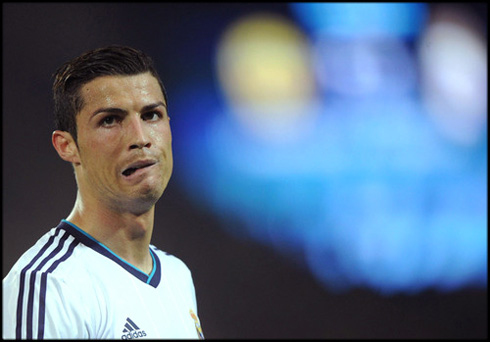
\includegraphics[width=\textwidth,height=0.8\textheight,keepaspectratio]
					{cr.jpg}
        }
        \only<5>{
\setbeamercolor{block title}{bg=red!50,fg=black}	
\setbeamercolor{block body}{bg=red!20,fg=black}
		\begin{block}{Ownership cycle}
			None of the 3 nodes ever gets deleted.
		\end{block}
        }

		\only<6>{
\setbeamercolor{block title}{bg=blue!15,fg=blue}	
\setbeamercolor{block body}{bg=blue!5,fg=black}
		\begin{block}{\texttt{weak\_ptr} edges}
			\texttt{weak\_ptr} holds a shared pointer but does not hold shared ownership.
			Allows to break the ownership dependency and avoid leaks.
		\end{block}}
		\begin{block}{Raw pointer edges}<7>
			No leaks are guaranteed by default by using only \texttt{unique\_ptr}
		\end{block}
	\end{columns}

	\begin{onlyenv}<3-4>
    \hrulefill
	\begin{lstlisting}
	==17575== 120 (40 direct, 80 indirect) bytes in 1 blocks are definitely lost 
	in loss record 3 of 3
	\end{lstlisting}
	\end{onlyenv}
	
	%\begin{onlyenv}<5->
	%\begin{lstlisting}
	%==1476== All heap blocks were freed -- no leaks are possible
	%\end{lstlisting}
	%\end{onlyenv}
	
\end{frame}

\begin{frame}[fragile,t]
\frametitle{Polymorphic types}
\framesubtitle{\texttt{unique\_ptr<T>}}

\tikzstyle{abstract}=[rectangle, draw=black, rounded corners, fill=blue!40, drop shadow,
        text centered, anchor=north, text=white, text width=3cm]
\tikzstyle{comment}=[rectangle, draw=black, rounded corners, fill=green, drop shadow,
        text centered, anchor=north, text=white, text width=3cm]
\tikzstyle{myarrow}=[->, >=open triangle 90, thick]
\tikzstyle{line}=[-, thick]
\setbeamertemplate{itemize/enumerate body begin}{\tiny}
	\begin{columns}[t]
	\column{0.5\textwidth}
		%\setbeamercovered{transparent}
		\begin{itemize}
			\item<2-> \texttt{Base} and \texttt{Derived} are related types.
			\item<3-> \texttt{Derived*} is convertible to \texttt{Base*}.
		\end{itemize}
		
		\begin{block}<3->{}
			\begin{lstlisting}
				Base* b = new Derived(); // OK
			\end{lstlisting}
		\end{block}
		\begin{itemize}
			\item<4-> \texttt{unique\_ptr<Base>} and \texttt{unique\_ptr<Derived>} are 
					  \textbf{NOT} related types
			\item<5-> Is \texttt{unique\_ptr<Derived>} convertible to \texttt{unique\_ptr<Base>}?
		\end{itemize}
		\begin{block}<5->{}
			\begin{lstlisting}
				std::unique_ptr<Base> b = 
					std::make_unique<Derived>() // OK???;
			\end{lstlisting}
		\end{block}
	\column{0.5\textwidth}
		\begin{tikzpicture}[baseline]<1->
			\node (Base) [abstract, rectangle split, rectangle split parts=2]
	        {
	            \textbf{Base}
	            %\nodepart{second}name
	        };
	   	 	\node (Derived) [abstract, rectangle split, rectangle split parts=2, below=of 
	   	 		   Base]
	        {
	            \textbf{Derived}
	            %\nodepart{second}nil
	        };
	        \draw[myarrow] (Derived.north) -- ++(0,0.8) -| (Base.south);
		\end{tikzpicture}
%		\newline
%		\begin{itemize}
%			\item<2> Base* and Derived* are related types.
%		\end{itemize}
	\end{columns}
\end{frame}

\begin{frame}[fragile]
\frametitle{\texttt{unique\_ptr} (less) simplified implementation}
\framesubtitle{Conversion construction \& assignment}
	\begin{columns}[t]
	\column{0.5\textwidth}
	\setbeamercovered{transparent}
		\begin{lstlisting}
			template <typename T>
			class unique_ptr
			{
			    T* _ptr = nullptr;
			public:
				/*..*/
				
				template <typename U>
				unique_ptr(unique_ptr<U>&& u)
				{
					static_assert(is_covertible<U*,T*>::value,
						"U not convertible to T");
					_ptr = u.release();
				}
				
				template <typename U>
				unique_ptr&
			    operator=(unique_ptr<U>&& u)
			    {
			    	static_assert(is_covertible<U*,T*>::value,
						"U not convertible to T");
			        reset(u.release());
			        return *this;
			    }		
			
				/*..*/
			};
		\end{lstlisting}
	\column{0.5\textwidth}
		\begin{block}{Constructor \& assigment operator}
			Take rvalue reference to a \texttt{unique\_ptr} which stores a different type
		\end{block}			
	\end{columns}
\end{frame}

\begin{frame}
	If \texttt{U*} is convertible to \texttt{T*} then
	\texttt{unique\_ptr<U>} is convertible to \texttt{unique\_ptr<T>}
\end{frame}

\begin{frame}[fragile,t]
\frametitle{Polymorphic types}
\framesubtitle{\texttt{unique\_ptr<T>}}
	\begin{lstlisting}
		struct Base
		{
			`virtual ~Base() = default;`
		};
	\end{lstlisting}
	\begin{lstlisting}	
		struct Derived : Base
		{
		};	
	\end{lstlisting}
    \hrulefill
	\begin{lstlisting}	
		std::unique_ptr<Base> b = std::make_unique<Derived>();
	\end{lstlisting}
    \hrulefill \newline
	Will work correctly \textbf{only} if the \texttt{Base} has virtual destructor.
	\pause
	\begin{block}{}
		\begin{lstlisting}
		template<class T,
				 class Deleter = std::default_delete<T>
		> class unique_ptr;
		\end{lstlisting}
	\end{block}
	The deleter is bound to type T. If destructor is not virtual then only Base class
	destructor will be called!
\end{frame}

\begin{frame}[fragile,t]
\setbeamerfont{normal text}{size=\tiny}
\frametitle{Non-virtual destructor case}
	\begin{lstlisting}
		struct Base
		{
			~Base() = default;
		};
	\end{lstlisting}
	\begin{lstlisting}	
		struct Derived : Base
		{
		};	

		template <typename T>
		struct MyDeleter
		{
		    template <typename U>
		    void operator()(U* p) const
		    {
		        delete static_cast<T*>(p);
		    }
		};
	\end{lstlisting}
			
    \hrulefill
	\begin{lstlisting}	
		std::unique_ptr<Base, MyDeleter<Derived>> b = std::make_unique<Derived>();
	\end{lstlisting}
    \hrulefill \newline
	The deleter is still bound to type T but the \texttt{operator()} will downcast
	the Base class to Derived insuring the Derived destructor to be called.
\end{frame}

\begin{frame}
    \begin{center}
		Assign a pointer of the Derived class to a pointer to the Base class 
		only when the Base class has virtual destructor.
    \end{center}
\end{frame}

\begin{frame}[fragile,t]
\frametitle{More on polymorphic types}
\framesubtitle{\texttt{unique\_ptr<T>}}

\tikzstyle{abstract}=[rectangle, draw=black, rounded corners, fill=blue!40, drop shadow,
        text centered, anchor=north, text=white, text width=3cm]
\tikzstyle{comment}=[rectangle, draw=black, rounded corners, fill=green, drop shadow,
        text centered, anchor=north, text=white, text width=3cm]
\tikzstyle{myarrow}=[->, >=open triangle 90, thick]
\tikzstyle{line}=[-, thick]
\setbeamertemplate{itemize/enumerate body begin}{\tiny}

	\begin{columns}[t]
	\column{0.5\textwidth}
		%\setbeamercovered{transparent}
		\begin{itemize}
			\item<1-> \texttt{Base} and \texttt{Derived} are related types.
			\item<1-> \texttt{Derived*} is converitble to \texttt{Base*}.
			\item<2-> \texttt{Base*} can be casted to \texttt{Derived*}
		\end{itemize}
		
		\begin{block}<2->{}
			\begin{lstlisting}
				Base* b = new Derived(); // OK
				auto* d = static_cast<Derived*>(b); // OK
			\end{lstlisting}
		\end{block}
			
		\begin{itemize}
			\item<1-> \texttt{unique\_ptr<Base>} and \texttt{unique\_ptr<Derived>} are 
					  \textbf{NOT} related types
			\item<1-> \texttt{unique\_ptr<Derived>} is convertible to 
					  \texttt{unique\_ptr<Base>}
			\item<3-> \texttt{unique\_ptr<Base>} \textbf{CANNOT} be casted to 
					  \texttt{unique\_ptr<Derived>}
		\end{itemize}
		\begin{block}<3->{}
			\begin{lstlisting}
				std::unique_ptr<Base> b = 
					std::make_unique<Derived>() // OK;
				auto d = static_cast<
						std::unique_ptr<Derived>>(b); // error
			\end{lstlisting}
		\end{block}
	\column{0.5\textwidth}
		\begin{tikzpicture}[baseline]<1->
			\node (Base) [abstract, rectangle split, rectangle split parts=2]
	        {
	            \textbf{Base}
	            %\nodepart{second}name
	        };
	   	 	\node (Derived) [abstract, rectangle split, rectangle split parts=2, below=of 
	   	 		   Base]
	        {
	            \textbf{Derived}
	            %\nodepart{second}nil
	        };
	        \draw[myarrow] (Derived.north) -- ++(0,0.8) -| (Base.south);
		\end{tikzpicture}
	\end{columns}
\end{frame}

\begin{frame}[fragile]
	\onslide<1->
	A \texttt{unique\_ptr<U>} can only be moved to \texttt{unique\_ptr<T>} if U* is convertible to T*.
	\begin{example}
		\begin{lstlisting}
			auto d = std::make_unique<Derived>();
			std::unique_ptr<Base> b = std::move(d);
			auto d_ptr = static_cast<Derived*>(b.get());
		\end{lstlisting}
	\end{example}
\setbeamercolor{block title example}{bg=red!50,fg=black}	
\setbeamercolor{block body example}{bg=red!20,fg=black}
	\onslide<2->
	There is no cast semantics for \texttt{unique\_ptr}!
	\begin{example}
		\begin{lstlisting}
			std::unique_ptr<Base> b = std::make_unique<Derived>();
			auto d = static_cast<Derived>(b); // error
		\end{lstlisting}
	\end{example}
\end{frame}

\begin{frame}
    \begin{center}
        (The less casting in the code the better)
    \end{center}
\end{frame}

\begin{frame}[fragile,t]
\frametitle{Polymorphic types}
\framesubtitle{\texttt{shared\_ptr<T>}}

\tikzstyle{abstract}=[rectangle, draw=black, rounded corners, fill=blue!40, drop shadow,
        text centered, anchor=north, text=white, text width=3cm]
\tikzstyle{comment}=[rectangle, draw=black, rounded corners, fill=green, drop shadow,
        text centered, anchor=north, text=white, text width=3cm]
\tikzstyle{myarrow}=[->, >=open triangle 90, thick]
\tikzstyle{line}=[-, thick]
\setbeamertemplate{itemize/enumerate body begin}{\tiny}

	\begin{columns}[t]
	\column{0.5\textwidth}
		%\setbeamercovered{transparent}
		\begin{itemize}
			\item<1-> \texttt{shared\_ptr<Base>} and \texttt{shared\_ptr<Derived>} are 
					  \textbf{NOT} related types
			\item<2-> \texttt{shared\_ptr<Derived>} is convertible to 
					  \texttt{shared\_ptr<Base>}
			\item<3-> \texttt{shared\_ptr<Base>} \textbf{CAN} be casted to 
					  \texttt{shared\_ptr<Derived>}
		\end{itemize}
		\begin{block}<3->{}
			\begin{lstlisting}
				std::shared_ptr<Base> b = 
					std::make_shared<Derived>() // OK;
				auto d = std::static_pointer_cast<
						std::shared_ptr<Derived>>(b); // OK
			\end{lstlisting}
		\end{block}
	\column{0.5\textwidth}
		\begin{tikzpicture}[baseline]<1->
			\node (Base) [abstract, rectangle split, rectangle split parts=2]
	        {
	            \textbf{Base}
	            %\nodepart{second}name
	        };
	   	 	\node (Derived) [abstract, rectangle split, rectangle split parts=2, below=of 
	   	 		   Base]
	        {
	            \textbf{Derived}
	            %\nodepart{second}nil
	        };
	        \draw[myarrow] (Derived.north) -- ++(0,0.8) -| (Base.south);
		\end{tikzpicture}
	\end{columns}
\end{frame}

\begin{frame}[fragile]
	\onslide<1->
	A \texttt{shared\_ptr<U>} defines casting semantics for all 4 cast types:
	\begin{itemize}
		\item \texttt{static\_pointer\_cast}
		\item \texttt{dynamic\_pointer\_cast}
		\item \texttt{const\_pointer\_cast}
		\item \texttt{reinterpret\_pointer\_cast}
	\end{itemize}
	\begin{example}
		\begin{lstlisting}
			std::shared_ptr<Base> b = std::make_shared<Derived>()
			auto d = std::static_pointer_cast<std::shared_ptr<Derived>>(b);
		\end{lstlisting}
	\end{example}
\setbeamercolor{block title example}{bg=red!50,fg=black}	
\setbeamercolor{block body example}{bg=red!20,fg=black}
	\onslide<2->
	but ... \newline
	... this is expensive
\end{frame}

\begin{frame}[fragile,t]
	Remember: \texttt{shared\_ptr<Base>} and \texttt{shared\_ptr<Derived>} are 
					  \textbf{unrelated} types \newline \newline
	
	\begin{lstlisting}
		template< class T, class U > 
		std::shared_ptr<T> static_pointer_cast(const std::shared_ptr<U>& r)
		{
		    auto p = static_cast<T*>(r.get());
		    return std::shared_ptr<T>(r, p);
		}
	\end{lstlisting}
	\pause
	 Here casting actually means creating another \texttt{shared\_ptr} instance.
	\pause
	\begin{block}{Aliasing constructor}
		An \textit{aliasing constructor} - \texttt{shared\_ptr} shares
			  ownership with \texttt{r} but stores \texttt{p}
	\end{block}
\end{frame}

\begin{frame}
    \begin{center}
        What about \texttt{raw pointers}?
    \end{center}
\end{frame}

\begin{frame}[fragile]
\frametitle{Raw pointers are still OK}
	Function parameters where the function performs read or write operations
	on the object but \textbf{does not become the owner}
	\begin{example}
		\begin{lstlisting}
			void func(MyClass* obj);
			void func(const MyClass* obj);
		\end{lstlisting}
	\end{example}
\end{frame}

\begin{frame}[fragile]
\frametitle{Raw pointers are still OK}
	Return types from a function where the caller \textbf{does not become the owner}
	\begin{example}
		\begin{lstlisting}
			std::map<int, std::unique_ptr<MyClass>> cache;
			
			MyClass* makeAndSaveObj(int index)
			{
				auto obj = std::make_unique<MyClass>();
				auto ptr = obj.get();
				// Do something with obj
				cache.insert({index, std::move(obj)});
				return ptr;
			}
		\end{lstlisting}
	\end{example}
\end{frame}

\begin{frame}[fragile,t]
\frametitle{Objects in containers}
    \begin{lstlisting}
        struct Foo
        {
            int i;
            double d;
            char ch[10];
            long long long_int;
        };
    \end{lstlisting}

    \only<2>{
    \begin{center}
    Store Foo in a container as value or pointer?
    \newline
    \newline
    \texttt{std::vector<Foo>}
    \newline
    or
    \newline
    \texttt{std::vector<std::unique\_ptr<Foo>>}
    \end{center}
    }

    \only<3>{
    \begin{table}
    \begin{tabular}{l | c | c | c}
        Operation & \texttt{vector<Foo>} & \texttt{vector<unique\_ptr<Foo>>} \\
        \hline \hline
        push\_back & 0.0324s & 0.0382s  \\
        push\_back (\textit{reserve}) & 0.0093s & 0.0331s  \\
        traverse & 0.0021s & 0.0032s \\ 
        sort & 0.2009s & 0.2167s
    \end{tabular}
    \caption{1M elements}
    \end{table}
    }
\end{frame}

\begin{frame}[fragile,t]
    \newcommand{\element}[2]{
		\foreach \r in {#1} {%
  			\globaldefs=1\relax
  			\tikzset{row \r/.style={nodes={fill=#2}}}
		}%
	}
    \begin{columns}[T]
	\column{0.5\textwidth}
        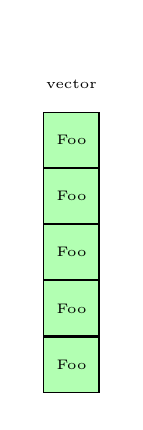
\begin{tikzpicture}[font=\ttfamily,
            vector/.style={matrix of nodes,nodes={draw, minimum size=7mm, fill=green!30},
            column sep=-\pgflinewidth, row sep=0.0mm, nodes in empty cells, font=\tiny,
            row 1/.style={nodes={draw=none, fill=none}}}]
            
            \matrix[vector, label={}] (vec) {
            vector \\Foo \\Foo \\Foo \\Foo \\Foo \\};
        \end{tikzpicture}
        \begin{block}{}
            Traversing data in contiguous memory.
        \end{block}
    \column{0.5\textwidth}
        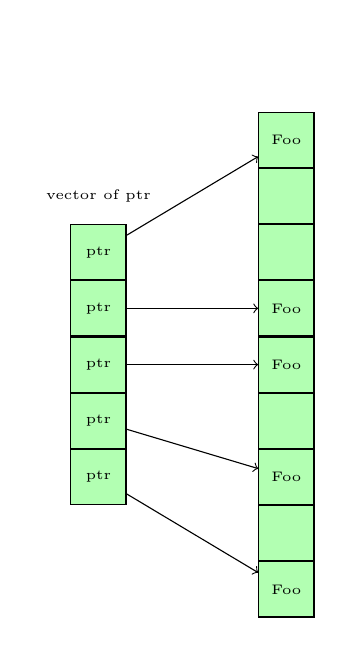
\begin{tikzpicture}[font=\ttfamily,
            vector/.style={matrix of nodes,nodes={draw, minimum size=7mm, fill=green!30},
            column sep=-\pgflinewidth, row sep=0.0mm, nodes in empty cells, font=\tiny,
            row 1/.style={nodes={draw=none, fill=none}}}]
            
            \matrix[vector, label={}] (vec) {
                vector of ptr \\ptr \\ptr \\ptr \\ptr \\ptr \\};
            \element{3,4,7,9}{red!30}
            \matrix[vector, right=of vec, label={}] (mem) {
                \\Foo \\ \\ \\Foo \\Foo \\ \\Foo \\ \\Foo \\};
			\draw[->](vec-2-1) -- (mem-2-1);
			\draw[->](vec-3-1) -- (mem-5-1);
			\draw[->](vec-4-1) -- (mem-6-1);
			\draw[->](vec-5-1) -- (mem-8-1);
			\draw[->](vec-6-1) -- (mem-10-1);
            %\draw (v2-1-6.south)--++(45:-5mm) node [below] {median};
        \end{tikzpicture}
        \begin{block}{}
            Traversing data in sparse memory.
        \end{block}
    \end{columns}
\end{frame}

\begin{frame}[fragile,t]
\frametitle{Objects in containers}
    \begin{lstlisting}
        struct BigFoo
        {
            int i;
            double d;
            char ch[1000];
            long long long_int;
        };
    \end{lstlisting}

    \only<2>{
    \begin{table}
    \begin{tabular}{l | c | c | c}
        Operation & \texttt{vector<BigFoo>} & \texttt{vector<unique\_ptr<BigFoo>>} \\
        \hline \hline
        push\_back & 0.7142 & 0.3237s  \\
        push\_back (\textit{reserve}) & 0.150 & 0.262s  \\
        traverse & 0.0088s & 0.0095s \\ 
        sort & 1.415s & 0.2605s
    \end{tabular}
    \caption{1M elements}
    \end{table}
    }
\end{frame}

\begin{frame}
    Store non-polymorphic objects as pointers in STL containers if:
    \begin{itemize}
        \item Their size is big
        \item Mutating algorithms will be run on the container.
    \end{itemize}
    In other case prefer storing object as values.
\end{frame}

\begin{frame}[fragile,t]
\frametitle {Moving objects}
\setbeamercovered{transparent}
    \begin{lstlisting}
        |\onslide<1->|
        struct Buffer
        {   |\onslide<1>|
            Buffer(size_t s) : data{new int[s]}, size{s} {} |\onslide<2>|
            Buffer(const BigObject& other)
            {
                data.reset(new int[other.size]);
                size = other.size;
                std::copy(other.data.get(), other.data.get() + other.size, data.get());
            } |\onslide<3>|
            Buffer(BigObject&& other)
            {
                data.swap(other.data);
                size = other.size;
            }
            |\onslide<1-3>|
            std::unique_ptr<int[]> data;
            size_t size; |\onslide<1->|
        };
    \end{lstlisting}
    \begin{onlyenv}<4>
    \begin{lstlisting}
        std::vector<Buffer> vec;
        vec.reserve(10);
        for (auto i = 1; i <= 15; i++)
        {
            vec.push_back(Buffer{100000000});
        }
    \end{lstlisting}
    \end{onlyenv}
\end{frame}

\begin{frame}
	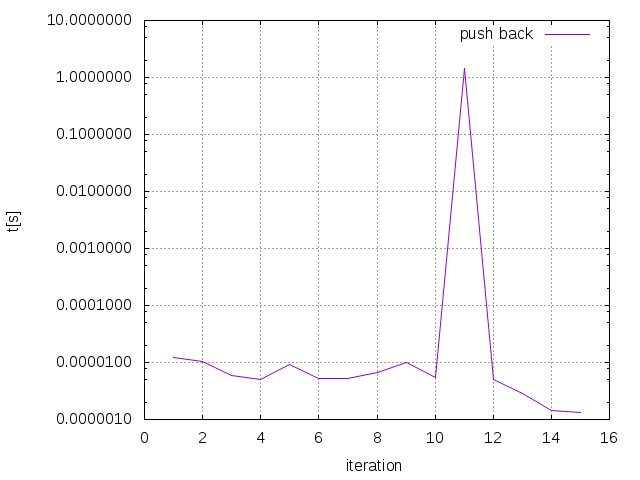
\includegraphics[width=\textwidth,height=0.8\textheight,keepaspectratio]
					{move_without_noexcept.jpeg}
\end{frame}

\begin{frame}[fragile]
    \begin{onlyenv}<1>
    \begin{lstlisting}
        struct Buffer
        {
            Buffer(size_t s) : data{new int[s]}, size{s} {}
            `Buffer(const Buffer& other)`
            {
                data.reset(new int[other.size]);
                size = other.size;
                std::copy(other.data.get(), other.data.get() + other.size, data.get());
            }
            `Buffer(Buffer&& other)`
            {
                data.swap(other.data);
                size = other.size;
            }

            std::unique_ptr<int[]> data;
            size_t size;
        };
    \end{lstlisting}
    \end{onlyenv}
    \begin{onlyenv}<2>
    \begin{lstlisting}
        struct Buffer
        {
            Buffer(size_t s) : data{new int[s]}, size{s} {}
            `Buffer(const Buffer& other)`
            {
                data.reset(new int[other.size]);
                size = other.size;
                std::copy(other.data.get(), other.data.get() + other.size, data.get());
            }
            `Buffer(Buffer&& other) noexcept`
            {
                data.swap(other.data);
                size = other.size;
            }

            std::unique_ptr<int[]> data;
            size_t size;
        };
    \end{lstlisting}
    \end{onlyenv}
    \begin{alertblock}{Strong exception guarantee}<1>
        During re-allocation \texttt{std::vector} uses \texttt{move\_if\_no\_except} function to move
        elements from the old to the new buffer.
        If the move constructor has no noexcept qualifier it will resort to copy.
    \end{alertblock}
\end{frame}

\begin{frame}
	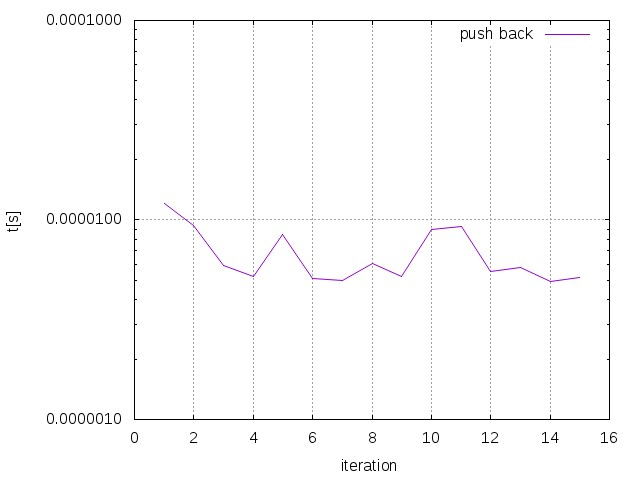
\includegraphics[width=\textwidth,height=0.8\textheight,keepaspectratio]
					{move_with_noexcept.jpeg}
\end{frame}

\begin{frame}[fragile,t]
\frametitle{\texttt{move\_if\_noexcept}}
    \begin{onlyenv}<1-2>
    \begin{block}{move\_if\_noexcept}
    \begin{lstlisting}
    template <class T>
    typename std::conditional<!std::is_nothrow_move_constructible<T>::value &&
                                  std::is_copy_constructible<T>::value,
                              const T&,
                              T&&>::type
    move_if_noexcept(T& x) noexcept
    {
        using type =
            typename std::conditional<!std::is_nothrow_move_constructible<T>::value &&
                                          std::is_copy_constructible<T>::value,
                                      const T&, T &&>::type;

        return static_cast<type>(x);
    }
    \end{lstlisting}
    \end{block}
    \end{onlyenv}

    \begin{onlyenv}<3>
    \begin{block}{move\_if\_noexcept}
    \begin{lstlisting}
    template <class T>
    typename std::conditional<!std::is_nothrow_move_constructible<T>::value &&
                                  std::is_copy_constructible<T>::value,
                              const T&,
                              T&&>::type
    move_if_noexcept(T& x) noexcept;
    \end{lstlisting}
    \end{block}
    \end{onlyenv}
    
    \begin{onlyenv}<2>
    \begin{block}{conditional}
    \begin{lstlisting}
    template<bool B, typename T, typename U>
    struct conditional { using type  = T; };
    
    template<typename T, typename U>
    struct conditional<false, T, U> { using type = U; };
    \end{lstlisting}
    \end{block}
    \end{onlyenv}

    \begin{onlyenv}<3>
    \begin{lstlisting}
    struct A
    {
        A() = default;
        A(const A&) {/**/}
        A(A&&) {/**/}
    };
    struct B
    {
        B() = default;
        B(const B&) {/**/}
        B(B&&) noexcept {/**/}
    };
    \end{lstlisting}
    \hrulefill
    \begin{lstlisting}
    A a;
    B b;
    auto a2 = std::move_if_noexcept(a); // copy
    auto b2 = std::move_if_noexcept(b); // move
    \end{lstlisting}
    \end{onlyenv}
\end{frame}

\begin{frame}
    \begin{center}
    Prefer storing non-polymorphic objects as values in STL containers. \newline \newline
    If \texttt{move} operation is expensive reserve the memory first (\texttt{vector}). \newline \newline
    \pause
    Make sure the move constructor is \texttt{noexcept}.
    \end{center}
\end{frame}

\begin{frame}
\frametitle{Resource Acquisition Is Initialization (RAII)}
    \pause
    \begin{center}
        One the the most fundamental techniques in C++.
        \newline
        Facilitates automatic resource cleanup to prevent leaks.
    \end{center}
\end{frame}
\begin{frame}
\frametitle{Resource Acquisition Is Initialization (RAII)}
    \begin{itemize}
        \item memory
        \item files
        \item directories
        \item file descriptors
        \item mutexes,locks
    \end{itemize}
\end{frame}


\begin{frame}[fragile]
\frametitle{Resource Acquisition Is Initialization (RAII)}
    \pause
    \begin{block}{Memory}
        \begin{lstlisting}
            {
                std::unique_ptr<Foo> f{new Foo{}};
            }
            // f is deleted, memory is free
        \end{lstlisting}
    \end{block}
    
    \pause
    \begin{block}{File handle}
        \begin{lstlisting}
            {
                std::ofstream f("file.txt");
            }
            // file handle resource is encapsulated in the ofstream class
        \end{lstlisting}
    \end{block}

    \pause
    \begin{block}{Mutex}
        \begin{lstlisting}
            std::mutex gmutex;
            {
                std::lock_guard<std::mutex> lock{gmutex};   
            }
            // mutex is unlocked
        \end{lstlisting}
    \end{block}
\end{frame}

\begin{frame}[fragile,t]
\frametitle{Resource Acquisition Is Initialization (RAII)}
\framesubtitle{Directory handle}
    \begin{onlyenv}<1-2>
    \begin{lstlisting}
        {
            std::filesystem::path p{"dirname"};
            for (auto& x : std::filesystem::directory_iterator(p))
            {
                // ...
            }
            // file handle resource is encapsulated in the directory_entry class
        }
    \end{lstlisting}
    \end{onlyenv}

    \begin{onlyenv}<3>
    \begin{lstlisting}
        {
            boost::filesystem::path p{"dirname"};
            for (auto& x : boost::filesystem::directory_iterator(p))
            {
                // ...
            }
            // file handle resource is encapsulated in the directory_entry class
        }
    \end{lstlisting}
    \end{onlyenv}

    \begin{onlyenv}<4>
    \begin{lstlisting}
        {
            DIR* dir = opendir("dirname");
            if (dir)
            {
                struct dirent* dent;
                while(dent=readdir(dir))
                {
                    //...
                }
            }
            close(dir);
        }
    \end{lstlisting}
    \end{onlyenv}

    \begin{onlyenv}<2>
    \begin{block}{New STL feature}
        Standard \texttt{filesystem} library is only available since C++17.
    \end{block}
    \end{onlyenv}

    \begin{onlyenv}<3>
    \begin{block}{Also available in boost}
        When using compiler not supporting C++17, the \texttt{filesystem} library is available in boost.
    \end{block}
    \end{onlyenv}

    \begin{onlyenv}<4>
    \begin{alertblock}{C API}
        Prefer using the \texttt{std} or \texttt{boost} \texttt{filesystem} library over the C API. 
    \end{alertblock}
    \end{onlyenv}
\end{frame}

\begin{frame}
\frametitle{Resource Acquisition Is Initialization (RAII)}
    \begin{center}
        If a standard library (or boost) does not provide RAII wrapper for a given resource, write your own.       
    \end{center}
\end{frame}

\begin{frame}[fragile,t]
\frametitle{Resource Acquisition Is Initialization (RAII)}
\framesubtitle{File descriptor}
    \begin{lstlisting}
        {
            int fd = socket(/*...*/)
            if (fd != -1)
            {
                //...
            }

            close(fd);
        }
        {
            int fd = open("/dev/random");
            if (fd != -1)
            {
                //...
            }

            close(fd);
        }
    \end{lstlisting}
\end{frame}

\begin{frame}[fragile,t]
\frametitle{Resource Acquisition Is Initialization (RAII)}
\framesubtitle{File descriptor}
    \begin{onlyenv}<1>
    \begin{lstlisting}
        class FileDescriptor
        {
            int mFd = -1;
        public:
            FileDescriptor(int fd) : mFd{fd}
            {
                if (mFd < 0)
                {
                    throw std::invalid_argument { "Invalid descriptor." };
                }
            }

            ~FileDescriptor()
            {
                if ( -1 == ::close(mFd) )
                {
                    // perhaps log some error
                }  
            }

            int get() const { return mFd; }

            operator int() const { return get(); }
        };
    \end{lstlisting}
    \end{onlyenv}
    
    \begin{onlyenv}<2>
    \begin{lstlisting}
        class FileDescriptor
        {
            int mFd = -1;
        public:
            /*
             ...
            */

            FileDescriptor(const FileDescriptor&) = delete;
            FileDescriptor& operator=(const FileDescriptor&) = delete;

            FileDescriptor(FileDescriptor&& other) noexcept
            {
                mFd = other.mFd;
                other.mFd = -1;
            }
            FileDescriptor& operator=(FileDescriptor&& other) noexcept
            {
                mFd = other.mFd;
                other.mFd = -1;
                return *this;
            }
        };
    \end{lstlisting}
    \end{onlyenv}
\end{frame}

\begin{frame}[fragile,t]
\frametitle{Resource Acquisition Is Initialization (RAII)}
\framesubtitle{File descriptor}
    \begin{onlyenv}<1>
    \begin{lstlisting}
        {
            int fd = socket(/*...*/)
            if (fd != -1)
            {
                //...
            }

            close(fd);
        }
        {
            int fd = open("/dev/random");
            if (fd != -1)
            {
                //...
            }

            close(fd);
        }
    \end{lstlisting}
    \end{onlyenv}
    
    \begin{onlyenv}<2>
    \begin{lstlisting}
        {
            try 
            {
                FileDescriptor fd{socket(/*...*/)};
            }
            catch(const std::invalid_argument& e) {}
        }
        {
            try 
            {
                FileDescriptor fd{open("/dev/random")};
            }
            catch(const std::invalid_argument& e) {}
        }
    \end{lstlisting}
    \end{onlyenv}
\end{frame}

\section{Function parameters}

\begin{frame}
    \begin{center}
        Function parameters.
    \end{center}
\end{frame}

\begin{frame}
\frametitle{Motivation}
    \begin{itemize}
        \item C++ offers a variaty of options to pass parameters to functions
        \pause
        \item With C++11 came r-value references and smart pointers adding more options
        \pause
        \item In many cases more than 1 option will work but usually only 1 makes the most sense
    \end{itemize}
\end{frame}

\begin{frame}
\setbeamertemplate{itemize/enumerate body begin}{\tiny}
    \begin{itemize}
			\item \texttt{fun(int p)}
			\item \texttt{fun(MyClass* p)}
			\item \texttt{fun(const MyClass* p)}
			\item \texttt{fun(MyClass\& p)}
			\item \texttt{fun(const MyClass\& p)}
			\item \texttt{fun(MyClass** p)}
			\item \texttt{fun(MyClass*\& p)}
			\item \texttt{fun(MyClass*** p)}
			\item ...
            \pause \newline
			\item \texttt{fun(MyClass\&\& p)}
			\item \texttt{fun(unique\_ptr<MyClass> p)}
			\item \texttt{fun(shared\_ptr<MyClass> p)}
			\item \texttt{fun(const shared\_ptr<MyClass>\& p)}
			\item \texttt{template<class T> fun(T\&\& p)}
			\item ...
    \end{itemize}
\end{frame}

\begin{frame}[fragile,t]
\frametitle{Sinking value}
\framesubtitle{C++03 approach}
\setbeamercovered{transparent}
	\begin{lstlisting}
        class MyClass
        {|\onslide<1>|
            std::string mName;|\onslide<2>|
            int mCount = 0;|\onslide<1->|
        public:|\onslide<1>|
            void setName(const std::string& name)
            {
                mName = name;
            }|\onslide<2>|
            
            void setCount(int count) 
            {
                mCount = count;
            }|\onslide<1->|
        };	
	\end{lstlisting}
	
\setbeamercovered{invisible}
    \only<1>{
    \begin{block}{Pass by reference}
        Copying object is expensive.
    \end{block}}

    \only<2>{
    \begin{block}{Pass by value}
        Copying object is cheap.
    \end{block}}

\end{frame}

\begin{frame}
\frametitle{Sinking value}
    \begin{center}
        With C++11 standard the common way of sinking value has changed.
    \end{center}
\end{frame}

\begin{frame}[fragile,t]
\frametitle{Sinking value}
	\begin{columns}[T]
	\column{0.5\textwidth}
        \begin{lstlisting}
            class MyClass
            {
                std::string mName;
            public:		
                void setName(std::string name) 
                {
                    mName = std::move(name);
                }
            };	
        \end{lstlisting}
        \hrulefill
        \begin{lstlisting}
            MyClass m;
            std::string s1 = "Yoda";
            m.setName(s1); // copy + move
            m.setName("Luke"); // move
            m.setName(std::move(s1)); // move + move
        \end{lstlisting}
	\column{0.5\textwidth}
        \begin{onlyenv}<3>
        \begin{lstlisting}
            class MyClass
            {
                std::string mName;
            public:		
                void setName(const std::string& name) 
                {
                    mName = name;
                }
            };	
        \end{lstlisting}
        \hrulefill
        \begin{lstlisting}
            MyClass m;
            std::string s1 = "Yoda";
            m.setName(s1); // copy
            m.setName("Luke"); // copy
            m.setName(std::move(s1)); // copy
        \end{lstlisting}
        \end{onlyenv}
	\end{columns}

    \only<2>{
    \begin{block}{Pass by value}
        Moving object is cheap.
    \end{block}}
\end{frame}

\begin{frame}[fragile,t]
\frametitle{Sinking value}
\setbeamercovered{transparent}
	\begin{lstlisting}
        struct Data
        {
            Data() = default;|\onslide<2->|
            Data(const Data& d)
            {
                std::copy_n(d.buff, 1000, buff);
            }
            |\onslide<3->|
            Data(Data&& d)
            {
                std::copy_n(d.buff, 1000, buff);
            }
            |\onslide<1->|
            char buff[1000];
        };
	\end{lstlisting}

\setbeamercovered{invisible}

	\begin{columns}[T]
	\column{0.5\textwidth}
        \begin{onlyenv}<4-6>
        \begin{lstlisting}
            class MyClass
            {
                Data mData;
            public:		
                void setData(Data data)
                {
                    mData = std::move(data);
                }
            };
        \end{lstlisting}
        \end{onlyenv}
        \begin{onlyenv}<7->
        \begin{lstlisting}
            class MyClass
            {
                Data mData;
            public:		
                void setData(Data&& data)
                {
                    mData = std::move(data);
                }
            };
        \end{lstlisting}
        \end{onlyenv}
	\column{0.5\textwidth}
        \only<6>{
        \begin{alertblock}{Not efficient}
            The object is moved twice.
        \end{alertblock}}
        \only<8>{
        \begin{block}{Efficient}
            The object is moved only once.
        \end{block}}
    \end{columns}
    \hrulefill
    \begin{onlyenv}<5-6>
    \begin{lstlisting}
        MyClass m;
        Data d;
        m.setData(std::move(d)); // move + move
    \end{lstlisting}
    \end{onlyenv}
    \begin{onlyenv}<7->
    \begin{lstlisting}
        MyClass m;
        Data d;
        m.setData(std::move(d)); // move
    \end{lstlisting}
    \end{onlyenv}
\end{frame}

\begin{frame}[fragile,t]
\frametitle{Sinking value}
    \begin{onlyenv}<1-2>
    \begin{lstlisting}
        class MyClass
        {
            Data mData;
        public:		
            void setData(Data&& data)
            {
                mData = std::move(data);
            }
        };
    \end{lstlisting}
    \end{onlyenv}

    \begin{onlyenv}<3->
    \begin{lstlisting}
        class MyClass
        {
            Data mData;
        public:		
            void setData(Data&& data)
            {
                mData = std::move(data);
            }
            void setData(const Data& data)
            {
                mData = data;
            }
        };
    \end{lstlisting}
    \end{onlyenv}

    \hrulefill
    \begin{onlyenv}<1>
    \begin{lstlisting}
        MyClass m;
        Data d;
        m.setData(d);
    \end{lstlisting}
    \end{onlyenv}

    \begin{onlyenv}<2->
    \begin{lstlisting}
        MyClass m;
        Data d;
        `m.setData(d);`
    \end{lstlisting}
    \end{onlyenv}

    \begin{onlyenv}<2>
    \begin{alertblock}{Compiler error}
        Passing l-value reference to a function which takes r-value reference.       
    \end{alertblock}
    \end{onlyenv}

    \begin{onlyenv}<3>
    \begin{block}{OK}
        Another overload which takes l-value reference.
    \end{block}
    \end{onlyenv}
\end{frame}

\begin{frame}[fragile]
\frametitle{Sinking value}
	Prefer passing by value when \texttt{move} operation for the passed object is cheap.
	\begin{example}
		\begin{lstlisting}
			class MyClass
			{
				std::string mName;
			public:
				MyClass(std::string name) : mName{std::move(name)}{}
				void setName(std::string name) {mName = std::move(name);}	
			};	
		\end{lstlisting}
	\end{example}
\end{frame}

\begin{frame}[fragile]
\frametitle{Sinking value}
	Prefer passing by r-value when \texttt{move} operation for the passed object is expensive.
	\begin{example}
		\begin{lstlisting}
			class MyClass
			{
				BigData mData;
			public:
				MyClass(const BigData& data) : mData{data}{}
				MyClass(BigData&& data) : mData{std::move(data)}{}
				void setData(const BigData& data) {mData = data;}	
				void setData(BigData&& data) {mData = std::move(data);}		
			};	
		\end{lstlisting}
	\end{example}
\end{frame}

\begin{frame}[fragile,t]
\frametitle{Ownership transfer}
	\begin{columns}[T]
	\column{0.5\textwidth}
        \begin{onlyenv}<1-2>
        \begin{lstlisting}
			void f(std::unique_ptr<A> a)
			{
			}	
		\end{lstlisting}
        \end{onlyenv}
        \begin{onlyenv}<3->
        \begin{lstlisting}
			void f(std::unique_ptr<A> a)
			{
            //ownership has already been transferred 
            //from caller

			}	
		\end{lstlisting}
        \end{onlyenv}
    
        \hrulefill
        \begin{onlyenv}<1-3>
        \begin{lstlisting}
            auto ptr = std::make_unique<A>();
            f(std::move(ptr));
		\end{lstlisting}
        \end{onlyenv}

        \begin{onlyenv}<4->
        \begin{lstlisting}
            auto ptr = std::make_unique<A>();
            f(std::move(ptr));
            // ptr has nullptr value
		\end{lstlisting}
        \end{onlyenv}

        \begin{block}{Guaranteed ownership transfer}<4->
            Passing \texttt{unique\_ptr} by value so the ptr is moved to function argument.
        \end{block}

        \column{0.5\textwidth}
        \begin{onlyenv}<1-2>
        \begin{lstlisting}
			void f(std::unique_ptr<A>&& a)
			{
			}	
		\end{lstlisting}
        \end{onlyenv}

        \begin{onlyenv}<3->
        \begin{lstlisting}
			void f(std::unique_ptr<A>&& a)
			{
            //ownership has not yet been transferred 
            //from caller. 
            //Only the reference has been passed.
			}	
		\end{lstlisting}
        \end{onlyenv}

        \hrulefill
        \begin{onlyenv}<1-3>
        \begin{lstlisting}
            auto ptr = std::make_unique<A>();
            f(std::move(ptr));
		\end{lstlisting}
        \end{onlyenv}

        \begin{onlyenv}<4->
        \begin{lstlisting}
            auto ptr = std::make_unique<A>();
            f(std::move(ptr));
            //ptr may or may not have nullptr value
		\end{lstlisting}
        \end{onlyenv}

        \begin{block}{Potential ownership transfer}<4->
            Passing \texttt{unique\_ptr} by reference so the ptr is \textbf{NOT} moved function argument.
            It may or may not be moved inside the function.
        \end{block}
	\end{columns}

    \only<2>{
        \begin{center}
            What's the difference?
        \end{center}
    }

    \only<5>{
        \begin{center}
            Calling \texttt{std::move} does not imply that anything is being moved.
        \end{center}
    }
\end{frame}

\begin{frame}[fragile,t]
\frametitle{\texttt{std::move}}
    \begin{block}{Standard implementation}
        \begin{lstlisting}
            /**
             *  @brief  Convert a value to an rvalue.
             *  @param  __t  A thing of arbitrary type.
             *  @return The parameter cast to an rvalue-reference to allow moving it.
             */
            template<typename _Tp>
            constexpr typename std::remove_reference<_Tp>::type&&
            move(_Tp&& __t) noexcept
            { return static_cast<typename std::remove_reference<_Tp>::type&&>(__t); }
        \end{lstlisting}
    \end{block}
    
    \pause
    \texttt{std::move} does not move anything. Just casts to r-value reference. \newline \newline
    \pause
    The actual moving happens in \texttt{move constructor} or \texttt{move assigment operator}.
\end{frame}

\begin{frame}
\frametitle{\texttt{shared\_ptr<T>}}
    \only<1>{
    \begin{center}
        Where could we use it?
    \end{center}}
    \only<2>{
    \begin{center}
        Event loop example...
    \end{center}}
\end{frame}

\begin{frame}[fragile]
\setbeamercovered{transparent}
	\begin{onlyenv}<1->
	\begin{lstlisting}
		|\onslide<3>|
		struct TransactionContext
		{
			...
			std::vector<Object> objectsCreated;
			std::vector<Object> objectsDeleted;
			std::vector<Message> messagesToSend;
			...
		};
	\end{lstlisting}
	\end{onlyenv}
	\begin{onlyenv}<1->
	\begin{lstlisting}
		|\onslide<2->|
		void processEvent(const Event& e, TransactionContext& context){...}
		void commitTransaction(const TransactionContext& context){...}
		void sendMessages(const TransactionContext& context){...}
	\end{lstlisting}
	\end{onlyenv}
	\begin{onlyenv}<1->
	\begin{lstlisting}
		|\onslide<1->|
		void evtLoop()
		{
			while (true)
			{ 
				auto event = receiveEvent();
				TransactionContext context;
				processEvent(event,  context);
				commitTransaction(context);
				sendMessages(context);
			}
		}
	\end{lstlisting}
	\end{onlyenv}
\end{frame}

\begin{frame}[fragile,t]
\setbeamercovered{transparent}
	\begin{onlyenv}<1-6>
	\begin{lstlisting}
		void sendMessages(const TransactionContext& context)
		{
			for (const auto& m : context.messagesToSend)
			{
				auto sent = send(m);
				if (!sent) {...}
			}
		}
	\end{lstlisting}
	\end{onlyenv}
	
	\begin{onlyenv}<7>
	\begin{lstlisting}
		void sendMessages(`std::shared_ptr<TransactionContext>` context)
		{
			for (const auto& m : context->messagesToSend)
			{
				auto sent = send(m); //synchronous send
				if (!sent) {...}
			}
		}
	\end{lstlisting}
	\end{onlyenv}

    %\begin{onlyenv}<8->
	%\begin{lstlisting}
%		void sendMessages(`std::shared_ptr<const TransactionContext>` context)
%		{
%			for (const auto& m : context->messagesToSend)
%			{
%				auto sent = send(m);
%				if (!sent) {...}
%			}
%		}
%	\end{lstlisting}
%	\end{onlyenv}
	
	\begin{onlyenv}<1-2>
	\begin{lstlisting}
		|\onslide<1-2>|void evtLoop()
		{
			while (true)
			{|\onslide<0>| 
				auto event = receiveEvent();
				TransactionContext context;
				processEvent(event,  context);
				commitTransaction(context);|\onslide<1-2>|
				sendMessages(context);
			}
		}
	\end{lstlisting}
	\end{onlyenv}
    
    \begin{onlyenv}<2>
    \begin{alertblock}{}
        Blocks the event loop.
    \end{alertblock}
	\end{onlyenv}
	
	\begin{onlyenv}<3-4>
	\begin{lstlisting}
        |\onslide<3->|void evtLoop()
        {
	        while (true)
            {|\onslide<0>| 
                auto event = receiveEvent();
                TransactionContext context;
                processEvent(event,  context);
                commitTransaction(context);|\onslide<3->|
                std::thread(sendMessages, context)).detach();
            }
        }
	\end{lstlisting}
	\end{onlyenv}

	\begin{onlyenv}<4>
    \begin{alertblock}{}
        Makes a copy of \texttt{context} object.
    \end{alertblock}
	\end{onlyenv}
	
	\begin{onlyenv}<5-6>
	\begin{lstlisting}
        |\onslide<5->|void evtLoop()
        {
            while (true)
			{|\onslide<0>| 
				auto event = receiveEvent();
				TransactionContext context;
				processEvent(event,  context);
				commitTransaction(context);|\onslide<5->|
				std::thread(sendMessages, std::cref(context))).detach();
			}
        }
	\end{lstlisting}
	\end{onlyenv}

	\begin{onlyenv}<6>
    \begin{alertblock}{}
        Race condition - \texttt{context} may get destroyed before \texttt{sendMessages} completes.
    \end{alertblock}
	\end{onlyenv}
	
	\begin{onlyenv}<7-8>
	\begin{lstlisting}
		|\onslide<7->|void evtLoop()
		{
			while (true)
			{
				auto event = receiveEvent();
				auto context = std::make_shared<TransactionContext>();
				processEvent(event,  *context);
				commitTransaction(*context);|\onslide<7->|
				std::thread(sendMessages, context)).detach();
			}
		}
	\end{lstlisting}
    \begin{block}{}
        Both threads share ownership of \texttt{context}.
    \end{block}
	\end{onlyenv}
    
%    \begin{onlyenv}<9>
%	\begin{lstlisting}
%		|\onslide<9->|void evtLoop()
%		{
%			while (true)
%			{
%				auto event = receiveEvent();
%				auto context = std::make_shared<`const TransactionContext`>();
%				processEvent(event,  *context);
%				commitTransaction(*context);|\onslide<9>|
%				std::thread(sendMessages, context)).detach();
%			}
%		}
%	\end{lstlisting}
%	\end{onlyenv}

\end{frame}

\begin{frame}
    Use \texttt{shared\_ptr} when a function is called in a different thread and shares ownership
    of the paramater with another thread.
\end{frame}


\begin{frame}[fragile,t]
\frametitle{Returning allocated memory from a function via output parameter}
	\begin{columns}[T]
	\column{0.5\textwidth}
		\begin{lstlisting}
			|\onslide<1->|
			size_t allocateBuffer(char** buf)
			{
				*buf = new char[100];
				...
				return 100;
			}
		\end{lstlisting}
        \hrulefill
		\begin{lstlisting}
			char* b;
			size_t s = allocateBuffer(&b);
		\end{lstlisting}
        \hrulefill
		\begin{block}<1->{C/C++03 style}
			Pass pointer by pointer.
		\end{block}
	\column{0.5\textwidth}
		\begin{lstlisting}
			|\onslide<2->|
			size_t allocateBuffer(char*& buf)
			{
				buf = new char[100];
				...
				return 100;
			}
		\end{lstlisting}
        \hrulefill
		\begin{lstlisting}
			char* b;
			size_t s = allocateBuffer(b);
			|\onslide<1->|
		\end{lstlisting}
        \hrulefill
		\begin{block}<2->{C++03 style}
			Pass pointer by reference.
		\end{block}
	\end{columns}
	\begin{alertblock}<3->{}
		Both methods imply raw pointer memory ownership.	
	\end{alertblock}
\end{frame}

\begin{frame}[fragile,t]
	\begin{onlyenv}<1>
	\begin{lstlisting}
		size_t allocateBuffer(`char*`& buf)
		{
			buf = new char[100];
			...
			return 100;
		}
		
		char* b;
		size_t s = allocateBuffer(b);
	\end{lstlisting}
	\end{onlyenv}

	\begin{onlyenv}<2>
	\begin{lstlisting}
		size_t allocateBuffer(`std::unique_ptr<char[]>`& buf)
		{
			buf = std::make_unique<char[]>(100);
			...
			return 100;
		}
		
		std::unique_ptr<char[]> b;
		auto s = allocateBuffer(b);
	\end{lstlisting}
	\end{onlyenv}
	
	\begin{onlyenv}<3>
	\begin{lstlisting}
		size_t allocateBuffer(std::unique_ptr<char[]>& buf)
		{
			buf = std::make_unique<char[]>(100);
			...
			return 100;
		}
		
		`std::unique_ptr<char[]> b`;
		auto s = allocateBuffer(b);
	\end{lstlisting}

	\begin{block}{}<3>
		"Empty" pointer needs to be declared prior to calling the method.
	\end{block}
	\end{onlyenv}
	
	\begin{onlyenv}<4>
	\begin{lstlisting}
		size_t allocateBuffer(std::unique_ptr<char[]>& buf)
		{
			`buf = std::make_unique<char[]>(100)`;
			...
			return 100;
		}
		
		`std::unique_ptr<char[]> b`;
		auto s = allocateBuffer(b);
	\end{lstlisting}

	\begin{block}{}<3>
		"Empty" pointer needs to be declared prior to calling the method.
	\end{block}
	\begin{block}{}<4>
		Two constructor calls and one move assignment operator call to create a single object.
	\end{block}	
	
	\end{onlyenv}
	
	\begin{onlyenv}<5-6>
	\begin{lstlisting}
		size_t allocateBuffer(std::unique_ptr<char[]>& buf)
		{
			`buf.reset(new char[100])`;
			...
			return 100;
		}
		
		std::unique_ptr<char[]> b;
		auto s = allocateBuffer(b);
	\end{lstlisting}

	\begin{block}{}<5>
		Just one default constructor call but now using explicit new.
	\end{block}
	\only<6>
	{
		Isn't it just better to return the \texttt{unique\_ptr}...?
	}	
	
	\end{onlyenv}
	
	\begin{onlyenv}<7->
	\begin{lstlisting}
		std::pair<size_t, std::unique_ptr<char[]> allocateBuffer()
		{
			auto buf = std::make_unique<char[]>(100);
			...
			return {100, std::move(buf)};
		}
		
		auto b = allocateBuffer();
	\end{lstlisting}

	\begin{block}{}<8->
		No "empty" value. The pointer is declared and initialized with the desired value at the same time.
	\end{block}
	
	\begin{block}{}<9->
		More concise code.
	\end{block}
	
	\begin{block}{}<10->
		Return Value Optimization insures only 1 constructor call.
	\end{block}
	
	\begin{block}{}<11>
		Logically dependent values of buffer pointer and size are tied into a single \texttt{pair} object.
	\end{block}	
	
	\end{onlyenv}			
\end{frame}

\begin{frame}[fragile,t]
	\begin{onlyenv}<1>
	\begin{lstlisting}
		`bool` createA(std::unique_ptr<A>& a)
		{
			if (success)
			{
				a = std::make_unique<A>();
				return true;
			}
			else
			{
				a = nullptr;
				return false;
			}
		}
	\end{lstlisting}
    \hrulefill
	\begin{lstlisting}
		std::unique_ptr<A> a;
		if (createA(a))
		{
		}
	\end{lstlisting}
	\begin{block}{Indication of failure}
		Return \texttt{false} if function fails.
	\end{block}
	\end{onlyenv}

	\begin{onlyenv}<2>
	\begin{lstlisting}
		std::unique_ptr<A> createA()
		{
			if (success)
			{
				return std::make_unique<A>();
			}
			else
			{
				return nullptr;
			}
		}
	\end{lstlisting}

    \hrulefill
	\begin{lstlisting}
		auto a = createA();
		if (a)
		{
		}	
	\end{lstlisting}
	\begin{block}{}
		If the function fails then the nullptr is enough of the evidence of the failure...	
	\end{block}
	\end{onlyenv}
\end{frame}

\begin{frame}[fragile,t]
	\begin{columns}[T]
	\column{0.5\textwidth}
		\begin{onlyenv}<1-2>
		\begin{lstlisting}
			`ErrorCode` createA(std::unique_ptr<A>& a)
			{
				if (success)
				{
					a = std::make_unique<A>();
					return ErrorCode::SUCCESS;
				}
				else if (resource_busy)
				{
					a = nullptr;
					return ErrorCode::RESOURCE_BUSY;
				}
				else if(resource_no_exist)
				{
					a = nullptr;
					return ErrorCode::NO_RESOURCE;
				}
			}
		\end{lstlisting}
		\end{onlyenv}
		
        \hrulefill
		\begin{onlyenv}<1>
		\begin{lstlisting}
			std::uniue_ptr<A> a;
			auto err = createA(a);
			if (err != ErrorCode::SUCCESS)
			{
			}
		\end{lstlisting}
		\end{onlyenv}
		
		\begin{onlyenv}<2>
		\begin{lstlisting}
			`std::uniue_ptr<A> a;`
			auto err = createA(a);
			if (err != ErrorCode::SUCCESS)
			{
			}
		\end{lstlisting}
		\end{onlyenv}
		
%		\begin{onlyenv}<3>
%		\begin{lstlisting}
%			auto a = std::make_unique<A>(a);
%			...		
%			auto err = createA(a);
%			`a->func();`
%		\end{lstlisting}
%		\end{onlyenv}		
		
		\begin{onlyenv}<3->		
		\begin{lstlisting}
			`std::pair<ErrorCode, std::unique_ptr<A>>` createA()
			{
				if (success)
				{
					return {ErrorCode::SUCCESS, std::make_unique<A>()};
				}
				else if (resource_busy)
				{
					return {ErrorCode::RESOURCE_BUSY, nullptr};
				}
				else if(resource_no_exist)
				{
					return {ErrorCode::NO_RESOURCE, nullptr};
				}
			}
		\end{lstlisting}
			
        \hrulefill
		\begin{lstlisting}
			auto p = createA();
			if (p.first == ErrorCode::SUCCESS)
			{
				auto a = std::move(p.second);
			}
		\end{lstlisting}

        \begin{block}{}
            Return both error code and value as pair.
        \end{block}

		\end{onlyenv}
	
	\column{0.5\textwidth}
	
	\begin{block}<1-2>{}
		Sometimes more concrete error code is needed...
	\end{block}
	\begin{block}<2>{}
		Again, we need to declare a variable before we know what to initialize it with.
	\end{block}

	\end{columns}
\end{frame}

\begin{frame}[fragile,t]
	\begin{columns}[T]
	\column{0.5\textwidth}
		\begin{lstlisting}
			std::unique_ptr<A> createA(`ErrorCode&` error)
			{
				if (success)
				{
					error = ErrorCode::SUCCESS;
					return std::make_unique<A>();
				}
				else if (resource_busy)
				{
					error = ErrorCode::RESOURCE_BUSY;
					return nullptr;
				}
				else if(resource_no_exist)
				{
					error = ErrorCode::NO_RESOURCE;
					return nullptr;
				}
			}
		\end{lstlisting}
        \hrulefill
		\begin{onlyenv}<1-2>
		\begin{lstlisting}
			ErrorCode error;		
		\end{lstlisting}
		\end{onlyenv}
		\begin{onlyenv}<3>
		\begin{lstlisting}
			`ErrorCode error;`		
		\end{lstlisting}
		\end{onlyenv}
		\begin{onlyenv}<4>
		\begin{lstlisting}
			`ErrorCode error = ErrorCode::SUCCESS;`		
		\end{lstlisting}
		\end{onlyenv}
		\begin{lstlisting}
			auto p = createA(error);
			if (error == ErrorCode::SUCCESS)
			{
			}
		\end{lstlisting}

	\column{0.5\textwidth}
	\begin{block}<1->{}
		\texttt{ErrorCode} as ouput parameter?
	\end{block}
	\begin{block}<2->{Not uncommon pattern}
		E.g. boost filesystem API
	\end{block}
	\begin{block}<3>{}
		Uninitialized variable
	\end{block}	
	
	\end{columns}
\end{frame}

\begin{frame}[fragile,t]
	\begin{lstlisting}
		std::unique_ptr<A> createA()
		{
			if (success)
			{
				return std::make_unique<A>();
			}
			else if (resource_busy)
			{
				throw Exception{ErrorCode::RESOURCE_BUSY};
			}
			else if(resource_no_exist)
			{
				throw Exception{ErrorCode::NO_RESOURCE};
			}
		}
	\end{lstlisting}
	
	Throwing exception may be a good solution when cause of the failure is internal system
	malfunction, not user error.

\end{frame}

\begin{frame}[fragile]
	Avoid passing pointer to a pointer or reference to a pointer to a function to allocate memory for that pointer.
\setbeamercolor{block title example}{bg=red!50,fg=black}	
\setbeamercolor{block body example}{bg=red!20,fg=black}
	\begin{example}
		\begin{lstlisting}
			size_t allocateBuffer(char** buf);
			size_t allocateBuffer(char*& buf);
		\end{lstlisting}	
	\end{example}
\end{frame}

\begin{frame}[fragile]
	Consider not passing non-\texttt{const} \texttt{unique\_ptr} l-value reference to allocate memory.
\setbeamercolor{block title example}{bg=orange!50,fg=black}	
\setbeamercolor{block body example}{bg=orange!20,fg=black}
	\begin{example}
		\begin{lstlisting}
			size_t allocateBuffer(std::unique_ptr<char[]>& buf);
			bool createA(std::unique_ptr<A>& a);
			ErrorCode createA(std::unique_ptr<A>& a);
		\end{lstlisting}	
	\end{example}
	Instead return \texttt{unique\_ptr} from the function. Return \texttt{std::pair} if an additional variable (e.g. size, error code) needs to be returned.
\setbeamercolor{block title example}{bg=green!50,fg=black}	
\setbeamercolor{block body example}{bg=green!20,fg=black}
	\begin{example}
		\begin{lstlisting}
			std::unique_ptr<A> createA();
			std::pair<size_t, std::unique_ptr<char[]> allocateBuffer();
			std::pair<ErrorCode, std::unique_ptr<A>> createA();
		\end{lstlisting}	
	\end{example}
\end{frame}

\begin{frame}[fragile]
	Consider not returning values using an output parameter.
\setbeamercolor{block title example}{bg=orange!50,fg=black}	
\setbeamercolor{block body example}{bg=orange!20,fg=black}
	\begin{example}
		\begin{lstlisting}
			std::unique_ptr<A> createA(ErrorCode& error);
		\end{lstlisting}	
	\end{example}
    \pause
	Consider throwing exceptions rather than returning error codes.
\end{frame}


\begin{frame}[fragile]
\frametitle{Raw pointers and references as function parameters}
    \pause
    Pass complex types to avoid copying or moving
    \begin{example}
        \begin{lstlisting}
            void f(const A& a, const B& b);
            void g(const A* a, const B* b);
        \end{lstlisting}
    \end{example}
    \pause
    Pass objects to be modified by the callee
    \begin{example}
        \begin{lstlisting}
            void f(A& a, B& b);
            void g(A* a, B* b);
        \end{lstlisting}
    \end{example}
\end{frame}

\begin{frame}
    \begin{center}
    Raw pointer or reference?
    \end{center}
\end{frame}

\begin{frame}[fragile]
\frametitle{Raw pointer or reference?}
\framesubtitle{Approach 1}
    \begin{itemize}
    \item Use (\texttt{const}) reference if a parameter is read-only.
    \item Use (non-\texttt{const}) pointer if a parameter is read-write.
    \end{itemize}
    \begin{example}
        \begin{lstlisting}
            void f(const A& a);
            void g(A* a);

            A a;
            f(a); // doesn't modify a
            g(&a); // modifies a
        \end{lstlisting}
    \end{example}
\end{frame}

\begin{frame}[fragile]
\frametitle{Raw pointer or reference?}
\framesubtitle{Approach 2}
    \begin{itemize}
    \item Use reference if a parameter is mandatory
    \item Use pointer if a parameter is optional (\texttt{nullptr} is a valid value)
    \end{itemize}
    \begin{example}
        \begin{lstlisting}
            void f1(const A& a);
            void f2(A& a);
            void g1(const A* a);
            void g2(A* a);

            A a;
            f1(a); // a is mandatory and not modified
            f2(a); // a is mandatory and may be modified
            g1(&a); // a is optional and not modified
            g2(&a); // a is optional and may be modified
        \end{lstlisting}
    \end{example}
\end{frame}

\begin{frame}[fragile,t]
\frametitle{Reference to \texttt{unique\_ptr}}
    \begin{onlyenv}<1-2>
    \begin{lstlisting}
        void f(const std::uniue_ptr<A>& a);

        auto a = std::make_unique<A>();
        f(a);
    \end{lstlisting}
    \end{onlyenv}

    \begin{onlyenv}<3>
    \begin{lstlisting}
        void f(const A& a);

        auto a = std::make_unique<A>();
        f(*a);
    \end{lstlisting}
    \end{onlyenv}

    \begin{onlyenv}<2>
    \begin{alertblock}{}
        Not very practical.
    \end{alertblock}
    \end{onlyenv}
    \begin{onlyenv}<3>
    \begin{block}{}
        Just use const r-value refernce.
    \end{block}
    \end{onlyenv}
    \begin{onlyenv}<4->
    \begin{lstlisting}
        std::vector<std::unique_ptr<A>> vec;
        std::find_if(vec.begin(), vec.begin(), 
                      [](const std::unique_ptr<A>& v){ /*return*/ });
    \end{lstlisting}
    \begin{block}{}
        Used as predicate for STL algorithm where \texttt{unique\_ptr} is the value.
    \end{block}
    \end{onlyenv}
\end{frame}

\begin{frame}[fragile]
\frametitle{Universal reference}
    \begin{lstlisting}
        template <typename T>
        void foo(T&& t);
    \end{lstlisting}
    \pause
    \begin{block}{}
        \texttt{T\&\&} is NOT an r-value reference.
    \end{block}
    \pause
    \begin{block}{}
        \texttt{T\&\&} is a 'universal' reference.
    \end{block}

    \pause
    \begin{block}{}
        \texttt{T\&\&} can be either an r-value or l-value reference depending on what was passed.
    \end{block}
    \pause
    \begin{block}{Reference collapsing rules}
        \begin{itemize}
            \item A\&  \& collapses to A\&
            \item A\&  \&\& collapses to A\&
            \item A\&\&  \& collapses to A\&
            \item A\&\&  \&\& collapses to A\&\&
        \end{itemize}
    \end{block}
\end{frame}

\begin{frame}[fragile,t]
\frametitle{Universal reference}
\setbeamercovered{transparent}
    \begin{lstlisting}
        template <typename T>
        void f(T&& t);
    \end{lstlisting}

    \begin{lstlisting}
        Foo foo;
    \end{lstlisting}
    
    \begin{lstlisting}
        |\onslide<1>|f(foo); // t is l-value ref
    \end{lstlisting}

    \begin{lstlisting}
        |\onslide<2>|Foo& lref = foo;
        f(lref); // t is l-value ref
    \end{lstlisting}

    \begin{lstlisting}
        |\onslide<3>|f(std::move(foo)); // t is r-value ref
    \end{lstlisting}

    \begin{lstlisting}
        |\onslide<4>|f(Foo{}); // t is r-value ref|\onslide<1->|
    \end{lstlisting}

    \only<1>{
        \begin{block}{}
            T is Foo\&.
        \end{block}
    }
    \only<2>{
        \begin{block}{}
            T is Foo\&.
        \end{block}
    }
    \only<3>{
        \begin{block}{}
            T is Foo.
        \end{block}
    }
    \only<4>{
        \begin{block}{}
            T is Foo.
        \end{block}
    }
\end{frame}

\begin{frame}[fragile,t]
\frametitle{Universal reference}
    \begin{onlyenv}<1>
        \begin{lstlisting}
            template <typename T>
            void g(T&& t)
            {
            }

            template <typename T>
            void f(T&& t)
            {
                g(t);
            }
        \end{lstlisting}
    \end{onlyenv}
    \begin{onlyenv}<2>
        \begin{lstlisting}
            template <typename T>
            void g(T&& t)
            {
                // type of t is l-value ref
            }

            template <typename T>
            void f(T&& t)
            {
                // type of t is l-value ref
                g(t);
            }
        \end{lstlisting}

        \hrulefill
        \begin{lstlisting}
            Foo foo;
            f(foo);
        \end{lstlisting}
    \end{onlyenv}

    \begin{onlyenv}<3>
        \begin{lstlisting}
            class Foo
            {
                Bar bar;
            public:
                Foo (Bar&& b) : bar{b} {} // This is a copy, not move
            }
        \end{lstlisting}

        \hrulefill
        \begin{lstlisting}
            Bar bar;
            Foo foo{std::move(bar)};
        \end{lstlisting}
    \end{onlyenv}

    \begin{onlyenv}<4>
        \begin{lstlisting}
            class Foo
            {
                Bar bar;
            public:
                Foo (Bar&& b) : bar{std::move(b)} {} // This is a copy, not move
            }
        \end{lstlisting}

        \hrulefill
        \begin{lstlisting}
            Bar bar;
            Foo foo{std::move(bar)};
        \end{lstlisting}
    \end{onlyenv}
    
    \begin{onlyenv}<5-6>
        \begin{lstlisting}
            template <typename T>
            void g(T&& t)
            {
                // t is l-value ref
                |\onslide<4>| T t1 = std::move(t); // Foo& t1 = std::move(t); |\onslide<1->|
            }

            template <typename T>
            void f(T&& t)
            {
                // t is r-value ref
                g(t);
            }
        \end{lstlisting}

        \hrulefill
        \begin{lstlisting}
            Foo foo;
            f(std::move(foo));
        \end{lstlisting}
        \begin{alertblock}{Compiler error}<4>
            Cannot initialize non-const reference from r-value.
            T is deduced to be Foo\&.
        \end{alertblock}
    \end{onlyenv}

    \begin{onlyenv}<7>
        \begin{lstlisting}
            template <typename T>
            void g(T&& t)
            {
                // t is r-value ref
                T t1 = std::move(t);
            }

            template <typename T>
            void f(T&& t)
            {
                // t is r-value ref
                g(`std::forward<T>(t)`);
            }
        \end{lstlisting}

        \hrulefill
        \begin{lstlisting}
            Foo foo;
            f(std::move(foo));
        \end{lstlisting}

        \begin{block}{OK}<7>
            T is deduced to be Foo.
        \end{block}
    \end{onlyenv}
\end{frame}

\begin{frame}
    \begin{center}
        Always use \texttt{std::forward} when passing universal refernce to function which takes
        universal reference.
    \end{center}
\end{frame}

\begin{frame}[fragile]
\frametitle{Universal reference}
    Universal references are often used to delagate functions calls:
    \pause
    \begin{lstlisting}
        template< class Function, class... Args >
        explicit thread( Function&& f, Args&&... args );
    \end{lstlisting}
    \pause
    \begin{lstlisting}
        template< class Function, class... Args>
        std::future<std::result_of_t<std::decay_t<Function>(std::decay_t<Args>...)>>
            async( Function&& f, Args&&... args );
    \end{lstlisting}
\end{frame}

\begin{frame}[fragile]
\frametitle{Universal reference}
    \begin{lstlisting}
        int sum(const std::vector<int>& v)
        {
            return std::accumulate(v.begin(), v.end(), 0);
        }
    \end{lstlisting}

    \begin{lstlisting}
        std::vector<int> v = {3,4,5,5,6,8,7};
        auto s = std::async(sum, std::cref(v));
    \end{lstlisting}
\end{frame}

\begin{frame}[fragile,t]
\frametitle{Constructor parameters}
    \begin{lstlisting}
        struct Foo
        {
            Foo() { std::cout << "Foo ctor\n"; }
        };

        struct Bar
        {
            Bar(Foo f) : foo{f} { std::cout << "Bar ctor\n"; }

            Foo foo;
        };
    \end{lstlisting}
    \hrulefill
    \begin{lstlisting}
        int
        main()
        {
            Bar b(Foo());
        }
    \end{lstlisting}

    What's the output of that this program?
\end{frame}

\begin{frame}
	
\includegraphics[width=\textwidth,height=0.8\textheight,keepaspectratio]
					{perplexed.jpg}
\end{frame}

\begin{frame}[fragile,t]
\frametitle{Constructor parameters}
    \begin{lstlisting}
        struct Foo
        {
            Foo() { std::cout << "Foo ctor\n"; }
        };

        struct Bar
        {
            Bar(Foo f) : foo{f} { std::cout << "Bar ctor\n"; }

            Foo foo;
        };
    \end{lstlisting}
    \hrulefill
    \begin{onlyenv}<1-2>
        \begin{lstlisting}
            int
            main()
            {
                `Bar b(Foo());`
            }
        \end{lstlisting}
        \begin{block}{Output}<1-2>
        \end{block}
        \begin{alertblock}{Most vexing parse}<2>
            Compiler will interpret this as a function declaraion not as a constructor call!
        \end{alertblock}
    \end{onlyenv}
    \begin{onlyenv}<3>
        \begin{lstlisting}
            int
            main()
            {
                `Bar b((Foo());`
            }
        \end{lstlisting}
        \begin{block}{Output}
            \texttt{Foo ctor} \newline
            \texttt{Bar ctor}
        \end{block}
        \begin{block}{C++03}
            Additional pair of parenthesis.
        \end{block}
    \end{onlyenv}
    \begin{onlyenv}<4>
        \begin{lstlisting}
            int
            main()
            {
                `Bar b{Foo{}};`
            }
        \end{lstlisting}
        \begin{block}{C++11}
            Curly braces instead of parenthesis.
        \end{block}
    \end{onlyenv}
\end{frame}

\begin{frame}
\frametitle{Constructor parameters}
    \begin{center}
        By default use curly braces in constructor calls.
    \end{center}
\end{frame}

\begin{frame}[fragile]
\frametitle{copy \& move constructors}
    If the \textbf{move constructor} is explicitly declared then the \textbf{copy constructor} is
    implicitly deleted (if not declared).
\end{frame}

\begin{frame}[fragile,t]
    \begin{onlyenv}<1>
    \begin{lstlisting}
        class Foo
        {
        public:
            Foo() = default;
        private:
            int val = 0;
        }
    \end{lstlisting}
    \end{onlyenv}

    \begin{onlyenv}<2>
    \begin{lstlisting}
        class Foo
        {
        public:
            Foo() = default;
            `Foo(Foo&&) = default;`
        private:
            int val = 0;
        }
    \end{lstlisting}
    \end{onlyenv}

    \begin{onlyenv}<3>
    \begin{lstlisting}
        class Foo
        {
        public:
            Foo() = default;
            Foo(Foo&&) = default;
            `Foo(const Foo&) = default`;
        private:
            int val = 0;
        }
    \end{lstlisting}
    \end{onlyenv}

    \hrulefill
    \begin{lstlisting}
        Foo foo;
        Foo foo2{foo};
    \end{lstlisting}

    \begin{onlyenv}<1>
        \begin{block}{OK}
            Both copy \& move constructors are implicitly defined.
        \end{block}
    \end{onlyenv}

    \begin{onlyenv}<2>
        \begin{alertblock}{Compilation failure}
            Copy constructor is implicitly deleted because of explicit move constructor declaration.
        \end{alertblock}
    \end{onlyenv}

    \begin{onlyenv}<3>
        \begin{block}{OK}
            Copy constructor is explicitly declared.
        \end{block}
    \end{onlyenv}
\end{frame}

\begin{frame}[fragile,t]
    \begin{onlyenv}<1>
    \begin{lstlisting}
        class Foo
        {
        public:
            Foo() = default;
            Foo(const Foo&) = default;
            
            template <typename T>
            Foo(T&& t)
            {
                val = t;
            }
        private:
            int val = 0;
        }
    \end{lstlisting}
    \end{onlyenv}

    \begin{onlyenv}<2>
    \begin{lstlisting}
        class Foo
        {
        public:
            Foo() = default;
            Foo(const Foo&) = default;
            
            template <typename T>
            Foo(T&& t)
            {
                `val = t;`
            }
        private:
            int val = 0;
        }
    \end{lstlisting}
    \end{onlyenv}

    \begin{onlyenv}<3-4>
    \begin{lstlisting}
        class Foo
        {
        public:
            Foo() = default;
            Foo(const Foo&) = default;
            Foo(Foo&&) = default;
            
            template <typename T>
            Foo(T&& t)
            {
                val = t;
            }
        private:
            int val = 0;
        }
    \end{lstlisting}
    \end{onlyenv}

    \begin{onlyenv}<5>
    \begin{lstlisting}
        class Foo
        {
        public:
            Foo() = default;
            //Foo(const Foo&) = default;
            //Foo(Foo&&) = default;
            
            template <typename T>
            Foo(T&& t)
            {
                val = t;
            }
        private:
            int val = 0;
        }
    \end{lstlisting}
    \end{onlyenv}

    \hrulefill
    \begin{lstlisting}
        Foo foo{5};
        Foo foo2{std::move(foo)};
    \end{lstlisting}

    \begin{onlyenv}<2>
        \begin{alertblock}{Compilation failure}
            error: cannot convert ‘Foo’ to ‘int’ in assignment
        \end{alertblock}
    \end{onlyenv}

    \begin{onlyenv}<3-4>
        \begin{block}{OK}
            Default move constructor overload used as per funcion overloading rules.
        \end{block}
    \end{onlyenv}

    \begin{onlyenv}<5>
        \begin{block}{OK}
            Default (implicit) move constructor overload used.
        \end{block}
    \end{onlyenv}
    
    \begin{onlyenv}<4>
    \begin{block}{Function overloading precedence}
    \begin{lstlisting}
        int sum(int a, int b) {return a+b;}
        template <typename T> sum(T a, T b) {return a+b;}

        sum(1, 5); //non-template overload is chosen
    \end{lstlisting}
    \end{block}
    \end{onlyenv}

\end{frame}


\section{Asynchronous function calls}


\begin{frame}
    \begin{center}
        Asynchronous function calls
    \end{center}
\end{frame}

\begin{frame}
\frametitle{Motivation}
    \begin{itemize}
        \item C++11 brings new facilities for asynchronous processing
        \pause
        \item Being able to store any function in a callable object allows creating generic tasks
        \item With this together we can write a quite generic task dispatcher without polymorphism
    \end{itemize}
\end{frame}

\begin{frame}

\tikzstyle{ep}=[draw, fill=orange!20, text width=1em, font=\tiny,
    text centered, minimum height=1.0em,drop shadow]
\tikzstyle{thread}=[draw, fill=blue!20, text width=3em, 
    text centered, minimum height=2.5em,drop shadow]
\tikzstyle{ann} = [above, text width=5em, text centered]
\tikzstyle{wa} = [thread, text width=10em, fill=red!20, 
    minimum height=2em, rounded corners, drop shadow]
\tikzstyle{ad} = [thread, text width=10em, fill=blue!20, 
    minimum height=2em, rounded corners, drop shadow]
\tikzstyle{wad}=[draw, fill=blue!20, text width=3em, 
    text centered, minimum height=2.5em,drop shadow]
\tikzstyle{sc} = [thread, text width=13em, fill=red!20, 
    minimum height=10em, rounded corners, drop shadow]

    \only<1-2>{
    \begin{tikzpicture}
        \node (wa) [wa]  {Main receiver thread};
        \path (wa.south)+(-2.0,-1.0) node (w1) [thread] {$W_1$};
        \path (wa.south)+(0.0,-1.0) node (w2) [thread] {$W_2$};
        \path (wa.south)+(2.0,-1.0) node (w3) [thread] {$W_3$};

        \path (wa.north)+(0.0, 0.0) node (epm) [ep] {ipc};
        \path (w1.north)+(0.0, 0.0) node (ep1) [ep] {ipc};
        \path (w2.north)+(0.0, 0.0) node (ep2) [ep] {ipc};
        \path (w3.north)+(0.0, 0.0) node (ep3) [ep] {ipc};


        \path [draw, ->] (wa.south) -- node [above] {} (ep1.north) ;
        \path [draw, ->] (wa.south) -- node [above] {} (ep2.north) ;
        \path [draw, ->] (wa.south) -- node [above] {} (ep3.north) ;

        \begin{pgfonlayer}{background}
            \path (w1.west |- wa.north)+(-0.5,0.5) node (a) {};
            \path (w3.east -| wa.north)+(+0.5,-0.3) node (b) {};
            \path (w3.east |- w3.south)+(+0.5,-0.5) node (c) {};
            \path[fill=yellow!20,rounded corners, draw=black!50, dashed]
                (a) rectangle (c);           
        \end{pgfonlayer}

        \path [draw, ->] (epm.north)+(0.0,1.0) -- node [above] {} (epm.north) ;

        \only<2>{
            \draw[->]    (w3.east) -- ++(0.3, 0.0) -- ++(0,2.0) -- ++(-2.7,0);
        }
    \end{tikzpicture}}

    \only<2>{
        Worker thread sends (internal) IPC message to receiver thread.
    }

    \only<3-4>{
    \begin{tikzpicture}
        \node (wa) [wa]  {Main receiver thread};
        \path (wa.south)+(0.0,-1.0) node (ad) [ad] {Async Dispatch};
        \path (ad.south)+(-2.0,-1.0) node (w1) [wad] {$Async_1$};
        \path (ad.south)+(0.0,-1.0) node (w2) [wad] {$Async_2$};
        \path (ad.south)+(2.0,-1.0) node (w3) [wad] {$Async_3$};

        \path (wa.north)+(0.0, 0.0) node (epm) [ep] {ipc};

        \path [draw, ->] (wa.south) -- node [above] {} (ad.north) ;
        \path [draw, ->] (ad.south) -- node [above] {} (w1.north) ;
        \path [draw, ->] (ad.south) -- node [above] {} (w2.north) ;
        \path [draw, ->] (ad.south) -- node [above] {} (w3.north) ;

        \begin{pgfonlayer}{background}
            \path (w1.west |- wa.north)+(-0.5,0.5) node (a) {};
            \path (w3.east -| wa.north)+(+0.5,-0.3) node (b) {};
            \path (w3.east |- w3.south)+(+0.5,-0.5) node (c) {};
            \path[fill=yellow!20,rounded corners, draw=black!50, dashed]
                (a) rectangle (c);           
        \end{pgfonlayer}

        \path [draw, ->] (epm.north)+(0.0,1.0) -- node [above] {} (epm.north) ;

        \draw[->]    (w3.east) -- ++(0.3, 0.0) -- ++(0,3.3) -- ++(-2.7,0);
    \end{tikzpicture}}

\end{frame}


\begin{frame}
    \begin{center}
        Asynchronous task dispatcher
    \end{center}
\end{frame}


\begin{frame}[fragile]
\frametitle{AsyncDispatch}
\frametitle{Polymorphic task}
\setbeamercovered{transparent}
    
    \begin{lstlisting}
        class ITask;

        class AsyncDispatch
        {
        public:
            //...
        private: |\onslide<1>|
            std::deque<std::unique_ptr<ITask>> mQueue; |\onslide<2->|
            std::thread mWorker; |\onslide<3->|
            std::mutex mMutex;  |\onslide<4->|
            std::condition_variable mCond;  |\onslide<5->|
            bool mTerminate = false;  |\onslide<1->|
        };
    \end{lstlisting}

    \begin{lstlisting} 
       |\onslide<6>|
        class ITask
        {
        public:
            ITask()          = default;
            virtual ~ITask() = default;

            virtual void operator()() = 0;
        };
    \end{lstlisting}

\end{frame}

\begin{frame}[fragile]
\frametitle{AsyncDispatch}
\setbeamercovered{transparent}
    \begin{lstlisting}
        class AsyncDispatch
        {
        public:
            AsyncDispatch() : mWorker{[this]() { working(); }} {}
            |\onslide<0>|
            ~AsyncDispatch() {...}

            |\onslide<2>|
            void
            push(std::unique_ptr<ITask> task)
            {
                {
                    std::unique_lock<std::mutex> lock(mMutex);
                    mQueue.push_front(std::move(task));
                }
                mCond.notify_one();
            }
            |\onslide<3>|
            void
            wait()
            {
                std::unique_lock<std::mutex> lock(mMutex);
                mCond.wait(lock, [this]() { return mQueue.empty(); });
            }
        private:
            void working() {//..//}
        };
    \end{lstlisting}
\end{frame}

\begin{frame}[fragile]
\frametitle{AsyncDispatch}
\setbeamercovered{transparent}
    \begin{lstlisting}
        class AsyncDispatch
        {
            ...
        private:
            void
            working()
            {
                while (!mTerminate)
                {
                    std::unique_ptr<ITask> task;
                    std::unique_lock<std::mutex> lock(mMutex);
                    mCond.wait(lock, [this]() { return !mQueue.empty() || mTerminate; });
                    if (!mQueue.empty())
                    {
                        task = std::move(mQueue.back());
                        mQueue.pop_back();
                    }

                    lock.unlock();

                    if (task)
                    {
                        (*task)();
                    }

                    lock.lock();
                    if (mQueue.empty())
                    {
                        mCond.notify_one();
                    }
                }
            }
        };
    \end{lstlisting}
\end{frame}

\begin{frame}[fragile]
\frametitle{AsyncDispatch}
\setbeamercovered{transparent}
    \begin{lstlisting}
        class AsyncDispatch
        {
        public:
            ...

            ~AsyncDispatch()
            {
                wait();
                {
                    std::unique_lock<std::mutex> lock(mMutex);
                    mTerminate = true;
                }
                mCond.notify_one();
                mWorker.join();
            }

            ...
        };
    \end{lstlisting}
\end{frame}

\begin{frame}[fragile]
\frametitle{AsyncDispatch}
\setbeamercovered{transparent}
    \begin{lstlisting}
        void
        doSomething(const std::string s)
        {
            std::cout << "Doing " << s << '\n';
        }
    \end{lstlisting}

    \begin{lstlisting}
        int
        main()
        {
            class TaskDoSomething : public ITask
            {
                std::string param;

            public:
                TaskDoSomething(std::string s) : param{std::move(s)} {}
                void
                operator()() override
                {
                    doSomething(param);
                }
            };

            AsyncDispatch dispatch;
            dispatch.push(std::make_unique<TaskDoSomething>("Task 1"));
            dispatch.push(std::make_unique<TaskDoSomething>("Task 2"));
            dispatch.push(std::make_unique<TaskDoSomething>("Task 3"));
        }
    \end{lstlisting}
\end{frame}

\begin{frame}
\frametitle{AsyncDispatch}
    This works but is not very convenient or elegant because:
    \begin{itemize}
        \item In order to exectute a function asychrounsly one has to create a wrapper class
        \pause
        \item It's intrusive because that wrapper class has to inherit from a interface
        \pause
        \item Passing parameters is non natural - they become members of the wrapper class
    \end{itemize}
\end{frame}

\begin{frame}[fragile]
\frametitle{AsyncDispatch}
\setbeamercovered{transparent}
    \begin{onlyenv}<1>
    \begin{lstlisting}
        int
        main()
        {
            class TaskDoSomething : public ITask
            {
                std::string param;

            public:
                TaskDoSomething(std::string s) : param{std::move(s)} {}
                void
                operator()() override
                {
                    doSomething(param);
                }
            };

            AsyncDispatch dispatch;
            dispatch.push(std::make_unique<TaskDoSomething>("Task 1"));
            dispatch.push(std::make_unique<TaskDoSomething>("Task 2"));
            dispatch.push(std::make_unique<TaskDoSomething>("Task 3"));
        }
    \end{lstlisting}
    \end{onlyenv}
    
    \begin{onlyenv}<2->
    \begin{lstlisting}
        int
        main()
        {
            AsyncDispatch dispatch;
            dispatch.push(doSomething, "Task 1");
            dispatch.push(doSomething, "Task 2");
            dispatch.push(doSomething, "Task 3");
        }
    \end{lstlisting}
    \begin{center}
        Can we do this?
    \end{center}
    \end{onlyenv}
\end{frame}

\begin{frame}
\frametitle{lambda expression}
    \begin{center}
        \texttt{[captures](params)->ret\{body\}}
    \end{center}
\end{frame}


\begin{frame}[fragile]
\frametitle{lambda expression}
    \begin{onlyenv}<1>
    \begin{lstlisting}
        int mod = 3;
        std::vector<int> v = {4,1,7,3,9,1,8};
        auto it = std::find_if(v.begin(), v.end(), [mod](int i){return (i % mod == 0);});
    \end{lstlisting}
    \end{onlyenv}
    \begin{onlyenv}<2>
    \begin{lstlisting}
        int mod = 3;
        std::vector<int> v = {4,1,7,3,9,1,8};
        auto it = std::find_if(v.begin(), v.end(), [&mod](int i){return (i % mod == 0);});
    \end{lstlisting}
    \end{onlyenv}
    \begin{onlyenv}<3>
    \begin{lstlisting}
        int mod = 3;
        std::vector<int> v = {4,1,7,3,9,1,8};
        auto f = [&mod](int i){return (i % mod == 0);};
        auto it = std::find_if(v.begin(), v.end(), f);
    \end{lstlisting}
    \end{onlyenv}
    \begin{onlyenv}<4>
    \begin{lstlisting}
        std::vector<int> v = {4,1,7,3,9,1,8};
        std::thread th{[&v](){std::sort(v.begin(), v.end());}};
    \end{lstlisting}
    \end{onlyenv}
    \begin{onlyenv}<5>
    \begin{lstlisting}
        std::vector<int> v = {4,1,7,3,9,1,8};
        std::thread th{[&v](){std::sort(v.begin(), v.end(), 
                                        [](int a, int b){return a >= b;});}};
    \end{lstlisting}
    \end{onlyenv}
\end{frame}

\begin{frame}[fragile]
\frametitle{AsyncDispatch}
    
    \begin{onlyenv}<1>
    \begin{lstlisting}
        class AsyncDispatch
        {
        public:
            //...
        private:
            `std::deque<std::unique_ptr<ITask>> mQueue;`
            std::thread mWorker;
            std::mutex mMutex;
            std::condition_variable mCond;
            bool mTerminate = false;
        };
    \end{lstlisting}
    \end{onlyenv}
    
    \begin{onlyenv}<2>
    \begin{lstlisting}
        class AsyncDispatch
        {
        public:
            //...
        private:
            `using Task = std::function<void()>;`
            `std::deque<Task> mQueue;`
            std::thread mWorker;
            std::mutex mMutex;
            std::condition_variable mCond;
            bool mTerminate = false;
        };
    \end{lstlisting}
    \end{onlyenv}
\end{frame}

\begin{frame}[fragile]
\frametitle{AsyncDispatch}
    
    \begin{onlyenv}<1>
    \begin{lstlisting}
        class AsyncDispatch
        {
        public:
            ...

            void
            push(std::unique_ptr<ITask> task)
            {
                {
                    std::unique_lock<std::mutex> lock(mMutex);
                    `mQueue.push_front(std::move(task));`
                }
                mCond.notify_one();
            }

            ...
        private:
            std::deque<std::unique_ptr<ITask>> mQueue;
            ...
        };
    \end{lstlisting}
    \end{onlyenv}

    \begin{onlyenv}<2>
    \begin{lstlisting}
        class AsyncDispatch
        {
        public:
            ...

            template <typename Callable, typename... Args>
            void
            push(Callable&& callable, Args&&... args)
            {
                {
                    std::unique_lock<std::mutex> lock(mMutex);
                    `mQueue.push_front([&]() { callable(std::forward<Args>(args)...); });`
                }
                mCond.notify_one();
            }
            ...
        private:
            using Task = std::function<void()>;
            std::deque<Task> mQueue;
            ...
        };
    \end{lstlisting}
    \end{onlyenv}
\end{frame}

\begin{frame}[fragile]
\frametitle{AsyncDispatch}
    \begin{onlyenv}<1>
    \begin{lstlisting}
        class AsyncDispatch
        {
            ...
        private:
            void
            working()
            {
                while (!mTerminate)
                {
                    `std::unique_ptr<ITask> task;`
                    std::unique_lock<std::mutex> lock(mMutex);
                    mCond.wait(lock, [this]() { return !mQueue.empty() || mTerminate; });
                    if (!mQueue.empty())
                    {
                        task = std::move(mQueue.back());
                        mQueue.pop_back();
                    }

                    lock.unlock();

                    if (task)
                    {
                        `(*task)();`
                    }

                    lock.lock();
                    if (mQueue.empty())
                    {
                        mCond.notify_one();
                    }
                }
            }
        };
    \end{lstlisting}
    \end{onlyenv}

    \begin{onlyenv}<2>
    \begin{lstlisting}
        class AsyncDispatch
        {
            ...
        private:
            void
            working()
            {
                while (!mTerminate)
                {
                    `Task task;`
                    std::unique_lock<std::mutex> lock(mMutex);
                    mCond.wait(lock, [this]() { return !mQueue.empty() || mTerminate; });
                    if (!mQueue.empty())
                    {
                        task = std::move(mQueue.back());
                        mQueue.pop_back();
                    }

                    lock.unlock();

                    if (task)
                    {
                        `task();`
                    }

                    lock.lock();
                    if (mQueue.empty())
                    {
                        mCond.notify_one();
                    }
                }
            }
        };
    \end{lstlisting}
    \end{onlyenv}
\end{frame}


\begin{frame}[fragile]
\frametitle{AsyncDispatch}
    \begin{lstlisting}
        void
        doSomething(const std::string s)
        {
            std::cout << "Doing " << s << '\n';
        }

        void
        doSomethingElse(const std::string s, int i)
        {
            std::cout << "Doing else " << s << " " << i << '\n';
        }

        int
        main()
        {
            AsyncDispatch dispatch;
            dispatch.push(doSomething, "Task 1");
            dispatch.push(doSomethingElse, "Task 1", 5);
        }
    \end{lstlisting}
\end{frame}

\begin{frame}[fragile]
\frametitle{AsyncDispatch}
    \begin{lstlisting}
        int sum(const std::vector<int>Y vec)
        {
            return std::accumulate(vec.begin(), vec.end(), 0);
        }
    \end{lstlisting}
\end{frame}

\begin{frame}[fragile]
\frametitle{\texttt{std::packaged\_task} and \texttt{std::future}}
    \begin{lstlisting}
        int plus(int a, int b) {return a + b;}

        std::packaged_task<int(int,int)> task(plus);
        std::future<int> result = task.get_future();
     
        std::thread th(std::move(task), 2, 10);

        // do other stuff here
        ...
    
        // fetch return value whenever needed
        auto s = result.get();
        
    \end{lstlisting}

\end{frame}

\begin{frame}[fragile]
\frametitle{AsyncDispatch}
    \begin{lstlisting}
        int sum(const std::vector<int>& vec)
        {
            return std::accumulate(vec.begin(), vec.end(), 0);
        }
    \end{lstlisting}

    \begin{onlyenv}<2->
    \begin{lstlisting}
        AsyncDispatch dispatch;
        std::packaged_task<int(const std::vector<int>&)> task;
        auto future_sum = task.get_future();
        std::vector<int> vec = {1, 2, 3, 4};
        dispatch.push(std::move(task), std::cref{vec});

        // do something

        auto sum = future_sum.get();
    \end{lstlisting}
    \end{onlyenv}
\end{frame}

\begin{frame}[fragile,t]
\frametitle{std::thread and two-phase construction}

    \begin{onlyenv}<1-3>
    \begin{lstlisting}
        class A
        {
            std::thread mThread;
            std::atomic<bool> mRunning{false};
        public:
            A() = default;

            ~A()
            { 
                mRunning.store(false); 
                mThread.join();
            }

            void
            init()
            {
                auto func = [this]() { 
                    while (mRunning) { /*do stuff*/ }};
                mRunning.store(true);
                mThread = std::thread{func};
            }
        };
    \end{lstlisting}
    \end{onlyenv}
    
    \begin{onlyenv}<4>
    \begin{lstlisting}
        class A
        {
            std::thread mThread;
            std::atomic<bool> mRunning{false};
        public:
            /*...*/

            void
            init()
            {
                auto func = [this]() { 
                    while (mRunning) { /*do stuff*/ }};

                `if (mThread.joinable())`
                `{`
                     `mRunning.store(false);`
                     `mThread.join();`
                `}`
                mRunning.store(true);
                mThread = std::thread{func};
            }
        };
    \end{lstlisting}
    \end{onlyenv}

    \begin{onlyenv}<5>
    \begin{lstlisting}
        class A
        {
            std::thread mThread;
            std::atomic<bool> mRunning{true};
        public:
            A() : mThread{[this]() { 
                    while (mRunning) { /*do stuff*/ }}}
            {
            }

            ~A()
            { 
                mRunning.store(false); 
                mThread.join();
            }
        };
    \end{lstlisting}
    \end{onlyenv}
    
    \begin{onlyenv}<2-4>
    \begin{columns}[T]
    \column{0.5\textwidth}
        \begin{lstlisting}
            int main()
            {
                A a;
                a.init();
                a.init();
                //..
            }
        \end{lstlisting}
    \column{0.5\textwidth}
        \only<3>{
        \begin{alertblock}{Program abnormally terminates}
            \texttt{thread} has not been joined prior to being assigned new thread of execution.
        \end{alertblock}}
        \only<4>{
        \begin{block}{Program runs}
            \texttt{thread} is joined prior to restarting.
        \end{block}}
    \end{columns}
    \end{onlyenv}

    \begin{onlyenv}<5>
    \begin{columns}[T]
    \column{0.5\textwidth}
        \begin{lstlisting}
            int main()
            {
                A a;
            }
        \end{lstlisting}
    \column{0.5\textwidth}
        \begin{block}{One-phase construction}
            \texttt{thread} is started during object construction.
        \end{block}
    \end{columns}
    \end{onlyenv}

\end{frame}

\section{C API}
\begin{frame}
    \begin{center}
        C API
    \end{center}
\end{frame}
\begin{frame}
\frametitle{Motivation}
    \begin{itemize}
        \item It is not uncommon to find C library functions being used in C++ in spite of 
              C++ library equivalents being available
        \pause
        \item While it's OK in some cases, in others C functions are less safe and more prone to errors
        \pause
        \item Specifically C string manipulation functions are often sources of buffer overflows 
            \begin{itemize}
                \item \texttt{strcpy}
                \item \texttt{strcat}
                \item \texttt{sscanf}
                \item ...
            \end{itemize}
    \end{itemize}
\end{frame}

\begin{frame}
\frametitle{C-string vs \texttt{std::string}}
    \pause
    The general recommendation is: use \texttt{std::string} and avoind using C raw string.
    \pause \newline \newline
    but...
\end{frame}

\begin{frame}[fragile,t]
\frametitle{Interfacing with C API}
    \begin{onlyenv}<1-2>
    \begin{lstlisting}
        void configureNetworkInterface(const std::string& ifname)
        {
            ifreq ifr;
            strcpy(ifr.ifr_name, ifname.c_str());
            // ioctl(fd, ..., &ifr);
            //...
        }
    \end{lstlisting}
    \end{onlyenv}

    \begin{onlyenv}<3-4>
    \begin{lstlisting}
        void configureNetworkInterface(const std::string& ifname)
        {
            ifreq ifr;
            strncpy(ifr.ifr_name, ifname.c_str(), sizeof(ifr.irf_name));
            // ioctl(fd, ..., &ifr);
            //...
        }
    \end{lstlisting}
    \end{onlyenv}

    \begin{onlyenv}<5-6>
    \begin{lstlisting}
        void configureNetworkInterface(const std::string& ifname)
        {
            ifreq ifr;
            strncpy(ifr.ifr_name, ifname.c_str(), sizeof(ifr.irf_name) - 1);
            ifr.ifr_name[sizeof(ifr.irf_name) - 1] = '\0';
            // ioctl(fd, ..., &ifr);
            //...
        }
    \end{lstlisting}
    \end{onlyenv}

    \begin{onlyenv}<2>
    \begin{alertblock}{\texttt{strcpy}}
        Who guarantees that \texttt{ifname} fits into the fixed-size \texttt{ifr\_name} buffer?
    \end{alertblock}
    \end{onlyenv}

    \begin{onlyenv}<4>
    \begin{alertblock}{\texttt{strncpy}}
         Less bad but still wrong - buffer is not null-terminated.
    \end{alertblock}
    \end{onlyenv}

    \begin{onlyenv}<6>
    \begin{block}{\texttt{strncpy}}
        Correct but could be inefficient.
    \end{block}
    \end{onlyenv}
\end{frame}

\begin{frame}[fragile]
\frametitle{Safe string copy}
    \begin{lstlisting}
        size_t
        safeStringCopy(const std::string& src, char* dest, size_t destLen)
        {
            if (destLen == 0)
            {
                return 0;
            }
            auto len = std::min(src.length(), destLen - 1);
            std::copy_n(src.begin(), len, dest);
            dest[len] = '\0';
            return len;
        }
    \end{lstlisting}

    \pause
    \begin{lstlisting}
        void configureNetworkInterface(const std::string& ifname)
        {
            ifreq ifr;
            safeStringCopy(ifname, ifr_ifr_name, sizeof(ifr.ifr_name));
            // ioctl(fd, ..., &ifr);
            //...
        }
    \end{lstlisting}
    
\end{frame}

\begin{frame}[fragile]
\frametitle{Safe string copy}
    \begin{lstlisting}
        safeStringCopy(...)
                push    rbx
                xor     ebx, ebx
                test    rdx, rdx
                je      .L1
                mov     rbx, QWORD PTR [rdi+8]
                sub     rdx, 1
                mov     rcx, rsi
                cmp     rdx, rbx
                cmovbe  rbx, rdx
                test    rbx, rbx
                jne     .L12
        .L3:
                mov     BYTE PTR [rcx+rbx], 0
        .L1:
                mov     rax, rbx
                pop     rbx
                ret
        .L12:
                mov     rsi, QWORD PTR [rdi]
                mov     rdx, rbx
                mov     rdi, rcx
                `call    memmove`
                mov     rcx, rax
                jmp     .L3
    \end{lstlisting}
\end{frame}

\begin{frame}
    Never use \texttt{strcpy} to copy a string which lengh is not known at compile time into
    a fixed size array;
\end{frame}

\begin{frame}[fragile,t]
\frametitle{Fixed size buffer copy}
    \begin{onlyenv}<7>
    \begin{lstlisting}
        size_t
        safeStringCopy(const char* src, char* dest, size_t destLen)
        {
            if (destLen == 0)
            {
                return 0;
            }
            auto len = std::min(strlen(src), destLen - 1);
            std::copy_n(src, len, dest);
            dest[len] = '\0';
            return len;
        }
    \end{lstlisting}
    \end{onlyenv}

    \begin{onlyenv}<1-2>
    \begin{lstlisting}
        const int SIZE = 20;

        char s[SIZE];
        strcpy(s, "Sometimes seems OK");
    \end{lstlisting}
    \end{onlyenv}

    \begin{onlyenv}<3-4>
    \begin{lstlisting}
        `const int SIZE = 20;`

        char s[SIZE];
        strcpy(s, "Sometimes seems NOT OK");
    \end{lstlisting}
    \end{onlyenv}

    \begin{onlyenv}<5-7>
    \begin{lstlisting}
        const int SIZE = 20;

        char s[SIZE];
        safeStringCopy("Sometimes seems OK", s, sizeof(s));
    \end{lstlisting}
    \end{onlyenv}

    \begin{onlyenv}<2>
    \begin{block}{\texttt{strcpy}}
        String fits into the buffer.
    \end{block}
    \end{onlyenv}

    \begin{onlyenv}<4>
    \begin{alertblock}{\texttt{strcpy}}
        String does not fit into the buffer.
    \end{alertblock}
    \end{onlyenv}

    \begin{onlyenv}<6>
    \begin{block}{Safe but not efficient}
        \texttt{safeStringCopy(const std::string\& src, char* dest, size\_t destLen)}
    \end{block}
    \end{onlyenv}
\end{frame}


\begin{frame}[fragile]
\frametitle{C-string vs \texttt{std::string}}
    \begin{columns}[T]
	\column{0.5\textwidth}
        \begin{lstlisting}
            class WithString
            {
                std::string mName;
            };

            std::vector<WithString> vec;
        \end{lstlisting}
	\column{0.5\textwidth}
        \begin{lstlisting}
            class WithCString
            {
                char mName[20];
            };

            std::vector<WithCString> vec;
        \end{lstlisting}
    \end{columns}

    \pause
    \begin{center}
        What is more efficient?
    \end{center}
\end{frame}

\begin{frame}
    \begin{columns}[T]
	\column{0.5\textwidth}
        \begin{figure}
            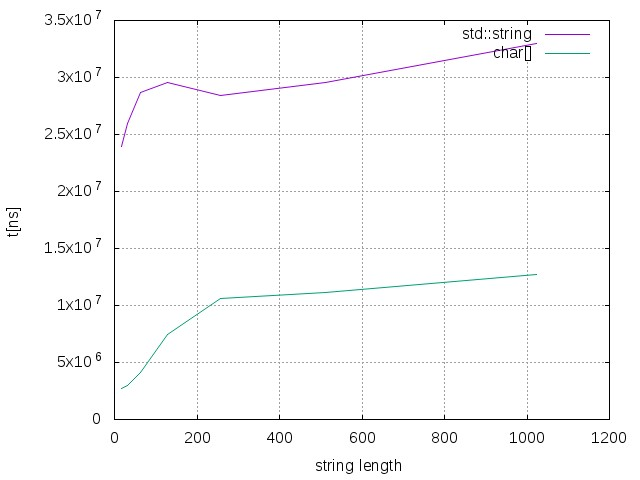
\includegraphics[width=\textwidth,height=0.8\textheight,keepaspectratio]
					{string_vs_raw_find.jpeg}
        \caption{find}
        \end{figure}
	\column{0.5\textwidth}
        \begin{figure}
        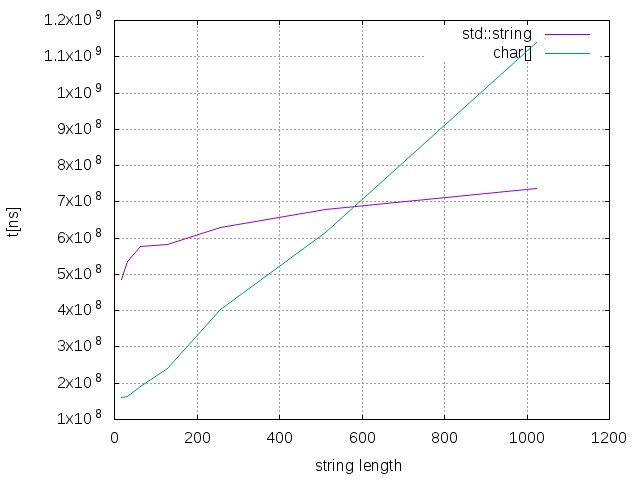
\includegraphics[width=\textwidth,height=0.8\textheight,keepaspectratio]
					{string_vs_raw_sort.jpeg}
        \caption{sort}
        \end{figure}
    \end{columns}
\end{frame}

\begin{frame}[fragile]
\frametitle{C-string vs \texttt{std::string}}
    \begin{onlyenv}<1-2>
    \begin{lstlisting}
        class WithCString
        {
            char mName[20];
        public:
            const char* name() const
            {
                return mName;
            }
        };
    \end{lstlisting}

    \begin{alertblock}{}<2>
        Returns raw string forcing user to use raw string functions.
    \end{alertblock}

    \end{onlyenv}
    
    \begin{onlyenv}<3-6>
    \begin{lstlisting}
        class WithCString
        {
            char mName[20];
        public:
            std::string name() const
            {
                return std::string{mName, 20};
            }
        };
    \end{lstlisting}

    \begin{alertblock}{}<4>
        Returns std::string but requires a new copy of the original string.
    \end{alertblock}
    \end{onlyenv}

    \hrulefill
    \begin{onlyenv}<5>
    \begin{lstlisting}
        WithCString str {"Johnny"};
        auto n = str.name().c_str();
        printf(%s, n);
    \end{lstlisting}
    \end{onlyenv}

    \begin{onlyenv}<6>
    \begin{lstlisting}
        WithCString str {"Johnny"};
        const char* n = `str.name()`.c_str();
        printf(%s, n);
    \end{lstlisting}

    \begin{alertblock}{Return from \texttt{str.name()} is a temporary object}<6>
        Pointer passed to printf is invalid.
    \end{alertblock}
    \end{onlyenv}

    \begin{onlyenv}<7-8>
    \begin{lstlisting}
        class WithCString
        {
            char mName[20];
        public:
            std::string_view name() const
            {
                return std::string_view{mName, 20};
            }
        };
    \end{lstlisting}

    \begin{block}{}<8>
        C++17 introduces \texttt{string\_view} class which can wrap an existing buffer into
        \texttt{string}-like object.
    \end{block}
    \end{onlyenv}
\end{frame}


\section{STL algorithms}

\begin{frame}
    \begin{center}
        STL algorithms
    \end{center}
\end{frame}

\begin{frame}
\frametitle{Motivation}
	\begin{itemize}
		\item Standard Library provides a wide variety of algorithms on containers which
			  don't get as much popularity as they deserve
		\pause
		\item Programmers tend to write their own raw loops to solve the same problems
		\pause
		\item Usually these are clumsy loops (often nested) with hard to understand control
			  flow
		\item The loops often are specific to only one container type
		\pause
		\item Sometimes these loops are not as efficient as they could be
	\end{itemize}
\end{frame}

\begin{frame}[fragile,t]
\frametitle {What does this code do?}
	\begin{lstlisting}
		std::vector<int> v1 = {1, 2, 3, 5, 8, 11, 13, 18};
		std::vector<int> v2 = {5, 7, 14, 18};
		std::vector<int> v3;
	\end{lstlisting}
	
	\begin{onlyenv}<1>
	\begin{lstlisting}
		for (auto it1 = v1.begin(), it2 = v2.begin(); it1 != v1.end();)
	    {
	        if (*it1 < *it2)
	        {
	            v3.push_back(*it1++);
	        }
	        else if (*it1 > *it2)
	        {
	            ++it2;
	        }
	        else
	        {
	            ++it1;
	            ++it2;
	        }
	    }
	\end{lstlisting}
	\end{onlyenv}
	
	\begin{onlyenv}<2>
	\begin{lstlisting}
	    std::set_difference(v1.begin(), v1.end(), v2.begin(), v2.end(),
                        std::back_inserter(v3));
	\end{lstlisting}
	\end{onlyenv}
	\begin{lstlisting}
		// What's in v3?
	\end{lstlisting}
\end{frame}

\begin{frame}[fragile]
\frametitle{\texttt{std::set\_difference}}
	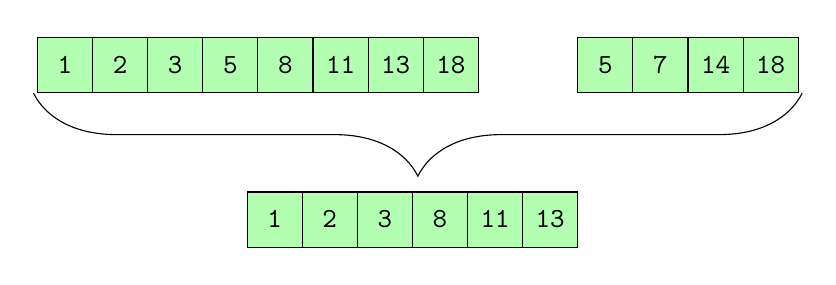
\begin{tikzpicture}[font=\ttfamily,
		vector/.style={matrix of nodes,nodes={draw, minimum size=7mm, fill=green!30},
		column sep=-\pgflinewidth, row sep=0.0mm, nodes in empty cells}]
		\tikzset{row 1/.style={nodes={fill=green!30}}}
		\matrix[vector] (v1){
				1& 2& 3& 5& 8& 11& 13& 18\\};
		
		\matrix[vector, right=of v1] (v2){
				5& 7& 14& 18\\};
		\matrix[vector, below=of v2, xshift=-3.5cm] (v3){
				1& 2& 3& 8& 11& 13\\};
		%\draw[->](v2) -- (v3);
		\draw[decorate,decoration={brace,mirror,amplitude=30pt}]([xshift=-4mm]v1-1-1.south) -- ([xshift=4mm]v2-1-4.south);
	\end{tikzpicture}
\end{frame}

\begin{frame}
\frametitle{Motivation}
	Avoid writing raw loops. \newline
	Learn STL algorithms and use them where applicable. \newline
	Combine multiple STL algorithms into more complex procedures.
\end{frame}

\begin{frame}[fragile]
\frametitle{Generate random string}
    \begin{lstlisting}
        std::string
        randomString(size_t n)
        {
            static std::random_device rd;
            std::default_random_engine re(rd());
            std::uniform_int_distribution<char> dist{33, 122};
            std::string s(n, '\0');
            std::generate(s.begin(), s.end(), [&re, &dist]() { return dist(re); });
            return s;
        }
    \end{lstlisting}
\end{frame}

\begin{frame}[fragile]
\frametitle{Check if two containers have same elements}
    \begin{onlyenv}<1>
    \begin{lstlisting}
        template <class Container>
        haveSameElements(Container c1, Container c2)
        {
            if (c1.size() != c2.size())
            {
                return false;
            }

            std::sort(c1.begin(), c1.end());
            std::sort(c2.begin(), c2.end());
            return c1 == c2;
        }
    \end{lstlisting}
    \end{onlyenv}

    \begin{onlyenv}<2>
    \begin{lstlisting}
        template <class Container>
        haveSameElements(const Container c1&, const Container& c2)
        {
            return std::is_permutation(c1.begin(), c1.end(), c2.begin());
        }
    \end{lstlisting}
    \end{onlyenv}
\end{frame}

\begin{frame}[fragile]
\frametitle{Remove duplicates}
    \begin{onlyenv}<1>
    \begin{lstlisting}
    template <typename T> void removeDuplicates (std::vector<T>& v)
    {
        if (v.size() > 1)
        {
            typename std::vector<T>::iterator it;
            std::set<T> seen;

            for (it = v.begin(); it != v.end();)
            {
                if (seen.find(*it) == seen.end())
                {
                    seen.insert(*it);
                    it ++;
                }
                else
                {
                    it = v.erase(it);
                }
            }
        }
    }
    \end{lstlisting}
    \end{onlyenv}
    \begin{onlyenv}<2>
    \begin{lstlisting}
    template <typename T> void removeDuplicates (std::vector<T>& v)
    {
        v.sort(v.begin(), v.end());
        v.erase(std::unique(v.begin(), v.end()), end());
    }
    \end{lstlisting}
    \end{onlyenv}
\end{frame}

\begin{frame}[fragile]
\frametitle{Find index}
    \begin{onlyenv}<1>
    \begin{lstlisting}
    template<typename T>
    int find(const std::vector<T>& v, const T& val)
    {
        int idx = 0;
        int found = false;
        for (const auto& x : v)
        {
            if (x == val)
            {
                found = true;
                break;
            }
            idx++;
        }
        return found ? idx : -1;
    }
    \end{lstlisting}
    \end{onlyenv}
    \begin{onlyenv}<2>
    \begin{lstlisting}
    template<typename T>
    int find(const std::vector<T>& v, const T& val)
    {
        auto it = std::find(v.begin(), v.end(), val);
        return it != v.end() ? std::distance(v.begin(), it) : -1;
    }
    \end{lstlisting}
    \end{onlyenv}
\end{frame}

\begin{frame}
\frametitle{Employee database}
\begin{itemize}
	\item Database storing basic information on employees
	\item Supports basic operations
	\begin{itemize}
		\item Insertion/Removal
		\item Look up
		\item Traversal
	\end{itemize}
	\item Optimized for look-ups and traversals at the cost of insertion and removal
	\item Goals
	\begin{itemize}
		\item Implement statistical algorithms with minimal or no usage of raw loops
	\end{itemize}
\end{itemize}
\end{frame}

\begin{frame}[fragile,t]
\frametitle{Employee database}
	\begin{lstlisting}
		enum class Profession
		{
		    ENGINEER,
		    DOCTOR,
		    LAWYER
		};
		
		struct EmployeeRecord
		{
		    std::string name;
		    Profession profession = Profession::ENGINEER;
		    int age                   = 0;
		    int salary                = 0;
		    uint64_t id               = 0;
		
		    EmployeeRecord() = default;
		    EmployeeRecord(std::string name, Profession profession, int age, int salary)
		        : name(std::move(name)), profession(profession), age(age), salary(salary)
		    {
		    }
		};

	\end{lstlisting}
\end{frame}

\begin{frame}[fragile,t]
\frametitle{Employee database}
\setbeamercovered{transparent}
	\begin{lstlisting}
		class EmployeesDb
		{	|\onslide<1>|
		    using Collection = std::vector<EmployeeRecord>;
		    using NameLookup = std::unordered_map<std::string, uint64_t>;
		    using IdLookup   = std::unordered_map<uint64_t, size_t>;
		
		    Collection mEmployees;
		    NameLookup mNameLookup;
		    IdLookup mIdLookup;
		|\onslide<1->|
		public: |\onslide<0>|
		    using Iterator = Collection::const_iterator;
			
		    EmployeesDb() = default;
		    EmployeesDb(std::vector<EmployeeRecord> employees);
		    ~EmployeesDb() = default;
			
		    uint64_t insert(EmployeeRecord data);
		    void remove(const std::string& name);
		    void remove(uint64_t id);
		    Iterator find(uint64_t id) const;
		    Iterator find(const std::string& name) const;
		    size_t size() const;
		    Iterator begin() const;
		    Iterator end() const;
	
		private:
		    void generateIdLookup();
		    void generateNameLookup(); |\onslide<1->|
		};
	\end{lstlisting}
\end{frame}

\begin{frame}[fragile]
\frametitle{Employee database}
	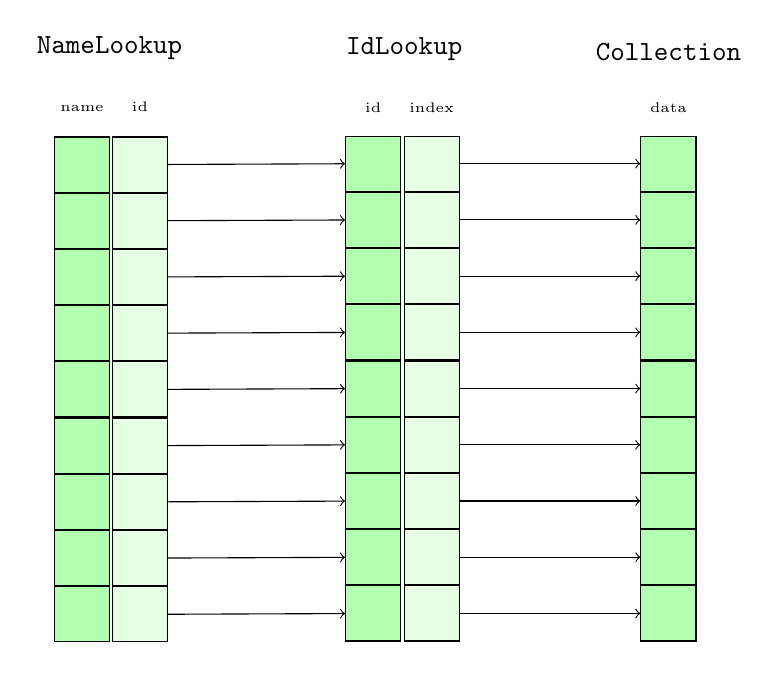
\begin{tikzpicture}[font=\ttfamily,
		map/.style={matrix of nodes,nodes={draw, minimum size=7mm, fill=green!30},
		column sep=-\pgflinewidth, row sep=0.0mm, nodes in empty cells, font=\tiny,
	    column 2/.style={nodes={draw, fill=green!10}},
		row 1/.style={nodes={draw=none, fill=none}}},
		vector/.style={matrix of nodes,nodes={draw, minimum size=7mm, fill=green!30},
		column sep=-\pgflinewidth, row sep=0.0mm, nodes in empty cells, font=\tiny,
		row 1/.style={nodes={draw=none, fill=none}}}]
		
		\matrix[map, label={NameLookup}] (nameMap) {
		name & id \\ & \\ & \\ & \\ & \\ & \\ & \\ & \\ & \\ & \\};
		\matrix[map, right=2cm of nameMap, label={IdLookup}] (idMap) {
		id & index \\ & \\ & \\ & \\ & \\ & \\ & \\ & \\ & \\ & \\};
		\matrix[vector, right=2cm of idMap, label={Collection}] (vec) {
		data \\ \\ \\ \\ \\ \\ \\ \\ \\ \\};

		\foreach \i in {2, ..., 10}{
			\draw[->](nameMap-\i-2) -- (idMap-\i-1);
		}
		\foreach \i in {2, ..., 10}{
			\draw[->](idMap-\i-2) -- (vec-\i-1);
		}
	\end{tikzpicture}
\end{frame}

\begin{frame}
\frametitle{Iteration efficiency}
\framesubtitle{Cache locality matters}
	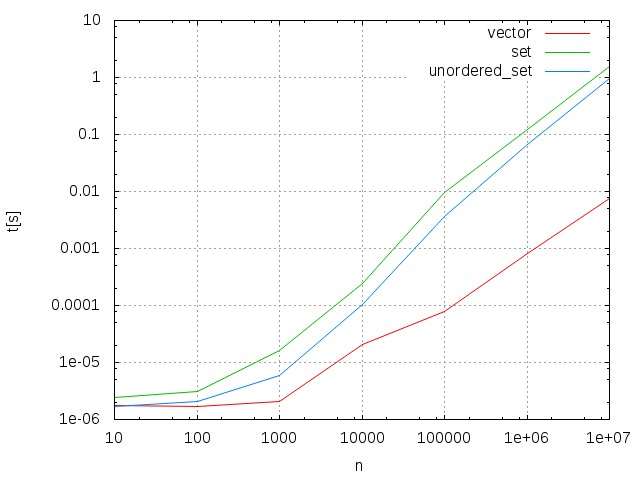
\includegraphics[width=\textwidth,height=0.8\textheight,keepaspectratio]
					{col_iter.jpeg}
\end{frame}

\begin{frame}[fragile,t]
\frametitle{Employee database}
\setbeamercovered{transparent}
	\begin{lstlisting}
		class EmployeesDb
		{	|\onslide<1>|
		    using Collection = std::vector<EmployeeRecord>;
		    using NameLookup = std::unordered_map<std::string, uint64_t>;
		    using IdLookup   = std::unordered_map<uint64_t, size_t>;
		
		    Collection mEmployees;
		    NameLookup mNameLookup;
		    IdLookup mIdLookup;
		|\onslide<1->|
		public: |\onslide<4>|
		    using Iterator = Collection::const_iterator;
			|\onslide<2>|
		    EmployeesDb() = default;
		    EmployeesDb(std::vector<EmployeeRecord> employees);
		    ~EmployeesDb() = default;
			|\onslide<3>|
		    uint64_t insert(EmployeeRecord data);
		    void remove(const std::string& name);
		    void remove(uint64_t id); |\onslide<4>|
		    Iterator find(uint64_t id) const;
		    Iterator find(const std::string& name) const; |\onslide<5>|
		    size_t size() const;
		    Iterator begin() const;
		    Iterator end() const;
			|\onslide<6>|
		private:
		    void generateIdLookup();
		    void generateNameLookup(); |\onslide<1->|
		};
	\end{lstlisting}
\end{frame}

\begin{frame}[fragile]
\frametitle{Employees database}
\setbeamercovered{transparent}
	\begin{lstlisting}
		EmployeesDb::EmployeesDb(std::vector<EmployeeRecord> employees)
	    	: mEmployees(std::move(employees))
		{
		    // Collection internally partitioned by Profession|\onslide<1>|
		    auto it =
		        std::partition(mEmployees.begin(), mEmployees.end(), [](const EmployeeRecord& e) {
		            return e.profession == Profession::ENGINEER;
		        });|\onslide<0>|
		    std::partition(it, mEmployees.end(), [](const EmployeeRecord& e) {
		        return e.profession == Profession::DOCTOR;
		
		    });
			
		    generateNameLookup();
		    generateIdLookup();|\onslide<1>|
		}
	\end{lstlisting}
\end{frame}
	
\begin{frame}[fragile]
\frametitle{\texttt{std::partition}}
	\newcommand{\element}[2]{
		\foreach \r in {#1} {%
  			\globaldefs=1\relax
  			\tikzset{column \r/.style={nodes={fill=#2}}}
		}%
	}

	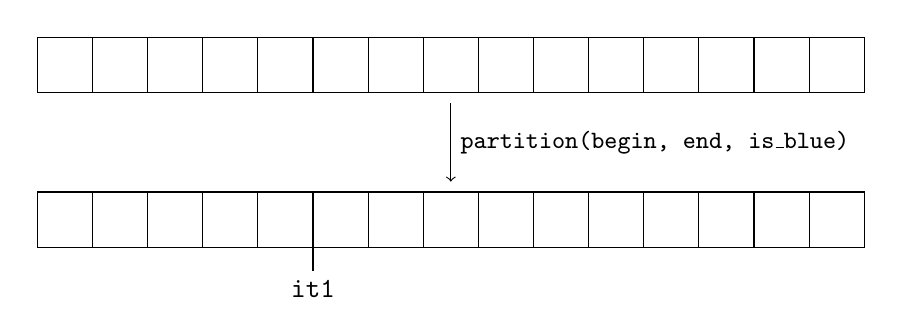
\begin{tikzpicture}[font=\ttfamily,
		vector/.style={matrix of nodes,nodes={draw, minimum size=7mm},
		column sep=-\pgflinewidth, row sep=0.0mm, nodes in empty cells}]
	
		\element{1,3,7,11,15}{blue!30}
		\element{2,5,6,12}{red!30}
		\element{4,8,9,10,13,14}{green!30}
		\matrix[vector] (v1){
			& & & & & & & & & & & & & &\\};
		
		\element{1,2,3,4,5}{blue!30}
		\element{6,7,12,15}{red!30}
		\element{8,9,10,11,13,14}{green!30}
		\matrix[vector, below=of v1] (v2){
			& & & & & & & & & & & & & &\\};
			
		\draw[->](v1) -- (v2) node [midway, right, font=\small] 
			{\texttt{partition(begin, end, is\_blue)}};	
		\draw ([xshift=-3.5mm]v2-1-6.south)--++(90:-3mm) node [below] {it1};
	\end{tikzpicture}
\end{frame}

\begin{frame}[fragile]
\frametitle{Employees database}
\setbeamercovered{transparent}
	\begin{lstlisting}
		EmployeesDb::EmployeesDb(std::vector<EmployeeRecord> employees)
	    	: mEmployees(std::move(employees))
		{
		    // Collection internally partitioned by Profession
		    auto it =
		        std::partition(mEmployees.begin(), mEmployees.end(), [](const EmployeeRecord& e) {
		            return e.profession == Profession::ENGINEER;
		        });
		    std::partition(it, mEmployees.end(), [](const EmployeeRecord& e) {
		        return e.profession == Profession::DOCTOR;
		
		    });

		    generateNameLookup();
		    generateIdLookup();|\onslide<1->|
		}
	\end{lstlisting}
\end{frame}

\begin{frame}[fragile]
\frametitle{\texttt{std::partition}}
	\newcommand{\element}[2]{
		\foreach \r in {#1} {%
  			\globaldefs=1\relax
  			\tikzset{column \r/.style={nodes={fill=#2}}}
		}%
	}

	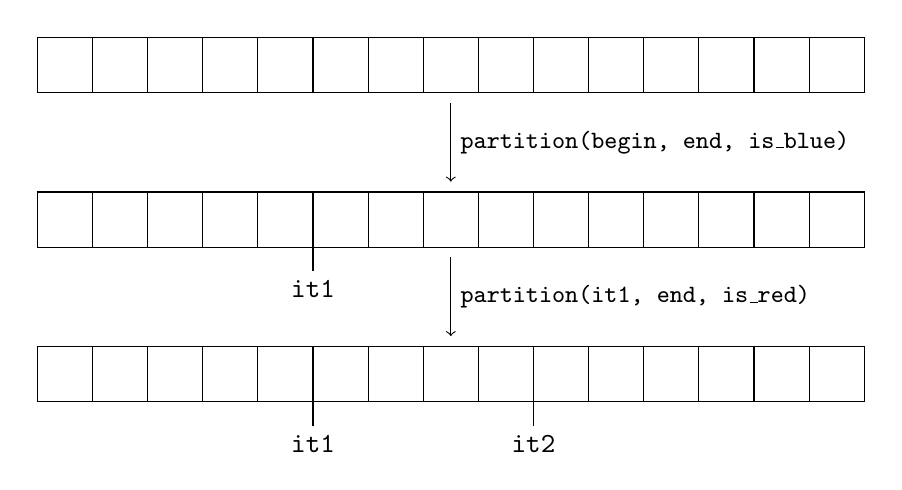
\begin{tikzpicture}[font=\ttfamily,
		vector/.style={matrix of nodes,nodes={draw, minimum size=7mm},
		column sep=-\pgflinewidth, row sep=0.0mm, nodes in empty cells}]
	
		\element{1,3,7,11,15}{blue!30}
		\element{2,5,6,12}{red!30}
		\element{4,8,9,10,13,14}{green!30}
		\matrix[vector] (v1){
			& & & & & & & & & & & & & &\\};
		
		\element{1,2,3,4,5}{blue!30}
		\element{6,7,12,15}{red!30}
		\element{8,9,10,11,13,14}{green!30}
		\matrix[vector, below=of v1] (v2){
			& & & & & & & & & & & & & &\\};
		
		\element{1,2,3,4,5}{blue!30}
		\element{6,7,8,9}{red!30}
		\element{10,11,12,13,14,15}{green!30}
		\matrix[vector, below=of v2] (v3){
			& & & & & & & & & & & & & &\\};
			
		\draw[->](v1) -- (v2) node [midway, right, font=\small] 
			{\texttt{partition(begin, end, is\_blue)}};	
		\draw ([xshift=-3.5mm]v2-1-6.south)--++(90:-3mm) node [below] {it1};
		\draw[->](v2) -- (v3) node [midway, right, font=\small] 
			{\texttt{partition(it1, end, is\_red)}};
		\draw ([xshift=-3.5mm]v3-1-6.south)--++(90:-3mm) node [below] {it1};
		\draw ([xshift=-3.5mm]v3-1-10.south)--++(90:-3mm) node [below] {it2};
	\end{tikzpicture}
\end{frame}

\begin{frame}[fragile]
\frametitle{Employees database}
\framesubtitle{range}
\setbeamercovered{transparent}
	\begin{lstlisting}
		std::pair<EmployeesDb::Iterator, EmployeesDb::Iterator>
		range(const EmployeesDb& db, Profession profession)
		{|\onslide<1->|
		    auto compPos1 = [](const EmployeeRecord& e, Profession pos) {
		        return e.profession < pos;
		    };
		|\onslide<2->|
		    auto compPos2 = [](Profession pos, const EmployeeRecord& e) {
		        return pos < e.profession;
		    };
		|\onslide<1->|
		    auto begin = std::lower_bound(db.begin(), db.end(), profession, compPos1);|\onslide<2->|
		    auto end   = std::upper_bound(db.begin(), db.end(), profession, compPos2);|\onslide<2->|
		    return {begin, end};|\onslide<1->|
		}
	\end{lstlisting}
\end{frame}	

\begin{frame}[fragile]
\frametitle{\texttt{std::lower\_bound} and \texttt{std::upper\_bound}}

	\newcommand{\element}[2]{
		\foreach \r in {#1} {%
  			\globaldefs=1\relax
  			\tikzset{column \r/.style={nodes={fill=#2}}}
		}%
	}
	
	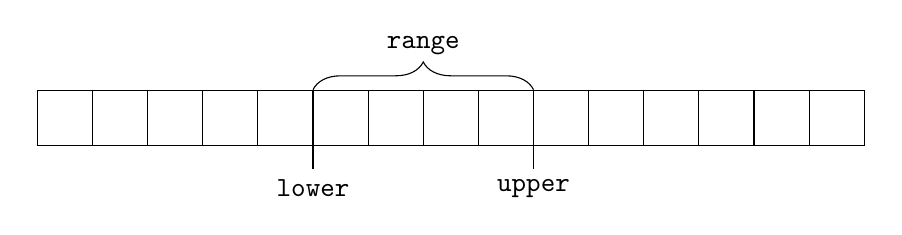
\begin{tikzpicture}[font=\ttfamily,
		vector/.style={matrix of nodes,nodes={draw, minimum size=7mm},
		column sep=-\pgflinewidth, row sep=0.0mm, nodes in empty cells}]
		
		\element{1,2,3,4,5}{blue!30}
		\element{6,7,8,9}{red!30}
		\element{10,11,12,13,14,15}{green!30}
		\matrix[vector] (v1){
			& & & & & & & & & & & & & &\\};
			
		\draw ([xshift=-3.5mm]v1-1-6.south)--++(90:-3mm) node [below] {lower};
		\draw ([xshift=-3.5mm]v1-1-10.south)--++(90:-3mm) node [below] {upper};
		\draw[decorate,decoration={brace,amplitude=10pt}]([xshift=-3.5mm]v1-1-6.north) -- ([xshift=-3.5mm]v1-1-10.north) node [midway, above, yshift=9pt] {range};
	\end{tikzpicture}
\end{frame}

\begin{frame}[fragile]
\frametitle{Employees database}
\framesubtitle{Min and Max}
\setbeamercovered{transparent}
	\begin{lstlisting}
		std::pair<EmployeesRecord, EmployeesRecord>
		minMaxSalaryPerPosition(const EmployeesDb& db, Profession profession)
		{
		    auto r = range(db, profession);
		    minMax std::minmax_element(r.first, r.second,
		                               [](const EmployeeRecord& e1, const EmployeeRecord& e2) {
		                                   return e1.salary < e2.salary;
		                               });
            return {*minMax.first, *minMax.second};
		}
	\end{lstlisting}
\end{frame}	

\begin{frame}[fragile]
\frametitle{Employees database}
\framesubtitle{\texttt{Average}}
\setbeamercovered{transparent}
	\begin{lstlisting}
		int
		avgSalaryPerPosition(const EmployeesDb& db, Profession profession)
		{|\onslide<1>|
		    auto r = range(db, profession);
		    auto totalSalary =
		        std::accumulate(r.first, r.second, uint64_t{0},
		                        [](uint64_t s, const EmployeeRecord& e) { return s + e.salary; });|\onslide<0>|
		    auto noOfEmployees = std::distance(r.first, r.second);
		    return totalSalary / noOfEmployees;|\onslide<1>|
		}
	\end{lstlisting}
\end{frame}

\begin{frame}[fragile]
\frametitle{\texttt{std::accumulate}}

	\newcommand{\element}[2]{
		\foreach \r in {#1} {%
  			\globaldefs=1\relax
  			\tikzset{column \r/.style={nodes={fill=#2}}}
		}%
	}
	
	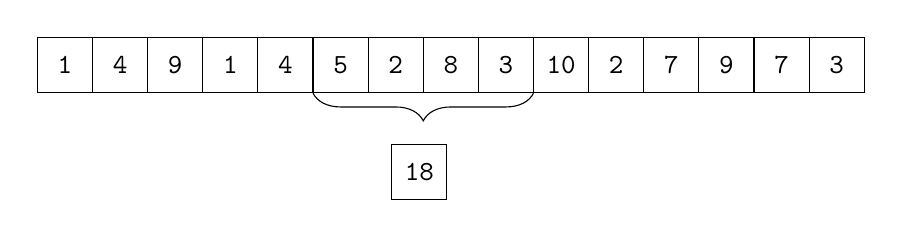
\begin{tikzpicture}[font=\ttfamily,
		vector/.style={matrix of nodes,nodes={draw, minimum size=7mm},
		column sep=-\pgflinewidth, row sep=0.0mm, nodes in empty cells}]
		
		\element{1,2,3,4,5}{blue!30}
		\element{6,7,8,9}{red!30}
		\element{10,11,12,13,14,15}{green!30}
		\matrix[vector] (v1){
		 1 &4 &9 &1 &4 &5 &2 &8 &3 &10 &2 &7 &9 &7 &3\\};
		 \element{1}{red!30}
		\matrix[vector, below=of v1, yshift=6mm,xshift=-4mm] (v2){
		 18\\};
		 
		 \draw[decorate,decoration={brace,mirror,amplitude=10pt}]([xshift=-3.5mm]v1-1-6.south) -- ([xshift=-3.5mm]v1-1-10.south);
	\end{tikzpicture}
\end{frame}

\begin{frame}[fragile]
\frametitle{Employees database}
\framesubtitle{Average}
\setbeamercovered{transparent}
	\begin{lstlisting}
		int
		avgSalaryPerPosition(const EmployeesDb& db, Profession profession)
		{|\onslide<1->|
		    auto r = range(db, profession);
		    auto totalSalary =
		        std::accumulate(r.first, r.second, uint64_t{0},
		                        [](uint64_t s, const EmployeeRecord& e) { return s + e.salary; });|\onslide<2->|
		    auto noOfEmployees = std::distance(r.first, r.second);
		    return totalSalary / noOfEmployees;|\onslide<1->|
		}
	\end{lstlisting}
\end{frame}

\begin{frame}[fragile]
\frametitle{\texttt{std::distance}}

	\newcommand{\element}[2]{
		\foreach \r in {#1} {%
  			\globaldefs=1\relax
  			\tikzset{column \r/.style={nodes={fill=#2}}}
		}%
	}
	
	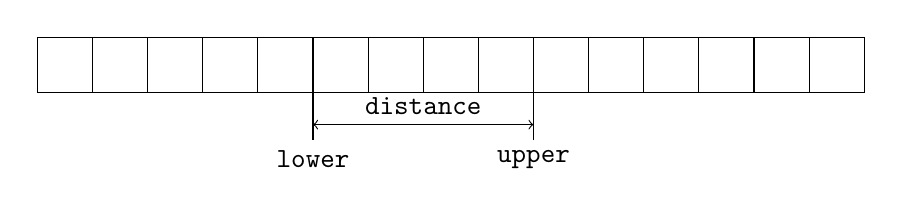
\begin{tikzpicture}[font=\ttfamily,
		vector/.style={matrix of nodes,nodes={draw, minimum size=7mm},
		column sep=-\pgflinewidth, row sep=0.0mm, nodes in empty cells}]
		
		\element{1,2,3,4,5}{blue!30}
		\element{6,7,8,9}{red!30}
		\element{10,11,12,13,14,15}{green!30}
		\matrix[vector] (v1){
			& & & & & & & & & & & & & &\\};
			
		\draw ([xshift=-3.5mm]v1-1-6.south)--++(90:-6mm) node [below] (lower) {lower};
		\draw ([xshift=-3.5mm]v1-1-10.south)--++(90:-6mm) node [below] (upper) {upper};
		\draw[<->]([yshift=-4mm,xshift=-3.5mm]v1-1-6.south) -- node [above] {distance} ([yshift=-4mm,xshift=-3.5mm]v1-1-10.south) ;
	\end{tikzpicture}
\end{frame}

\begin{frame}[fragile]
\frametitle{Employees database}
\framesubtitle{Median}
\setbeamercovered{transparent}
	\begin{lstlisting}
		int
		medianSalaryPerPosition(const EmployeesDb& db, Profession profession)
		{
		    auto r             = range(db, profession);
		    auto noOfEmployees = std::distance(r.first, r.second);
		    std::vector<int> salaries(noOfEmployees);
		    std::transform(r.first, r.second, salaries.begin(),
		                   [](const EmployeeRecord& e) { return e.salary; });
			|\onslide<0>|
		    std::nth_element(salaries.begin(), salaries.begin() + salaries.size() / 2,
		                     salaries.end());
		    return salaries[salaries.size() / 2];|\onslide<1->|
		}
	\end{lstlisting}
\end{frame}

\begin{frame}[fragile]
\frametitle{\texttt{std::transform}}
	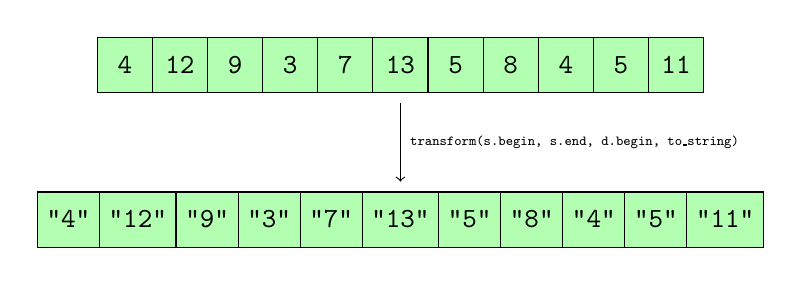
\begin{tikzpicture}[font=\ttfamily,
		vector/.style={matrix of nodes,nodes={draw, minimum size=7mm, fill=green!30},
		column sep=-\pgflinewidth, row sep=0.0mm, nodes in empty cells}]
		\tikzset{row 1/.style={nodes={fill=green!30}}}
		\matrix[vector] (v1){
				4& 12& 9& 3& 7& 13& 5& 8& 4& 5& 11\\};
		\tikzset{row 1 /.style={nodes={fill=blue!30}}}
		\matrix[vector, below=of v1] (v2){
				"4"& "12"& "9"& "3"& "7"& "13"& "5"& "8"& "4"& "5"& "11"\\};
		\draw[->](v1) -- (v2) node [midway, right, font=\tiny] 
			{\texttt{transform(s.begin, s.end, d.begin, to\_string)}};
	\end{tikzpicture}
\end{frame}

\begin{frame}[fragile]
\frametitle{Employees database}
\framesubtitle{Median}
\setbeamercovered{transparent}
	\begin{lstlisting}
		int
		medianSalaryPerPosition(const EmployeesDb& db, Profession profession)
		{|\onslide<0>|
		    auto r             = range(db, profession);
		    auto noOfEmployees = std::distance(r.first, r.second);
		    std::vector<int> salaries(noOfEmployees);
		    std::transform(r.first, r.second, salaries.begin(),
		                   [](const EmployeeRecord& e) { return e.salary; });
			|\onslide<1>|
		    std::nth_element(salaries.begin(), salaries.begin() + salaries.size() / 2,
		                     salaries.end());
		    return salaries[salaries.size() / 2];|\onslide<1->|
		 }
	\end{lstlisting}
\end{frame}	

\begin{frame}[fragile]
\frametitle{\texttt{std::nth\_element}}
	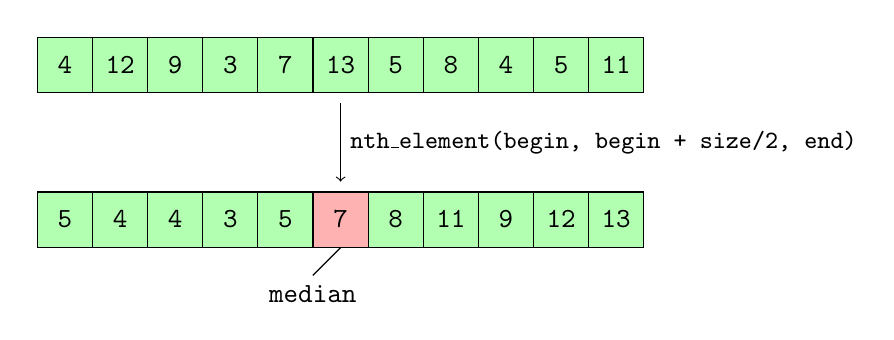
\begin{tikzpicture}[font=\ttfamily,
		vector/.style={matrix of nodes,nodes={draw, minimum size=7mm, fill=green!30},
		column sep=-\pgflinewidth, row sep=0.0mm, nodes in empty cells}]
		\tikzset{row 1/.style={nodes={fill=green!30}}}
		\matrix[vector] (v1){
				4& 12& 9& 3& 7& 13& 5& 8& 4& 5& 11\\};
		\tikzset{row 1 column 6/.style={nodes={fill=red!30}}}
		\matrix[vector, below=of v1] (v2){
				5& 4& 4& 3& 5& 7& 8& 11& 9& 12& 13\\};
		\draw[->](v1) -- (v2) node [midway, right, font=\small] 
			{\texttt{nth\_element(begin, begin + size/2, end)}};
		\pause
		\draw (v2-1-6.south)--++(45:-5mm) node [below] {median};
	\end{tikzpicture}
\end{frame}	

\begin{frame}[fragile]
\frametitle{Employees database}
\framesubtitle{Median}
\setbeamercovered{transparent}
	\begin{lstlisting}
		int
		medianSalaryPerPosition(const EmployeesDb& db, Profession profession)
		{
		    auto r             = range(db, profession);
		    auto noOfEmployees = std::distance(r.first, r.second);
		    std::vector<int> salaries(noOfEmployees);
		    std::transform(r.first, r.second, salaries.begin(),
		                   [](const EmployeeRecord& e) { return e.salary; });
			|\onslide<1>|
		    std::nth_element(salaries.begin(), salaries.begin() + salaries.size() / 2,
		                     salaries.end());
		    return salaries[salaries.size() / 2];
		 }
	\end{lstlisting}
\end{frame}

\begin{frame}[fragile]
\frametitle{Employees database}
\framesubtitle{Top N}
\setbeamercovered{transparent}
	\begin{lstlisting}
		std::vector<EmployeesDb::Iterator>
		topNSalariesPerPosition(const EmployeesDb& db, Profession profession, int n)
		{
		    auto r             = range(db, profession);
		    auto noOfEmployees = std::distance(r.first, r.second);
		
		    struct Helper
		    {
		        uint64_t id;
		        int salary;
		    };
			|\onslide<2->|		
		    std::vector<Helper> data(noOfEmployees);
		    std::transform(r.first, r.second, data.begin(), [](const EmployeeRecord& e) {
		        return Helper{e.id, e.salary};
		    });
			|\onslide<3->|
		    std::nth_element(
		        data.begin(), data.end() - n, data.end(),
		        [](const Helper& e1, const Helper& e2) { return e1.salary < e2.salary; });
			|\onslide<0>|
		    std::sort(data.end() - n, data.end(),
		              [](const Helper& e1, const Helper& e2) { return e1.salary > e2.salary; });
			|\onslide<0>|
		    std::vector<EmployeesDb::Iterator> employeesTopN(n);
		    std::transform(data.end() - n, data.end(), employeesTopN.begin(),
		                   [&db](const Helper& e) { return db.find(e.id); });
		    return employeesTopN;|\onslide<1->|
		}
	\end{lstlisting}
\end{frame}

\begin{frame}[fragile]
\frametitle{\texttt{std::nth\_element}}
	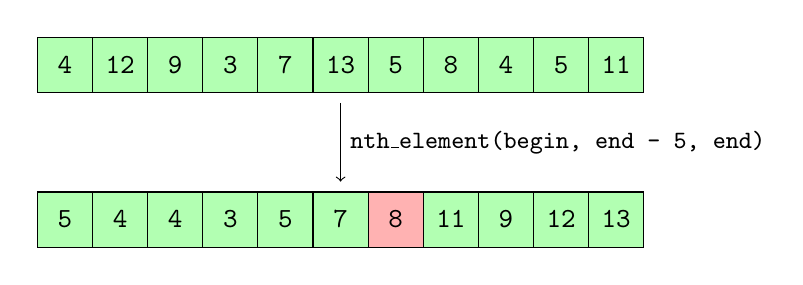
\begin{tikzpicture}[font=\ttfamily,
		vector/.style={matrix of nodes,nodes={draw, minimum size=7mm, fill=green!30},
		column sep=-\pgflinewidth, row sep=0.0mm, nodes in empty cells}]
		\tikzset{row 1/.style={nodes={fill=green!30}}}
		\matrix[vector] (v1){
				4& 12& 9& 3& 7& 13& 5& 8& 4& 5& 11\\};
		\tikzset{row 1 column 7/.style={nodes={fill=red!30}}}
		\matrix[vector, below=of v1] (v2){
				5& 4& 4& 3& 5& 7& 8& 11& 9& 12& 13\\};
		\draw[->](v1) -- (v2) node [midway, right, font=\small] 
			{\texttt{nth\_element(begin, end - 5, end)}};
	\end{tikzpicture}
\end{frame}	

\begin{frame}[fragile]
\frametitle{Employees database}
\framesubtitle{Top N}
\setbeamercovered{transparent}
	\begin{lstlisting}
		std::vector<EmployeesDb::Iterator>
		topNSalariesPerPosition(const EmployeesDb& db, Profession profession, int n)
		{|\onslide<0>|
		    auto r             = range(db, profession);
		    auto noOfEmployees = std::distance(r.first, r.second);
		
		    struct Helper
		    {
		        uint64_t id;
		        int salary;
		    };
					
		    std::vector<Helper> data(noOfEmployees);
		    std::transform(r.first, r.second, data.begin(), [](const EmployeeRecord& e) {
		        return Helper{e.id, e.salary};
		    });
			|\onslide<1-2>|
		    auto fSalaryComp = [](const Helper& e1, const Helper& e2) {
        		return e1.salary < e2.salary;
    		};
    		
			std::nth_element(data.begin(), data.end() - n, data.end(), fSalaryComp);
			|\onslide<2>|
    		std::sort(data.end() - n, data.end(), fSalaryComp);

		    std::vector<EmployeesDb::Iterator> employeesTopN(n);
		    std::transform(data.rbegin(), data.rbegin() + n, employeesTopN.begin(),
                   [&db](const Helper& e) { return db.find(e.id); });
		    return employeesTopN;|\onslide<1->|
		}
	\end{lstlisting}
\end{frame}

\begin{frame}[fragile]
\frametitle{\texttt{std::nth\_element}}
	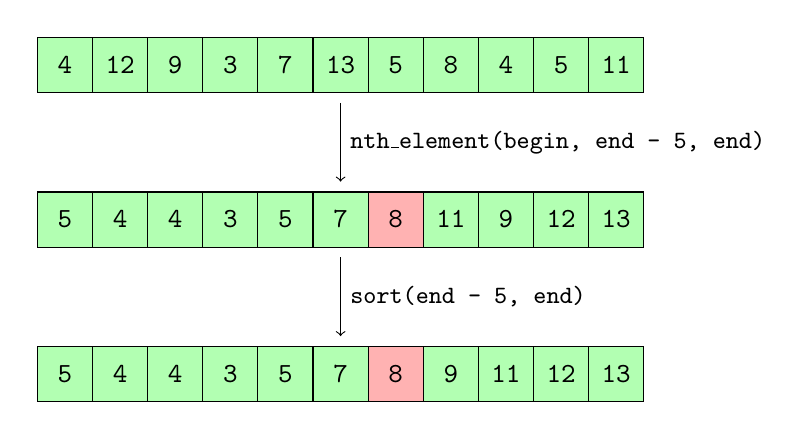
\begin{tikzpicture}[font=\ttfamily,
		vector/.style={matrix of nodes,nodes={draw, minimum size=7mm, fill=green!30},
		column sep=-\pgflinewidth, row sep=0.0mm, nodes in empty cells}]
		\tikzset{row 1/.style={nodes={fill=green!30}}}
		\matrix[vector] (v1){
				4& 12& 9& 3& 7& 13& 5& 8& 4& 5& 11\\};
		\tikzset{row 1 column 7/.style={nodes={fill=red!30}}}
		\matrix[vector, below=of v1] (v2){
				5& 4& 4& 3& 5& 7& 8& 11& 9& 12& 13\\};
		\matrix[vector, below=of v2] (v3){
				5& 4& 4& 3& 5& 7& 8& 9& 11& 12& 13\\};
		\draw[->](v1) -- (v2) node [midway, right, font=\small] 
			{\texttt{nth\_element(begin, end - 5, end)}};
		\draw[->](v2) -- (v3) node [midway, right, font=\small] 
			{\texttt{sort(end - 5, end)}};
		
	\end{tikzpicture}
\end{frame}	

\begin{frame}[fragile]
\frametitle{Employees database}
\framesubtitle{Top N}
\setbeamercovered{transparent}
	\begin{lstlisting}
		std::vector<EmployeesRecord>
		topNSalariesPerPosition(const EmployeesDb& db, Profession profession, int n)
		{|\onslide<0>|
		    auto r             = range(db, profession);
		    auto noOfEmployees = std::distance(r.first, r.second);
		
		    struct Helper
		    {
		        uint64_t id;
		        int salary;
		    };
					
		    std::vector<Helper> data(noOfEmployees);
		    std::transform(r.first, r.second, data.begin(), [](const EmployeeRecord& e) {
		        return Helper{e.id, e.salary};
		    });
			
		    auto fSalaryComp = [](const Helper& e1, const Helper& e2) {
        		return e1.salary < e2.salary;
    		};
    		
			std::nth_element(data.begin(), data.end() - n, data.end(), fSalaryComp);
			
    		std::sort(data.end() - n, data.end(), fSalaryComp);
			|\onslide<1>|
		    std::vector<EmployeesRecord> employeesTopN(n);
		    std::transform(data.rbegin(), data.rbegin() + n, employeesTopN.begin(),
                   [&db](const Helper& e) { return *db.find(e.id); });
		    return employeesTopN;|\onslide<1->|
		}
	\end{lstlisting}
\end{frame}

\begin{frame}[fragile]
\frametitle{Employees database}
\framesubtitle{Average}
\setbeamercovered{transparent}
	\begin{lstlisting}
		int
		avgSalaryPerAgeRange(const EmployeesDb& db, std::pair<int, int> ageRange)
		{
		    struct Helper
		    {
		        int age;
		        int salary;
		    };
		
		    std::vector<Helper> data(db.size());
		    std::transform(db.begin(), db.end(), data.begin(), [](const EmployeeRecord& e) {
		        return Helper{e.age, e.salary};
		    });
			|\onslide<2->|	
		    auto it = std::partition(data.begin(), data.end(), [&ageRange](const Helper& e) {
		        return e.age >= ageRange.first && e.age <= ageRange.second;
		    });
			|\onslide<3->|
		    auto totalSalary =
		        std::accumulate(data.begin(), it, uint64_t{0},
		                        [](uint64_t s, const Helper& e) { return s + e.salary; });
		    auto noOfEmployees = std::distance(data.begin(), it);
		    return totalSalary / noOfEmployees;
		|\onslide<1->|}
	\end{lstlisting}
\end{frame}

\begin{frame}
\frametitle{Algorithm efficiency}
	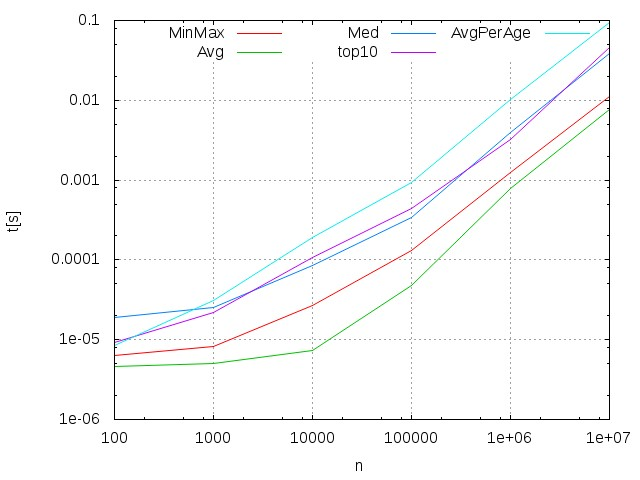
\includegraphics[width=\textwidth,height=0.8\textheight,keepaspectratio]
					{perf.jpeg}
\end{frame}

\begin{frame}[fragile,t]
\frametitle{Parallel computing}

	\begin{lstlisting}
		EmployeesDb db(emps);	
	\end{lstlisting}
	\begin{onlyenv}<1>
	\begin{lstlisting}
		auto s1 = avgSalaryPerAgeRange(db, {31, 35});
		auto s2 = avgSalaryPerAgeRange(db, {36, 40});
		auto s3 = avgSalaryPerAgeRange(db, {41, 45});
		auto s4 = avgSalaryPerAgeRange(db, {46, 50});
		auto s5 = avgSalaryPerAgeRange(db, {51, 55});
		auto s6 = avgSalaryPerAgeRange(db, {56, 60});
	\end{lstlisting}
	\end{onlyenv}
	
	\begin{onlyenv}<2>
	\begin{lstlisting}
		auto s1 = std::async(std::launch::async, avgSalaryPerAgeRange, std::cref(db),
                                 std::make_pair(31, 35));
		auto s2 = std::async(std::launch::async, avgSalaryPerAgeRange, std::cref(db),
                                 std::make_pair(36, 40));
        auto s3 = std::async(std::launch::async, avgSalaryPerAgeRange, std::cref(db),
                                 std::make_pair(41, 45));
        auto s4 = std::async(std::launch::async, avgSalaryPerAgeRange, std::cref(db),
                                 std::make_pair(46, 50));
        auto s5 = std::async(std::launch::async, avgSalaryPerAgeRange, std::cref(db),
                                 std::make_pair(51, 55));
        auto s6 = std::async(std::launch::async, avgSalaryPerAgeRange, std::cref(db),
                                 std::make_pair(56, 60));

        s1.wait();
        s2.wait();
        s3.wait();
        s4.wait();
        s5.wait();
        s6.wait();
	\end{lstlisting}
	\end{onlyenv}
\end{frame}

\begin{frame}
\frametitle{Parallel computing}
	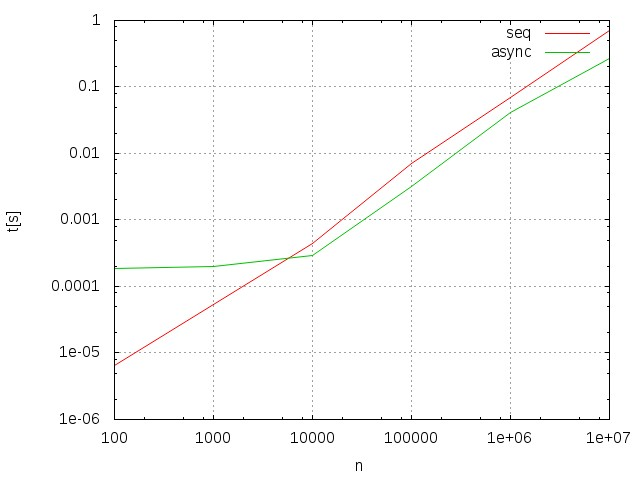
\includegraphics[width=\textwidth,height=0.8\textheight,keepaspectratio]
					{async.jpeg}
\end{frame}

\section{Conditional compilation}

\begin{frame}
    \begin{center}
        Conditional compilation.
    \end{center}
\end{frame}

\begin{frame}
\frametitle{Motivation}
    \begin{itemize}
        \item Quite often implementation has to consider platform specific details or idiosyncrasies
        \item The implementation then combines code which is platform agnostic and platform specific
        \item It is still common practice to pollute common implementation with platform specific details
              by using C-style \texttt{\#ifdef} macros
        \item That leads to so called "spaghetti code" which becomes hard to maintain
    \end{itemize}
\end{frame}

\begin{frame}[fragile,t]
    \begin{onlyenv}<1>
    \begin{lstlisting}
        void f(const X* x, const Y* y)
        {
            //common code

        #if defined(PRODUCT_A)
            // Product A code
        #elif defined(PRODUCT_B)
            // Product B code
        #elif defined(PRODUCT_C)
            // Product C code
        #endif

            // more common code
        }
    \end{lstlisting}
    \end{onlyenv}

    \begin{onlyenv}<2>
    \begin{lstlisting}
        void g(const X* x)
        {
        #if defined(PRODUCT_A)
            // Product A code
        #elif defined(PRODUCT_B)
            // Product B code
        #elif defined(PRODUCT_C)
            // Product C code
        #endif
        }

        void f(const X* x, const Y* y)
        {
            //common code
            g(x);
            //more common code
        }
    \end{lstlisting}
    \end{onlyenv}

    \begin{onlyenv}<3>
    \begin{lstlisting}
        void g_a(const X* x){//Product A code}
        void g_b(const X* x){//Product B code}
        void g_c(const X* x){//Product C code}
        
        void g(const X* x)
        {
        #if defined(PRODUCT_A)
            g_a(x);
        #elif defined(PRODUCT_B)
            g_b(x);
        #elif defined(PRODUCT_C)
            g_c(x);
        #endif
        }

        void f(const X* x, const Y* y)
        {
            //common code
            g(x);
            //more common code
        }

    \end{lstlisting}
    \end{onlyenv}
    
    \begin{onlyenv}<4>
    \begin{lstlisting}
        struct Product_A {};
        struct Product_B {};
        struct Product_C {};

        void g(const X* x, Product_A){//Product A code}
        void g(const X* x, Product_B){//Product B code}
        void g(const X* x, Product_C){//Product C code}
        
        void g(const X* x)
        {
        #if defined(PRODUCT_A)
            g(x, Product_A{});
        #elif defined(PRODUCT_B)
            g(x, Product_B{});
        #elif defined(PRODUCT_C)
            g(x, Product_C{});
        #endif
        }

        void f(const X* x, const Y* y)
        { ...  }
    \end{lstlisting}
    \end{onlyenv}

    \begin{onlyenv}<5>
    \begin{lstlisting}
        struct Product_A {};
        struct Product_B {};
        struct Product_C {};

        #if defined(PRODUCT_A)
            using Product = Product_A;
        #elif defined(PRODUCT_B)
            using Product = Product_B;
        #elif defined(PRODUCT_C)
            using Product = Product_C;
        #endif

        void g(const X* x, Product_A){//Product A code}
        void g(const X* x, Product_B){//Product B code}
        void g(const X* x, Product_C){//Product C code}
        
        void g(const X* x)
        {
            g(x, Product{}); 
        }

        void f(const X* x, const Y* y) { ...  }
    \end{lstlisting}
    \end{onlyenv}
\end{frame}

\begin{frame}[fragile,t]
\frametitle{\texttt{std::enable\_if}}
    \begin{lstlisting}
        template<bool B, class T = void>
        struct enable_if {};
         
        template<class T>
        struct enable_if<true, T> { using type = T;}

        template< bool B, class T = void >
        using enable_if_t = typename enable_if<B,T>::type;
    \end{lstlisting}
    

    \pause
    Allows to write specialized overloads of the same function
    for different types based on the type's traits.
    Very useful tool for generic programming for e.g. when optimizing functions based on types. 
    \newline \newline
    Utilizes the \textit{SFINAE} rule - \textit{Substitution Failure Is Not An Error}

\end{frame}

\begin{frame}[fragile,t]
%\frametitle{\texttt{std::enable\_if}}
\setbeamercovered{transparent}
    \begin{onlyenv}<1->
    \begin{lstlisting}
    template<class InputIt, class OutputIt>
    void copy_n(InputIt first, size_t n, OutputIt dest_first)
    {
        copy_n_impl(first, last, dest_first);
    }
    \end{lstlisting}
    \end{onlyenv}

    \begin{onlyenv}<3->
    \begin{lstlisting}
        template<class InputIt, class OutputIt>
        void copy_n_impl(InputIt first, size_t n, OutputIt dest_first, 
                  std::enable_if_t<std::is_pod<
                    std::iterator_traits<InputIt>::value_type>::value>* = nullptr)
        {
            memcpy(dest_first, first, n);
        }

        template<class InputIt, class OutputIt>
        void copy_n_impl(InputIt first, size_t n, OutputIt dest_first, 
                  std::enable_if_t<!std::is_pod<
                    std::iterator_traits<InputIt>::value_type>::value>* = nullptr)
        {
            for (size_t i = 0; i < n; i++)
                *dest_first = *first;
        }
    \end{lstlisting}
    \end{onlyenv}

    \hrulefill
    
    \begin{onlyenv}<2>
    \begin{lstlisting}
        struct DataWithString { std::string data; };
        struct DataWithRawString { char data[20]; };

        std::vector<DataWithString> src, dst;
        copy_n(src, src.size(), dst);
        
        std::vector<DataWithRawString> src, dst;
        copy_n(src, src.size(), dst);

    \end{lstlisting}
    \end{onlyenv}

    \begin{onlyenv}<3->
    \begin{lstlisting}
        struct DataWithString { std::string data; };
        struct DataWithRawString { char data[20]; };

        std::vector<DataWithString> src, dst;
        copy_n(src, src.size(), dst); // non-POD
        
        std::vector<DataWithRawString> src, dst;
        copy_n(src, src.size(), dst); // POD - memcpy will be used

    \end{lstlisting}
    \end{onlyenv}
\end{frame}

\begin{frame}[fragile,t]
    \begin{onlyenv}<1>
    \begin{lstlisting}
        struct Product_A {};
        struct Product_B {};
        struct Product_C {};

        #if defined(PRODUCT_A)
            using Product = Product_A;
        #elif defined(PRODUCT_B)
            using Product = Product_B;
        #elif defined(PRODUCT_C)
            using Product = Product_C;
        #endif

        template <class T>
        void g(const X* x, std::enable_if_t<std::is_same<T, Product_A>::value>* = nullptr)
        {//Product A code}
        template <class T>
        void g(const X* x, std::enable_if_t<std::is_same<T, Product_B>::value>* = nullptr)
        {//Product B code}
        template <class T>
        void g(const X* x, std::enable_if_t<std::is_same<T, Product_C>::value>* = nullptr)
        {//Product C code}
        
        void g(const X* x)
        {
            g<Product>(x); 
        }
    \end{lstlisting}
    \end{onlyenv}

    \begin{onlyenv}<2>
    \begin{lstlisting}
        struct Product_A {}; // arm
        struct Product_B {}; // ppc
        struct Product_C {}; // ppc

        #if defined(PRODUCT_A)
            using Product = Product_A;
        #elif defined(PRODUCT_B)
            using Product = Product_B;
        #elif defined(PRODUCT_C)
            using Product = Product_C;
        #endif

        template <typename T>
        struct is_arm
        {
            static constexpr bool value = std::is_same<T, Product_A>::value;
        };

        template <typename T>
        struct is_ppc
        {
            static constexpr bool value = std::is_same<T, Product_B>::value ||
                                          std::is_same<T, Product_C>::value;
        };

        template <class T>
        void g(const X* x, std::enable_if_t<is_arm<T>::value>* = nullptr)
        {//Product A code}
        template <class T>
        void g(const X* x, std::enable_if_t<is_ppc<T>::value>* = nullptr)
        {//Product B & C code}
        
        void g(const X* x)
        {
            g<Product>(x); 
        }
    \end{lstlisting}
    \end{onlyenv}

    \begin{onlyenv}<3>
    \begin{lstlisting}
        struct ArmBased {};
        struct PpcBased {};
        struct Product_A : ArmBased {}; // arm
        struct Product_B : PpcBased {}; // ppc
        struct Product_C : PpcBased {}; // ppc

        #if defined(PRODUCT_A)
            using Product = Product_A;
        #elif defined(PRODUCT_B)
            using Product = Product_B;
        #elif defined(PRODUCT_C)
            using Product = Product_C;
        #endif

        template <typename T>
        struct is_arm : std::is_base<ArmBased, T> {};

        template <typename T>
        struct is_ppc : std::is_base<PpcBased, T> {};

        template <class T>
        void g(const X* x, std::enable_if_t<is_arm<T>::value>* = nullptr)
        {//Product A code}
        template <class T>
        void g(const X* x, std::enable_if_t<is_ppc<T>::value>* = nullptr)
        {//Product B & C code}
        
        void g(const X* x)
        {
            g<Product>(x); 
        }
    \end{lstlisting}
    \end{onlyenv}
\end{frame}


\begin{frame}
    \begin{center}
        Thank you.
    \end{center}
\end{frame}

\end{document}
